\documentclass[10pt,letterpaper,final]{book}
\usepackage[latin1]{inputenc}
\usepackage{amsmath}
\usepackage{amsfonts}
\usepackage{amssymb}
\usepackage{mathtools}
\usepackage{xfrac}
\usepackage[colorlinks=true,urlcolor=blue]{hyperref}
\usepackage{geometry}
\usepackage{fancyhdr}
\usepackage{cancel}

%\voffset=-0.75in

% NEW COMMANDS %
\newcommand{\pt}{\propto}
\newcommand{\rp}{\right)}
\newcommand{\lp}{\left(}
\newcommand{\half}{\frac{1}{2}}
\newcommand{\mfrac}{\lp \frac{M}{M_\odot}\rp}
\newcommand{\rfrac}{\lp \frac{R}{R_\odot} \rp}
\newcommand{\ra}{\rightarrow}
\newcommand{\la}{\leftarrow}
\newcommand{\ba}{\begin{align}}
\newcommand{\ea}{\end{align}}
\newcommand{\ms}{M_\odot}

\begin{document}

\frontmatter
\chapter*{\center Astronomy 160: Stellar Physics \\ \Large{University of California Berkeley, Fall 2011}}
\section*{\huge \center Eliot Quataert\footnote{Transcribed by Jeren Suzuki}} 
\date{Updated \today}
\thispagestyle{empty}

%\title{Astronomy 160: Stellar Physics \\ \Large{University of California Berkeley, Fall 2011}}
%\author{Eliot Quataert\thanks{Transcribed by Jeren Suzuki}}
%\date{Updated \today}
%\maketitle

\begin{center}
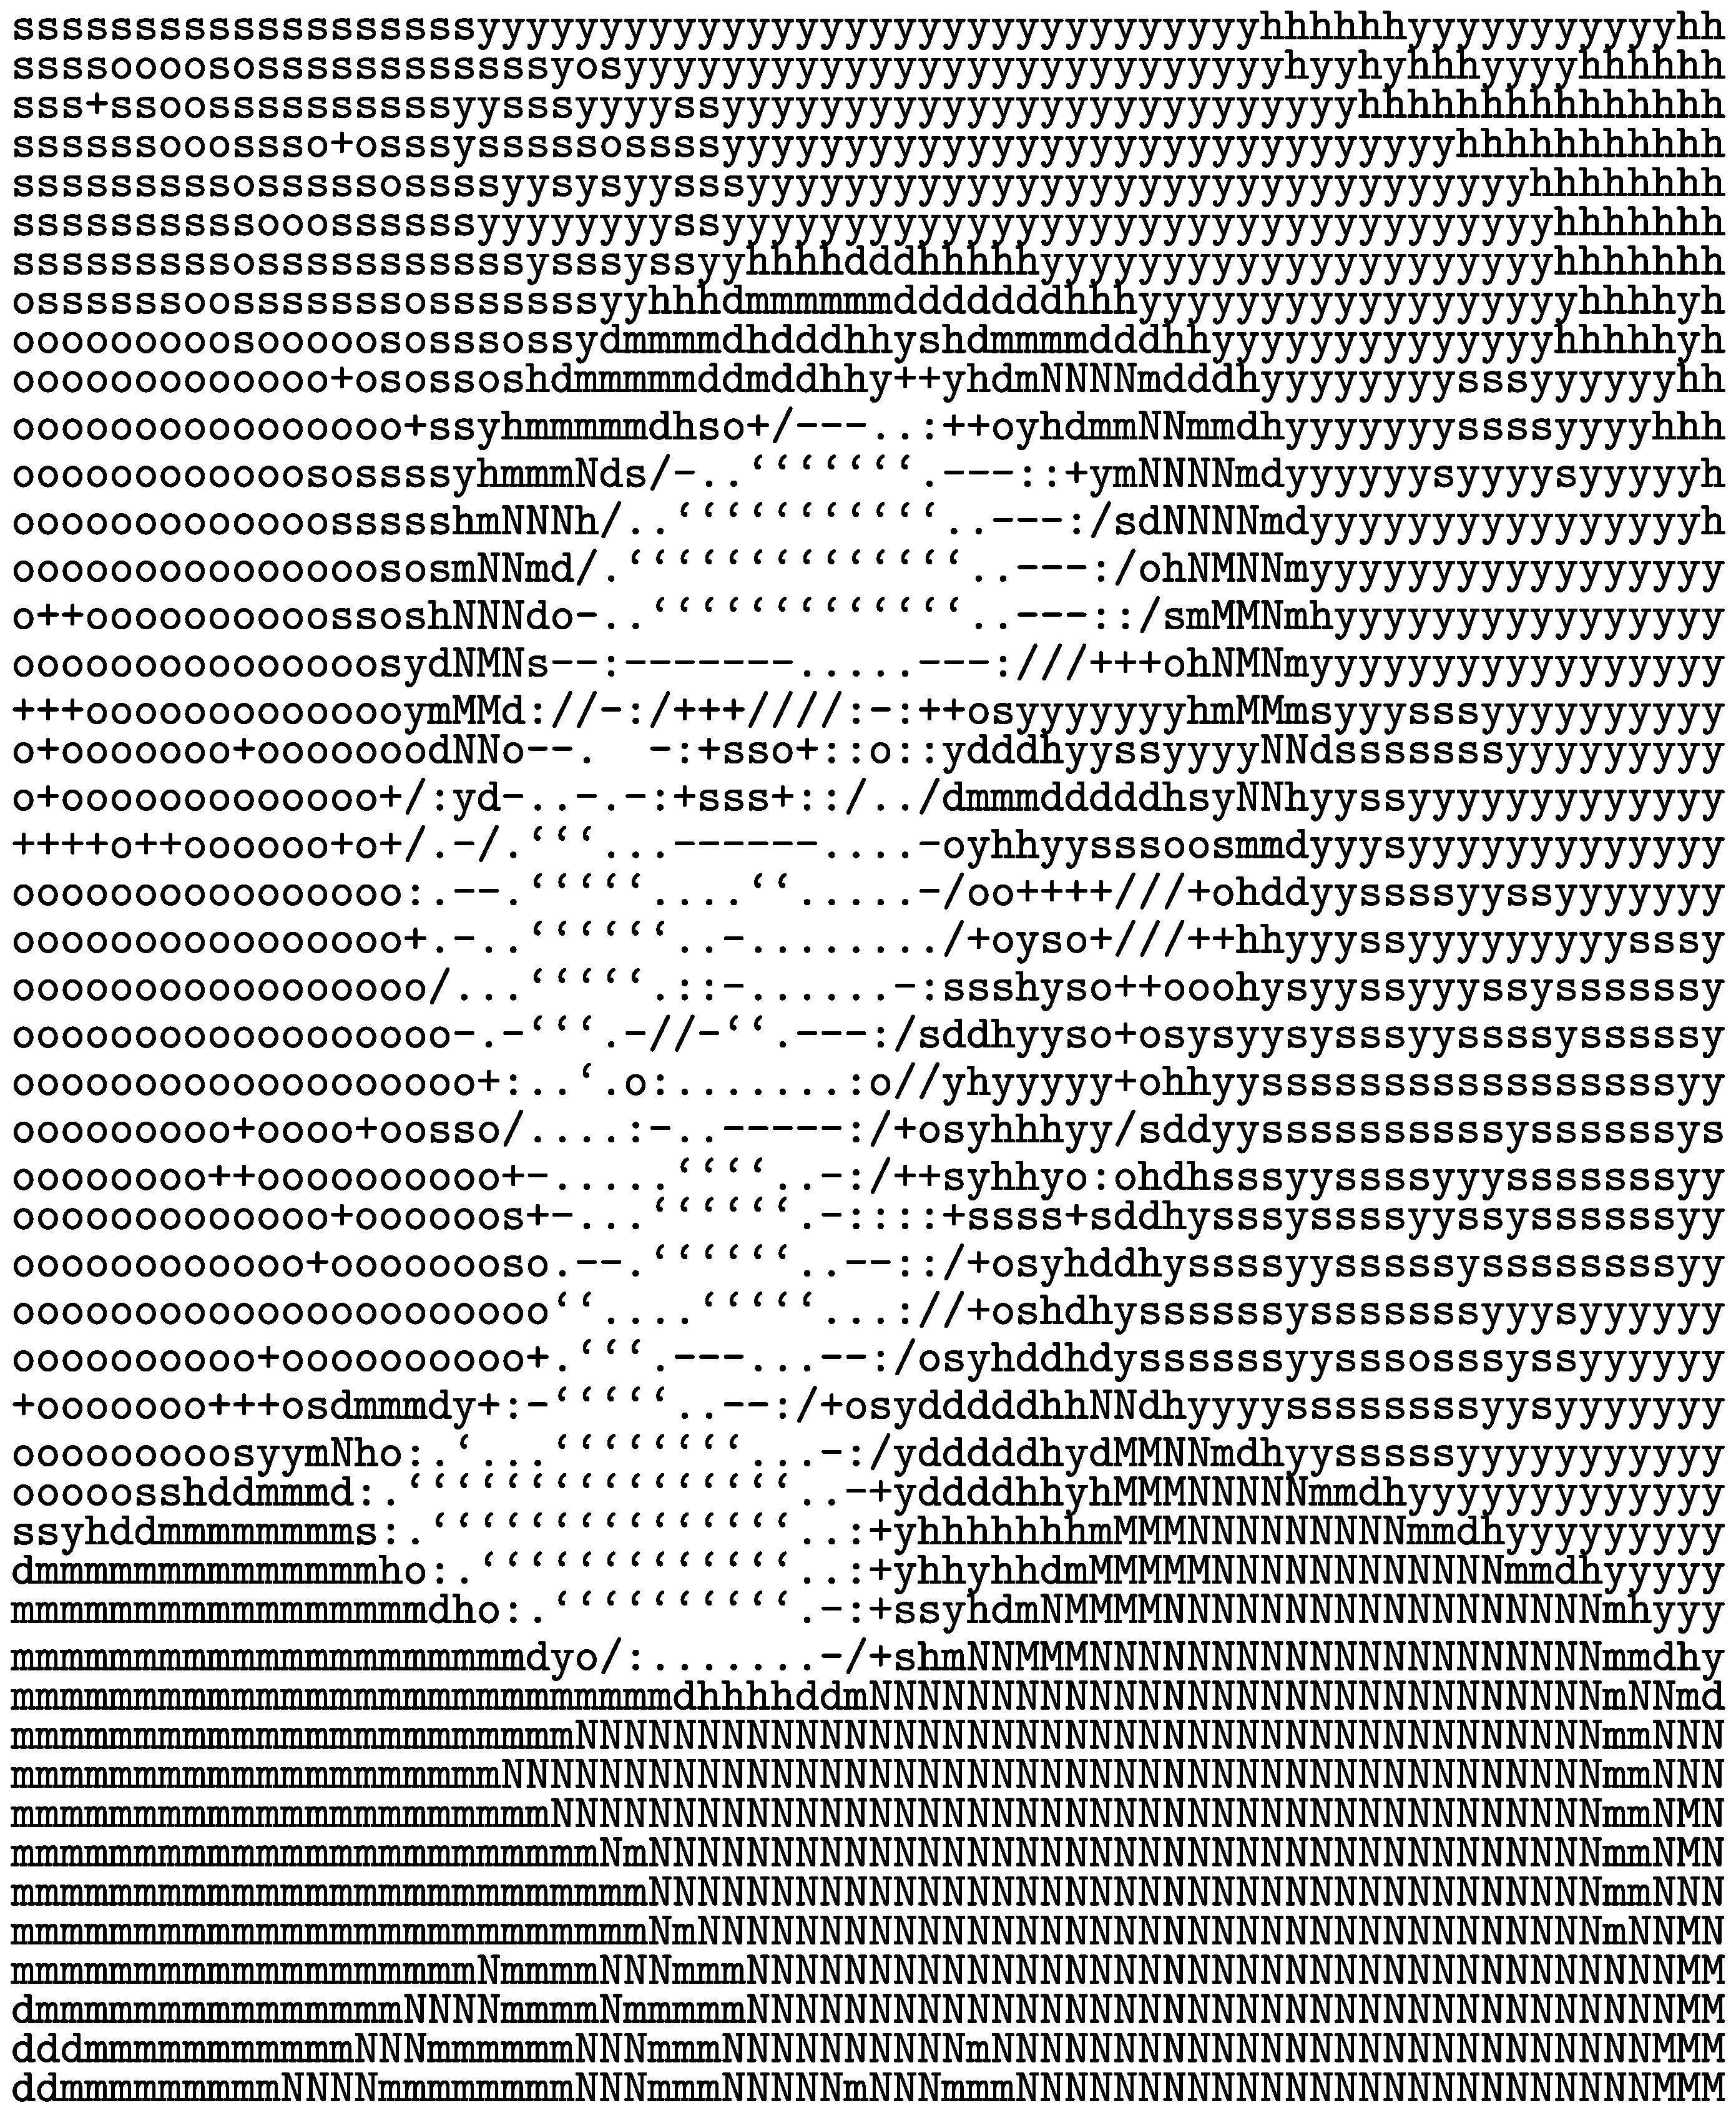
\includegraphics[width=\textwidth/2]{images/latex-image-1.eps}
\end{center}

\tableofcontents
%\include{index}
%\include{titlepg}
\mainmatter
\chapter{Introduction}

\begin{center}
\textbf{\begin{huge} October 25, 2011\end{huge}}
\end{center}

\section{Intro to cgs}

Mechanics:
\begin{center}
\begin{tabular}{c|c}
\hline
cgs &SI \\ \hline
cm & m\\ \hline
g & kg\\ \hline
s & s\\ \hline
erg & J\\ \hline
ergs/s & W\\ \hline
dyne & N \\
\hline
\end{tabular}
\end{center}

E\&M
\begin{center}
\begin{tabular}{c|c}
\hline
cgs &SI \\ \hline
k=1 & k=$\frac{1}{4\pi \epsilon_0}$ \\ \hline
$q_e = 4.8 \times 10^{-10}$ esu & $q_e = C$\\ \hline
$\mathbf{F} = q \frac{\mathbf{v}}{c} \times \mathbf{B} + q\mathbf{E}$ & $\mathbf{v}\times\mathbf{B}$\\  % WAIT WHAT
\hline
\end{tabular}
\end{center}

\section{Intro to Stars}

Sun:
\begin{list}{$^\circ$}{}
\item $L_\odot = 3.8 \times 10^{33} \textrm{ ergs s}^{-1} = 3.8 \times 10^{26}\textrm{ W}$
\item $R_\odot = 7 \times 10^{10} \textrm{ cm} \sim 10R_{\textrm{Jupiter}}$
\item $M_\odot = 2 \times 10^{33} \textrm{ g} \sim 10^3 M_{\textrm{Jupiter}} \sim 3\times 10^5 M_\oplus$
\item $t_\odot = 4.5 \times 10^9 \textrm{ years}$ 
\item $F_{BB} = \sigma T_{eff}^4$
\item $L = 4 \pi R_\odot^2 \sigma T_{eff}^4~, T_{eff} \approx 5800\textrm{ K}$
\item $T_c = 1.56 \times 10^7$ K, from neutrino measurements and sound waves
\end{list}

\begin{align}
< \rho_\odot> &= \frac{M}{\frac{4}{3}\pi R^3} \approx 1\textrm{ g cm}^{-3}\sim \rho_{\textrm{water}}\\
\rho_c &= 150 \textrm{ g cm}^{-3}\\
n &= \frac{\rho}{\mu m_p} \approx 10^{26} \textrm{ cm}^{-3}\\
&= n_e = n_p
\end{align}

Another way, $d$ = distance between particles; i.e., one particle per sphere of radius $d$. 
\begin{align}
n = \frac{4}{3}\pi d^3 = 1\\
d \approx \lp \frac{n}{\frac{4}{3}\pi }\rp^{-1/3} \sim n^{-1/3}
\end{align}
At the center of the sun, $d \approx 2 \times 10^{-9}$ cm, which is about the B\"ohr Radius ($a_0 \sim 10^{-8}$ cm).

An $e^-$ has 0 volume whereas if the size of a nucleus is $\sim 10^{-13}$ cm $ \ll$ distance between particles, then we can neglect inter-molecular forces and approximate the gas as an ideal gas. 

\section{Ideal Gas}

\begin{align}
P = n_e kT + n_p kT = 2n_p kT
\end{align}
At the center, $P \approx 2 \times 10^{17} \textrm{ ergs cm}^{-3}$. Photons have an intrinsic radiation pressure given by:
\begin{align}
P_{rad} &= \frac{1}{3}aT^4 \approx 10^{14}\textrm{ ergs cm}^{-3}~,a \textrm{ is the radiation constant}
\end{align}
If photons were degenerate, then instead:
\begin{align}
P = \frac{h^2}{5m_e} \lp \frac{3}{8\pi}^{2/3} \rp n_e^{5/3},
\end{align}
which stands true for an ideal QM gas of fermions, giving us $P_{\textrm{degen}} \approx 5 \times 10^{16} \textrm{ ergs cm}^{-3}$ at the center of the sun. $P_{\textrm{ideal}} \sim P_{\textrm{degen}}$, so our classical assumption of the state of gas in the sun isn't great. 

\subsection{Other Stars}

\begin{list}{$^\circ$}{}
\item$M \sim 0.1M_\odot - 100M_\odot$
\item $R \sim 0.1 - 1000R_\odot$
\item $L \sim 10^{-4} - 10^6 L_\odot$
\item $T_{eff} \sim \textrm{ few } 10^3 - 5 \times 10^4 \textrm{ K}$
\end{list}

On the Main Sequence, plotting $\ln \lp \frac{L}{L_\odot} \rp$ as a function of  $\ln \lp \frac{M}{M_\odot} \rp$, we see that $R \sim M^{0.75}, L \sim M^{3.5}, L\sim T^6$. For the most part, while on the MS, a star fuses H into He. Most stars spend most of their time in this phase. 

\chapter{Understanding the Basics of Stars}

\begin{center}
\textbf{\begin{huge} October 30, 2011\end{huge}}
\end{center}

\section{3 Key Pieces of Physics}

\begin{list}{$^\circ$}{}
\item Force Balance in stars: pressure \& gravity
\item Energy Transport: conduction, radiation, convection
\item Energy Generation: fusion and gravitational contraction
\end{list}

Each of these key pieces depends on the composition of the star which changes as a function of time. 

\section{Force Balance}
Let's look at a layer

\begin{figure}[!ht]
\centering
\includegraphics[width=\textwidth /2]{images/layers.ps}
\label{fig:layers}
\end{figure}

\begin{align}
M_{shell}&=Adr\rho\\
M_r& \equiv \textrm{ mass interior to point at $r$}
\end{align}
use $F=ma$
\begin{align}
M_{\textrm{shell}} a &= F_{\textrm{net}} = P_{\textrm{below}}A -P_{\textrm{above}}A - \frac{GM_rM_{\textrm{shell}}}{r^2}~,dr\ll r\\
P_{\textrm{above}} &= P_{\textrm{below}} + dP\\
M_{\textrm{shell}}a &= P_{\textrm{below}}A - (P_{\textrm{below}} + dP)A -\frac{GM_rM_{\textrm{shell}}}{r^2}\\
M_{\textrm{shell}}a &= \cancel{P_{\textrm{below}}A} - (\cancel{P_{\textrm{below}}} + dP)A -\frac{GM_rM_{\textrm{shell}}}{r^2}
\end{align}
want $M_{\textrm{shell}}a=0$ for Hydrostatic Equilibrium
\begin{align}
\cancel{A}dr\rho a &= -dP\cancel{A} - \frac{GM_r\cancel{A}dr\rho}{r^2}\\
\rho a &= -\frac{dP}{dr}-\rho\frac{GM_r}{r^2}
\end{align}
now assume $a=0 \ra $ no net force
\begin{align}
\boxed{\frac{dP}{dr} = -\rho\frac{GM_r}{r^2}}
\end{align}

assume $\rho\frac{GM_R}{r^2} > \frac{dP}{dr}$, drop pressure gradient so $a \sim -\frac{GM_r}{r^2}$. Let's say that $M_r \sim M, r\sim R$ so that $a \sim -\frac{GM}{R^2} \sim \frac{\Delta R}{t^2}$. What is the time such that gravity can move stuff a distance comparable to the size of the star? This is the ``Dynamical Timescale", or ``Freefall Timescale" of the star, represented as either $t_{dyn}$ or $t_{ff} \sim \sqrt{\frac{R^3}{GM}}$.

\subsection{Dynamical Timescale}
\begin{align}
\langle \rho \rangle &= \frac{3M}{4\pi R^3}\\
t_{dyn} &\sim \sqrt{\frac{R^3}{GM}} = \sqrt{\frac{1}{\langle \rho \rangle G}}~,\textrm{ sun:}\langle \rho \rangle = 1\textrm{ g cm}^{-3}\\
t_{dyn} &\sim 1\textrm{ hr}\ll 4.5 \times 10^9\textrm{ years}
\end{align}
This is why it's okay to assume that there is no imbalance of forces $\ra$ justification for Hydrostatic Equilibrium. 

\section{Scale Height}
But actually, imbalances within a star lead to sound waves. How are these detected?
\begin{align}
\Aboxed{M_r &= \int_0^r 4 \pi r^2 \rho dr}\\
\Aboxed{\frac{dM_r}{dr} &= 4\pi r^2\rho}
\end{align}

We can't solve $P = nkT$ because we have 2 equations ($M_r = ...~ \&~ \frac{dP}{dr} = ...$) and 3 unknowns ($P(\textrm{or }T),\rho,M_r$). To do this, let's look at the isothermal atmosphere (not the interior).\\

\begin{figure}[!ht]
\centering
\includegraphics[width=\textwidth /2]{images/isotherm_atmosphere.ps}
\label{fig:atmosphere}
\end{figure}

\begin{list}{$^\circ$}{}
\item $z=$ height above surface
\item $z=0$ at surface
\item assume $M_r$ = constant = $M$ (total mass)
\item assume $z \ll R$ so that $g$ is constant. 
\end{list}
We generally can't solve this unless you assume that $T = $ constant. If we do, then
\begin{align}
\frac{dP}{dz} &= kT \frac{dn}{dz} = -\rho g~,\rho = n\cdot \mu m_p\\
kT \frac{dn}{dz} &= -nmg\\
\int_{n(z=0)}^z \frac{dn}{n} &= \int_0^z -\frac{mg}{kT} = -\frac{mg}{kT}z\\
\ln \lp \frac{n(z)}{n(z=0)} \rp &= -\frac{mg}{kT}z\\
\Aboxed{n(z) &= n(z=0)e^{-z/h}~, h=\frac{kT}{mg}}
\end{align}
This is an ``exponential atmosphere" where $h$ is the scale height, the distance over which $n$ changes by approximately $\frac{1}{e}$. For comparison,
\begin{align}
\frac{h}{R} &= \frac{kT}{mgR}\\
&= \frac{kT}{\frac{GMm}{R}}\\
&= \frac{\textrm{KE or Thermal Energy}}{\textrm{Gravitational Potential Energy}}
\end{align}

If the thermal energy is larger, the atmosphere will be stretched higher up. For the sun,

\begin{align}
T_{eff}&= 5800\textrm{ K}\\
\frac{h}{r} &= 3 \times 10^{-4}~, h \approx 200\textrm{ km}
\end{align}
 
 Think of thus as a statistical mechanics problem with particles of temperature $T$ and energy $E$:
 \begin{align}
n(E) &\sim e^{-E/kT}
\end{align}

Above the surface a distance $z$, $g$ is pretty much constant and $n(z) = e^{-mgz/kT}$. 

\section{Mean Molecular Mass}

\begin{center}
\begin{tabular}{c|c}
\hline
neutral H & $m=m_p$ \\ \hline
ionized H & $m=\frac{1}{2}m_p$ \\ \hline
\end{tabular}
\end{center}

In other words, if you ionize the atmosphere, it will expand by a factor of 2.

Looking back at HE: 
\begin{center}
\begin{tabular}{c|c}
\hline
neutral H & $P=nkT$ \\ \hline
ionized H & $P =n_ekT + n_pkT = 2nkT$ \\ \hline
\end{tabular}
\end{center}

We see that ionized H has twice the pressure of neutral H.
\begin{align}
h &= \frac{kT}{mg}\\
&=\frac{2kT}{m_pg}
\end{align}

if $e^-$ and p don't have the same density profile, then
\begin{align}
e^- : h&= \frac{kT}{m_eg}\\
p: h&= \frac{kT}{m_pg}~,
\end{align}
but then the charge distribution is not neutral; we'd need an electric field to provide additional force. 

Let's assume a fully ionized gas of ions and electrons:
\begin{align}
P_{\textrm{ions}} = \sum_i n_ikT
\end{align}

Gravity only cares about the \textbf{total} mass density. To go from $n_i$ to $\rho$,
\begin{list}{$^\circ$}{}
\item $X_i$ = mass fraction of ion
\item $A_i$ = atomic \# (n \& p)
\item $n_i = \frac{X_i \rho}{m_pA_i}$
\end{list}

\begin{align}
P_{\textrm{ions}} &= \sum_i \frac{X_i \rho}{m_p A_i}kT\\
\Aboxed{&= \frac{\rho kT}{m_p} \sum_i \frac{X_i}{A_i} = \frac{\rho kT}{\mu_i m_p}}\\
\Aboxed{\frac{1}{\mu_i} &= \sum_i \frac{X_i}{A_i}~,\mu_i\textrm{ is the average mass per ion}}
\end{align}

For electrons, $P_e = n_ekT$.
\begin{align}
n_e &= \sum_i Z_in_i\textrm{ because the gas is fully ionized}\\
&= \sum_i \frac{X_iZ_i}{A_i}\frac{\rho}{m_p}\\
P_e &= \frac{\rho kT}{\mu_e m_p}~,\frac{1}{\mu_e} = \sum\frac{X_iZ_i}{A_i}
\end{align}
where $\mu_e$ is the electron mean molecular weight. 

\begin{align}
P_{\textrm{tot}} &= P_e + P_{\textrm{ions}} \\
&= \frac{\rho kT}{\mu_e m_p} +  \frac{\rho kT}{\mu_i m_p}\\
\Aboxed{&= \frac{\rho kT}{\mu m_p} ~,\frac{1}{\mu} = \frac{1}{\mu_e} + \frac{1}{\mu_i} = \sum_i \frac{X_i(1+Z_i)}{A_i}}
\end{align}

For ionized H, $Z_i = A_i = X_i = 1$, so $\mu = \frac{1}{2}$. Cosmic composition, by comparison, is 75\% H and 25\% He which turns out to be a $\mu$ of 0.62 or so.




\chapter{The Basics}

\begin{center}
\textbf{\begin{huge} September 4, 2011\end{huge}}
\end{center}

\section{Hydrostatic Equilibrium and the Virial Theorem}

\begin{align}
\int \frac{dP}{dr} &= -\rho g\\
&= -\int \frac{\rho GM_r}{r^2}\\
&= -\int \frac{\rho GM}{r^2}4 \pi r^3dr
\end{align}

Let's first solve each side individually and combine the results:

Right Hand Side:

\begin{align}
-\int_0^R \frac{GM_r}{r} 4 \pi r^2 \rho dr\\
\frac{dM_r}{dr}=4\pi r^2\rho\\
dM_r = 4 \pi r^2\rho dr\\
-\int_0^R \frac{GM_r}{r} dM_r \equiv U
\end{align}

Left Hand Side:

\begin{align}
&=\int_0^R \frac{dP}{dr}4\pi r^3 dr\\
\frac{d}{dr}(P 4 \pi r^3) = \frac{dP}{dr}4\pi r^3 + 3P4\pi r^2\\
&=\int_0^Rdr \lp \frac{d}{dr}\lp P4\pi r^3 \rp - 3P 4\pi r^2 \rp\\
&=\int_0^R \underbrace{dr \cdot  \frac{d}{dr}\lp P4\pi r^3 \rp}_{P 4 \pi r^3 \Bigl\lvert_0^R} - \underbrace{3 \int_0^R 4 \pi r^2drP }_{-3\int dVP}\\
&=P 4 \pi R^3 - P 4 \pi 0^3 - 3\int dVP~,\text{ but $P=0$ at surface, so $P4\pi R^3=0$}
\end{align}

\begin{align}
\langle P\rangle  &= \int_{P(r=0)}^{P(r=R)}dP\\
&= \frac{1}{V}dVP\\
&= \frac{3}{4 \pi R^3}\int dVP
\end{align}

Combining the LHS and RHS, 

\begin{align}
\Aboxed{-3\langle P\rangle V &= U}
\end{align}

This is the most general version of the Virial Theorem for stars. Now that we have this, let's derive relations between $P$ and $E$. First, what are the properties of stars?

\begin{list}{$\circ$}{}
\item $n=$ \# per unit time
\item $\overline{V}=$ velocity
\item $\overline{p} =$ momentum
\end{list}

Force on a wall $= \frac{\Delta p}{\Delta t}$. $PA = \frac{\Delta p}{\Delta t}$, $P = \frac{\Delta p}{\Delta t}\frac{1}{A}$.\\

\begin{align}
\frac{\Delta p}{\Delta t} = \# \text{ of collisions per unit time $\times~ \Delta p$ per collision}
\end{align}

For particles moving either way, 

\begin{align}
\frac{\Delta p}{\Delta t} &= n\cdot v_x \cdot A \cdot \half\\
\frac{\Delta p_x}{\Delta t} &= nv_xp_xA = PA\\
\frac{\Delta p_y}{\Delta t} &= nv_yp_yA = PA\\
\frac{\Delta p_z}{\Delta t} &= nv_zp_zA = PA\\
\frac{\Delta p}{\Delta t} &=\frac{1}{3}nA\overline{v}\overline{p} = PA\\
\frac{\Delta p}{\Delta t} &=\frac{1}{3}nvp = P\\
\Aboxed{P &= \frac{1}{3}n\langle pv\rangle}
\end{align}

\subsection{NR Virial Theorem}

For a NR gas of particles, $p=mv$

\begin{align}
P &= \frac{1}{3}n\langle mv^2\rangle\\
P &= \frac{2}{3}n\langle \half mv^2\rangle \\
P &= \frac{2}{3}n\langle K\rangle ~,\text{ KE is the energy per unit particle}\\
P &= \frac{2}{3}K~,\text{ per unit volume}
\end{align}

\begin{align}
U &= -3\langle P\rangle V\\
&= -3 \langle \frac{2}{3}K \rangle V\\
\Aboxed{U &= -2\langle K\rangle }\\
E_{TOT} &= U + K = \frac{U}{2}
\end{align}

What about a star where the kinetic energy is mostly dominated by relativistic particles?
\subsection{R Virial Theorem}

\begin{align}
P &= \frac{1}{3}n\langle pc\rangle \\
P &= \frac{1}{3}n\frac{K}{v}\\
U &= 3 \lp \frac{1}{3}nK \rp\\
\Aboxed{U &= -K}\\
E_{TOT} &= U + K = 0
\end{align}

If $E_{TOT} < 0$, the star is bound and stable. If $E_{TOT} = 0$, then the star is unstable. 

\section{Behavior of NR Stars}

For a NR star, $E_{TOT} = -K = \frac{U}{2}$. Let's say the star is losing heat to radiation and thus $E_{TOT}$ is decreasing. Because it's a gravitationally bound system, a loss in $E$ means that the star will contract and heat up. In other words, the star has negative heat capacity. \\

How long will it take for a star to go from $r=R$ to $r=\frac{R}{2}$? 

\begin{align}
\Delta U &\sim \frac{GM^2}{R}\\
&\sim \frac{GM^2}{ \lp\frac{R}{2} \rp}\\
&\sim \frac{2GM^2}{R}
\end{align}

Since we're dealing with Kelvin Helmholtz contraction, let's define a new time scale $t_{KH}$ defined to be $t_{KH} \approx \frac{E}{L}$. For our sun, $t_{KH} \approx 3 \times 10^7$ years $\ll 4.5 \times 10^9$ years, where the latter is the approximate current age of our sun. Therefore, KH contraction cannot explain fully the behavior of the sun; something else must be needed (fusion). 
\chapter{Energy Transport}

\begin{center}
\textbf{\begin{huge} September 6, 2011\end{huge}}
\end{center}

\section{Energy Transport by Conduction}
\begin{figure}[!ht]
\centering
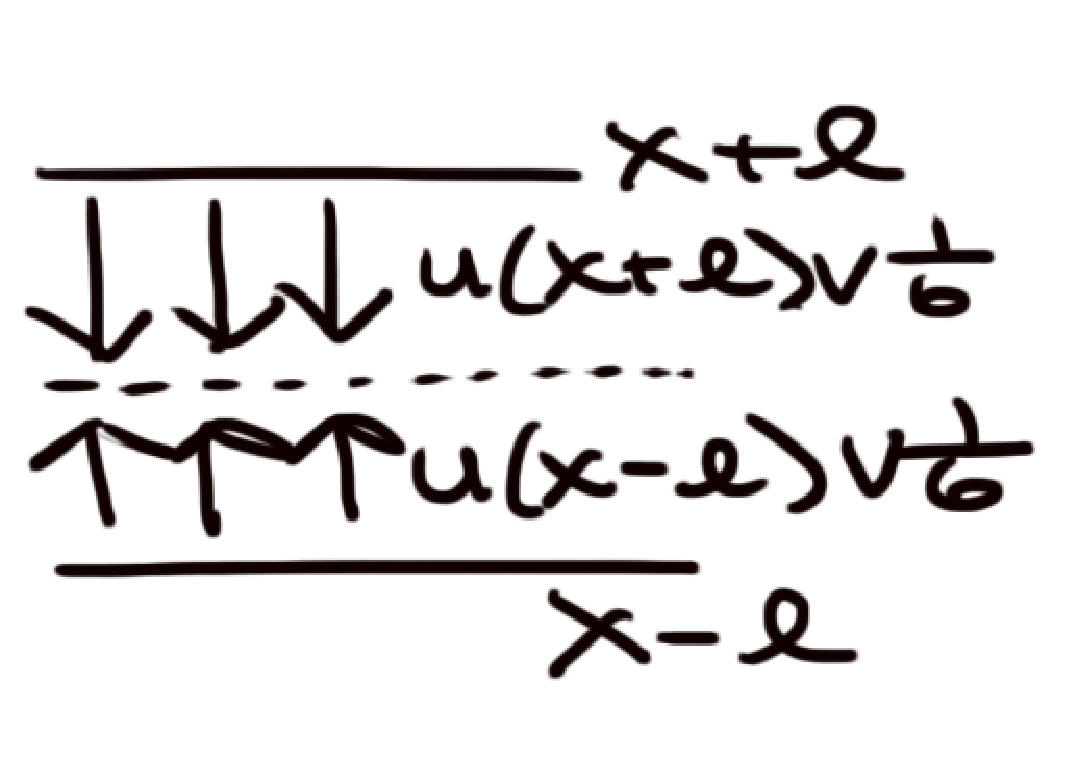
\includegraphics[width=\textwidth /2]{images/fig1.eps}
\label{fig:1}
\end{figure}

Figure \ref{fig:1} shows the stratification levels of the inside of a star at a given height $x$ with a length $l$  either up or down. \\
\begin{list}{}{}
\item $T$ = temp
\item $u$ = thermal Energy Density
\item $v$ = velocity
\item $l $= mean free path
\end{list}

The factor of $\frac{1}{6}$ is used because we multiply $\frac{1}{3}$ (from 3 degrees of translational freedom) with $\frac{1}{2}$ (from going up and down).

\begin{align}
F \equiv ~\text{net flux of energy} = \frac{1}{6}u(x-l)v - \frac{1}{6}u(x+l)v
\end{align}
Taylor expanding $u(x-l) = u(x) - \frac{du}{dx}l$, we get:

\begin{align}
F = -\frac{1}{3}vl\frac{du}{dx}~,~\text{or more generally,}~F=-\chi \nabla u
\end{align}

\subsection{Mean Free Path}
$\sigma$ is the collisional cross section of an individual particle. Flux can be defined as both $\frac{\text{\#}}{\text{area $\cdot$ time}}$ and $\frac{\text{\# of collisions}}{\text{sec}}$. The probability of colliding is $n \cdot dx \sigma$. The mean free path is the $dx$ where the probability of colliding is 1. $l = \frac{1}{n \sigma}$.\\
For neutral particles, $ R \sim a_0 \sim 0.5$\AA. $\sigma = \pi a_0^2 \sim 10^{-15}$ cm$^2$. In air, $l = \frac{1}{n \sigma}$ where $ n \sim 10^{20}$ cm$^{-3}$ which results in $l = 10^{-5}$ cm. \\

For a gas of charged particles,

\begin{align}
U &= n\frac{3}{2}kT\\
F &= -\frac{1}{3}vl \frac{dU}{dT}\frac{dT}{dx}~,~\text{where}~\frac{dU}{dT}~\text{is the specific heat}\\
\Aboxed{F &= -\frac{1}{2}nklv \frac{dT}{dx}}~.
\end{align}

In the case of a charged particle moving past another charged particle, there is a characterized distance $b$ where the change in trajectory is significant. 

\begin{align}
\frac{q^2}{b} &\sim kT\\
b &\sim \frac{q^2}{kT}\\
\text{effective area }=\sigma &= \pi b^2\\
\Aboxed{\sigma &= \frac{\pi q^4}{(kT)^2}}
\end{align}

\begin{align}
F &=-\frac{1}{2}nklv\frac{dT}{dx}~,v \sim v_{thm} = \sqrt{\frac{kT}{m}}\\
&\sim -\frac{1}{2} \frac{kv}{\sigma}\frac{dT}{dx}\\
&=-\chi \frac{dT}{dx}~,\text{where }\chi =\frac{1}{2}\frac{kv}{\sigma} \pt \frac{T^{5/2}}{\sqrt{m}}
\end{align}

Electrons move faster than protons so they transfer energy much more effectively. Electrons and protons have the same $\sigma$, but the difference in velocities is huge.

\subsection{How important is this energy transport in the sun?}

\begin{align}
F &= -\chi \frac{dT}{dx}\\
L &= 4 \pi R^2 F\\
&\sim 4 \pi R^2 \chi \frac{T_c}{R}~\text{(We're doing a poor man's derivative where $\frac{dT}{dx} = \frac{T_c}{R}$)}\\
L &\sim \frac{k^{7/2} T_c^{7/2} R}{q^4 \ln (\Lambda) \sqrt{m_e}}\\
&\sim 10^{-4} L_\odot \lp \frac{R}{R_\odot} \rp \lp \frac{T_c}{10^7\text{ K} } \rp^{7/2}
\end{align}

Doing this, we get that $L_{conduction} \ll L_\odot$ and therefore electron conduction is unimportant to energy transport. 

\section{Radiation Transport of Energy}
\begin{list}{}{}
\item $U = aT^4$
\item $l = \frac{1}{n \sigma} = \frac{1}{\kappa \sigma}$
\item $\sigma$ = cross section for photons to interact with matter, not with other photons
\end{list}

\begin{align}
F &=-\frac{1}{3}cl \frac{d}{dr}aT^4~,\chi = \frac{4}{3}claT^3 = \frac{4}{3}\frac{caT^3}{n\sigma} \\
&= -\frac{4}{3}claT^3 \frac{dT}{dr}\\
\Aboxed{&=-\frac{4}{3}\frac{caT^3}{\kappa \rho} \frac{dT}{dr}}
\end{align}

For an Ionized plasma with dominant photon-matter interactions through electron scattering (Thomson Scattering),

\begin{align}
m_e \overline{a} &= -e(\overline{E} + \frac{\overline{v}}{c} \times \overline{B})\\
|E| &= |B|\\
m_e\overline{a} &= -e\overline{E}\text{ since $ \frac{\overline{v}}{c} \times \overline{B}$ is small}\\
\overline{a} &= -\frac{e \overline{E}}{m_e}
\end{align}

\begin{align}
P &= \frac{2}{3}\frac{e^4}{c^3 m_e^2}|\overline{E}|^2\\
\sigma F &= P\\
\sigma \frac{c}{4\pi}|\overline{E}| &= \frac{2}{3}\frac{e^4}{c^3 m_e^2}|\overline{E}|^2\\
\Aboxed{\sigma_T &= \frac{8\pi}{3}\frac{e^4}{m_e^2 c^4} = \text{ Thomson cross-section or $e^-$-scattering cross-section}}
\end{align}

\begin{align}
\sigma_T &= \frac{8\pi}{3}r_c^2,~\text{ where $r_c$ is the classical radius of the $e^-$}\\
r_c &=\frac{e^2}{m_e c^2} \approx 2.8 \times 10^{-13} \text{ cm},
\end{align}
which should strike as odd since $e^-$ has no observed structure but still has an ``effective radius".
\chapter{Conduction}

\begin{center}
\textbf{\begin{huge} September 8, 2011\end{huge}}
\end{center}

\section{Picking Up Where We Left Off}
\begin{align}
F &= -\frac{4}{3}\frac{caT^3}{\kappa \rho} \frac{dT}{dr} \leftarrow \text{ for radiative diffusion}\\
&= -\frac{1}{3}lc \frac{dU}{dr}
\end{align}

Applying it:

\begin{align}
\frac{dT}{dr} \sim -\frac{T}{R}\\
L \sim \chi M^3~, kT \sim \frac{GM \mu m_p}{R}\\
\chi = \frac{a (\mu m_p)^4 cG^4 \mu_e m_p}{\sigma_T \kappa^4}\\
L \sim 10^{35} \lp \frac{M}{M_\odot} \rp ^3 \text{ ergs/s}\\
L \sim L_\odot~,e^- \text{ conduction $L \ll L_\odot$ so photons are dominating}
\end{align}

$L$ is strictly \textit{NOT} dependent on fusion, it is more dependent on $\frac{dU}{dT}$ of the photons. Fusion creates $E$ and the photons but doesn't determine the rate of energy leaving.\\
$\chi$ is constant, but dependent on the composition of the star. 

\begin{align}
L \pt \mu^4 \mu_e M^3\\
H \rightarrow HE\\
\mu \rightarrow \mu \uparrow\\
L \rightarrow L \uparrow
\end{align}

$L$ was lower in the past. $L$ when the Earth forced was only 20\% of the current $L_\odot$. This brings about the problem that the Earth was supposedly a ball of ice during it's evolution. \\

\begin{align}
\frac{3}{2}nkT > aT^4\\
F &= -\frac{1}{3}lv \frac{dU}{dx}\\
&= -\chi \frac{dT}{dx},\chi = \frac{1}{3}lv \frac{dU}{dT}\\
\frac{F_{rad}}{F_{e^-}} &= \frac{-\chi_{rad}}{-\chi_{e^-}}, \frac{dT}{dx}\text{ is the same for both}\\
&\sim \frac{l_\gamma}{l_{e^-} }\frac{ c}{v_{e^-} }\frac{aT^4}{\frac{3}{2}nkT}
\end{align}

$ \frac{l_\gamma}{l_{e^-} } \ggg 1$, $\frac{ c}{v_{e^-}} \gg 1$, and $\frac{aT^4}{\frac{3}{2}nkT} \ll 1$.\\

\begin{align}
F = -\frac{4}{3}\frac{caT^4}{n \sigma} \frac{dT}{dr}
\end{align}

We want to find the time for thermal energy to leak out by photon diffusion.

\begin{align}
t_{KH} &= \frac{E}{L}\\
L &\sim 4 \pi R^2 \frac{4}{3}aT^3 \frac{1}{n\sigma}\frac{T}{R}\\
&= \frac{\frac{3}{2}nkT \cdot \dfrac{4}{3}\pi R^3}{ \lp \dfrac{4 \cdot 16 \pi aT^4R}{R3n\sigma} \rp}\\
&=\frac{\frac{3}{2}nkTR^2n\sigma}{4aT^4c}\\
&\sim \frac{nkT}{aT^4}\frac{R^2}{lc}\\
&\sim \frac{nkT}{aT^4}t_{RW}~,\text{ where $t_{RW}=\frac{R^2}{lc}=$ random walk time}
\end{align}

\begin{align}
<|D|^2>&=Nl^2~,\text{ where $N = $ number of steps}\\
<|D|^2>^{1/2} &= \text{ RMS Distance = typical distance a photon will find itself after $N$ scatterings}\\
&= \sqrt{N}l
\end{align}

What is $N$ so that the photon leaves the star?

\begin{align}
<|D|^2>^{1/2} &=R\\
N &\sim \lp \frac{R}{l} \rp^2\\
\frac{R}{l} \sim 10^{11},N\sim 10^{22}
\end{align}

How long does it take to get out? 

\begin{align}
Nt_{step} = t_{esc} = N\frac{l}{c} \sim \lp \frac{R}{l} \rp^2 \cdot \frac{l}{c} \sim \frac{R^2}{lc}\\
\sim 10^4 \text{ years for our sun}
\end{align}

If photons didn't bounce around, it would escape in 2 seconds. ($\nu_e$ can get out in about 2 seconds, $l_\nu$ must be greater than $R_\odot$) Also, the time it takes for heat to diffuse throughout a room is: $\frac{R^2}{lv_{thm}}$.

\begin{align}
F &= -\frac{4}{3}\frac{caT^4}{n \sigma} \frac{dT}{dr}\\
&= -lc \frac{d}{dr}\frac{1}{3}aT^4\\
F_r &= -lc\frac{d}{dr}P_{rad}~,\text{ we must be careful, $F$ and $L$ depend on $r$}\\
\frac{L_r}{4\pi r^2} &= -lc \frac{d}{dr}P_{rad}\\
-\frac{L_r}{4\pi lc r^2} &= \frac{d}{dr}P_{rad}\\
-\frac{L_r \kappa \rho}{4\pi c r^2} &= \frac{d}{dr}P_{rad}\\
\end{align}

We're interested in how $P_{rad}$ changes with $P_{tot}$. 

\begin{align}
\frac{dP_{rad}}{dP} = \frac{L_r \kappa}{4 \pi G M_r c} \equiv \frac{L_r}{L_{EDD}}
\end{align}

Roughly, if $P_{rad} \sim P_{tot}$, then $L_r \sim L_{EDD}$.

\subsection{Eddington Luminosity}

\begin{list}{}{}
\item $F_g = -\frac{GMm}{r^2}$
\item $F_{rad} = \frac{dp}{dt}$
\item $p_{proton} = \frac{E}{c} = \frac{h \nu}{c} = \frac{h}{\lambda}$
\end{list}

What is the total $p$ per unit time produced by the star? $\sum\limits{_i^\infty} p_i $ is too hard...

\begin{align}
p_{photon} = \frac{E}{c} = \frac{L}{c}\\
F_{Rad} = \frac{dp}{dt} = \frac{L}{c 4\pi r^2} \sigma
\end{align}

The Eddington Luminosity is where the radiation force equals the forge of gravity. The Eddington "Limit" is:

\begin{align}
L_{EDD} = \frac{4 \pi G Mc}{\sigma /m} = \frac{4 \pi G Mc}{\kappa}
\end{align}

If $L > L_{EDD}$, $F_{rad} > F_{grav}$, and material is "blown" out. 

\subsection{Fully Ionized H}

\begin{list}{$\circ$}{}
\item $L_{EDD} = \frac{4 \pi GMc}{\kappa}$
\item $\kappa = \frac{\sigma_T}{m}$
\item $l = \frac{1}{n \sigma} = \frac{1}{n_e \sigma_T} = \frac{1}{\kappa \sigma}$
\item For fully ionized $H$, $\mu_e =1$
\item since photons are only interacting with $e^-$ and not $p$, $\mu = 1 = \mu_e$
\end{list}

\begin{align}
\kappa &= \frac{\sigma_T}{m}\\
&= 0.4\text{ cm}^2\text{ g}^{-1}
\end{align}

\begin{align}
L_{EDD} = 1.3 \times 10^{38} \lp \frac{M}{M_\odot} \rp \text{ ergs s}^{-1}
\end{align}

\begin{list}{}{}
\item If $L \sim L_{EDD}$, $F_{rad} \sim F_{grav}$ which results in the radiation force not being important in the sun. It's dominated by gas pressure.
\item As $M \uparrow, L_{EDD} \uparrow$ so higher $M$ means $P_{rad}$ becomes more important $\rightarrow$ it becomes the dominant force
\end{list}


\chapter{Convection}

\begin{center}
\textbf{\begin{huge} September 13, 2011\end{huge}}
\end{center}

\section{Convection}
Second Law of Thermodynamics: $TdS = dE + PdV$, which isn't all that useful for stars, really.
\begin{list}{}{}
\item $U = \frac{E}{\mu}$: Energy per unit mass
\item $s = \frac{S}{U}$: Entropy per unit mass
\item $M =$ conserved, $l$ is small
\item $\rho = \frac{M}{V}, V = \frac{M}{\rho} \rightarrow \boxed{dV = -d\rho \frac{M}{\rho^2}}$
\item $\frac{TdS = dE + PdV}{\mu} = \boxed{ TdS = dU - \frac{P}{\rho^2}d\rho }$  : second law, for astrophysicists
\end{list}

\subsection{Review of the Adiabatic Process}

\begin{align}
\epsilon = E/\text{unit volume},\text{ NR}: P &= \frac{2}{3} \epsilon\\
\text{R}: P &= \frac{1}{3} \epsilon\\
U = \frac{\epsilon}{\rho} = \frac{P}{\rho} = \phi U~,\text{ where $\phi$ is either $1/3$ or $2/3$}\\
dU = \frac{P}{\rho^2}d\rho = \phi U\frac{d\rho}{\rho}\\
\frac{dU}{U} = \phi \frac{d\rho}{\rho}\\
U \pt \rho^\phi~,\text{ for an adiabatic process}\\
P \pt \rho U \pt \rho ^{\phi+1} \pt \rho^{\gamma}~,  \phi + 1  = \gamma =\text{ the adiabatic index}\\
\end{align}

\begin{align}
\text{For a NR gas: } \phi = \frac{2}{3}, \gamma = \frac{5}{3}~,P\pt \rho^{5/3}, T \pt \rho^{2/3}\text{ for an adiabatic process}\\
\text{For a R gas: } \phi = \frac{1}{3}, \gamma = \frac{4}{3}~,P\pt \rho^{4/3}, T \pt \rho^{1/3}\text{ for an adiabatic process}
\end{align}

\subsection{What is the Entropy of an Ideal Gas?}

\begin{align}
TdS &= dU - \frac{P}{\rho^2}d\rho\\
\frac{TdS}{U} &= \frac{dU}{U} - (\gamma - 1)\frac{U\frac{d\rho}{\rho}}{U}\\
U &=\frac{P}{\rho}\frac{1}{\gamma -1} = \frac{1}{\gamma - 1} \frac{kT}{m}\\
\frac{m(\gamma -1)}{k}dS &= \frac{dU}{U} - (\gamma -1)\frac{d\rho}{\rho}\\
\frac{m(\gamma - 1)}{k}s &= \ln U - (\gamma - 1)\ln \rho + c\\
\Aboxed{s &= \frac{k}{m}\frac{1}{\gamma - 1} \ln \lp \frac{U}{\rho^{\gamma - 1}} \rp  +c}\\	
s &= \frac{k}{m} \frac{1}{\gamma -1} \ln \lp \frac{P}{\rho^\gamma} \rp + c
\end{align}

For an adiabatic process, $s=0 \rightarrow \frac{k}{m} \frac{1}{\gamma -1} \underbrace{\ln \lp \frac{P}{\rho^\gamma} \rp}_{P \pt \rho^\gamma} + c$

\begin{align}
\frac{Tds}{dt} &= \underbrace{\frac{dU}{dt}}_{\text{heating}} - \underbrace{\frac{P}{\rho^2}\frac{d\rho}{dt}}_{\text{cooling}}\\
&= \underbrace{E_{heat}}_{\text{fusion}} - \underbrace{\frac{1}{\rho}(\overline{\nabla} \cdot \overline{F})}_{\text{photon convection}}
\end{align}

Say a blob is gaining/losing heat. $E_{fusion}$ is the heating per mass per time and $\overline{F}$ is the flux of $E$. In general:

\begin{align}
\text{total cooling} &= \int \overline{F}\cdot d\overline{A}\\
&= \int \overline{\nabla} \cdot \overline{F} d\overline{V}\\
\text{cooling per unit $V$} &= \overline{\nabla} \cdot \overline{F}\\
\text{cooling per unit mass} &= \frac{1}{\rho}(\overline{\nabla} \cdot F)
\end{align}

If a blob moves up a distance $dr$, given $T(r), P(r),$ and $\rho(r)$, is the fluid buoyantly stable? i.e. $\rho_{blob} \gtrless \rho_\star$? We'll be making 2 assumptions which we will then confirm \textit{post-facto}. 
\begin{list}{$\circ$}{}
\item Motion is adiabatic $\leftarrow$ valid if the time scale to move ($\sim$ 1 month) is sufficiently smaller than the time to exchange heat with the surroundings ($\sim10^7$ years)
\item $P_{blob} = P_\star$ at all times; in pressure equilibrium with surroundings
\end{list}

The time scale to establish HE: $\sim\frac{1}{\sqrt{G\rho}} \sim 1 $ hr $\ll$ time to move $dr$, which is about a month. If it's adiabatic, $s_{blob} = s \ne s_\star$ in general, where $s_{blob}$ is the blob at the new position, $s$ is the initial entropy, and $s_\star$ is the background entropy of the star at the new position.\\

\begin{center}
\begin{tabular}{c|c}
\hline
$\dfrac{ds}{dr} < 0$ & $\dfrac{ds}{dr} > 0$\\ \hline
$s>s_\star$ & $s < s_\star$\\ \hline
$s_{blob} > s_\star$ & $s_{blob}< s_\star$\\ \hline
$P_{blob} = P_\star$ & $P_{blob} = P_\star$\\ \hline
$\rho_{blob} < \rho_\star$ & $\rho_{blob} > \rho_\star$ \\ \hline
buoyancy unstable, rises & sinks back down (stable)\\
\hline
\end{tabular}
\end{center}


\chapter{More Convection}

\begin{center}
\textbf{\begin{huge} September 15, 2011\end{huge}}
\end{center}

\section{Models}
Blob's motion is adiabatic: $s_{blob} = s \ne s_\star$. The blob is in pressure and pressure equilibrium with it's surroundings. The time scale for the blob to move is $\ll t_{{\text dynamic}}$ or $t_{{\text sound~crossing}}$. 

\begin{align}
s \pt \ln \lp \frac{P}{\rho^\gamma} \rp : \frac{ds}{dr}<0~, s_{blob} = s > s_\star~,\rho_{blob} < \rho_\star
\end{align}

At the new position, $a = g \frac{\Delta \rho}{ \rho} = |\overline{g} | \lp \frac{\rho_\star - \rho_{blob}}{\rho_{blob}} \rp$. If $\rho_{blob} > \rho_\star$, $a$ is negative and it goes back down. If $\rho_{blob} < \rho_\star$, then $a$ is positive.

\subsection{Background Stellar Model}

\begin{align}
\boxed{\rho_\star = \rho + \frac{d \rho}{dr} \delta r}~,\text{ where $ \frac{d \rho}{dr}$ is the $\rho$ gradient of the stellar model}
\end{align}

This, however, is quite boring. 

\begin{align}
P_\star &= \rho + \frac{d\rho}{dr}\delta r\\
&= P_{blob} = P  + \delta P\\
\delta P &= \frac{dP}{dr}\delta r
\end{align}

\subsection{Blob Model}

\begin{align}
\rho_{blob} &= \rho + \underbrace{\lp \frac{\delta \rho}{\delta P} \rp_s}_{\text{adiabatic}} \delta P~, \text{ able to calculate $\delta P$ from $P_{\text{blob}} = P_\star$}\\
P &\pt \rho^\gamma\\
\lp \frac{\delta P}{\delta \rho} \rp_s &= \gamma \frac{P}{\rho}\\
\lp \frac{\delta \rho}{\delta P}\rp_s = \frac{\rho}{\gamma P}\\
\rho_{blob} &= \rho + \frac{\rho}{\gamma}\frac{\delta P}{P}\\
\Aboxed{\rho_{blob} &= \rho + \frac{\rho}{\gamma} \frac{d \ln P}{dr} \delta r}
\end{align}

\begin{align}
a &= g  \lp \frac{\rho_\star - \rho_{blob}}{\rho_{blob}} \rp\\
&= g \lp \frac{\rho + \frac{d\rho}{dr} \delta r}{\rho + \frac{\rho}{\gamma} \frac{d \ln P}{dr}\delta r} - 1 \rp~,\text{ assuming that $\delta r$ is really small}
\end{align}

\begin{align}
a &\equiv -N^2\delta r\\
N &= -g \lp \frac{d \ln \rho}{dr} - \frac{1}{\gamma} \frac{d \ln P}{dr} \rp\\
&= \frac{\gamma -1}{\gamma} \frac{m}{k}g \frac{ds}{dr}
\end{align}

$[N] = \frac{1}{s}$, the Brunt-V\"ais\"al\"a Frequency. Whether or not convection sets in or not is only dependent on $\frac{ds}{dr}$. 

\begin{align}
a = \frac{d^2}{dt^2}\delta r = -N^2 \delta r\\
\boxed{\frac{d^2}{dt^2}\delta r + N^2 \delta r = 0}~,\text{ Equation of Motion}
\end{align}

If $N^2 > 0$, then $\delta r \pt e^{iNt} \pt  \cos(Nt)  + i\sin(Nt)$. This is a stable oscillatory solution. If you push it a little bit, it'll oscillate. If $N^2 < 0, \frac{ds}{dr} < 0, \delta r \pt e^{|N|t}$, which is an exponentially growing solution on a time scale $\frac{1}{N}$ and is dubbed "convection". Say for example we know $dP, d\rho, ds$, then we know if it's spontaneously boiling.\\

\subsection{Will Convection Set In?}

Convection sets in if:

\begin{align}
\frac{ds}{dr} < 0\\
N^2 < 0\\
s &\pt \ln \lp \frac{P}{\rho^\gamma} \rp\\
 &\pt \ln \lp \frac{T^\gamma}{P^{\gamma -1}} \rp\\
P = \frac{\rho kT}{\mu m_p}\\
\rho \pt \frac{P}{T}~.
\end{align}

\begin{align}
\gamma \frac{d \ln T}{dr} &< ( \gamma - 1) \frac{d \ln P}{dr}\\
\underbrace{\frac{d \ln T}{dr}}_{\text{$-$ sign}} &< \frac{\gamma -1}{\gamma}\underbrace{\frac{d \ln P}{dr}}_{\text{$-$ sign}}\\
\Aboxed{\Bigl\lvert \frac{d \ln T}{dr} \Bigl\lvert &> \frac{\gamma -1}{\gamma} \Bigl\lvert \frac{d \ln P}{dr} \Bigl\lvert} \\
\text{or}\\
\Bigl\lvert \frac{d \ln T}{d \ln P	} \Bigl\lvert &> \frac{\gamma - 1}{\gamma} = \frac{2}{5}~,\gamma = \frac{5}{3}
\end{align}

We can calculate $\frac{dT}{dr}$ if the photons carry the energy.

\begin{align}
\Bigl\lvert \frac{d \ln T}{dr} \Bigl\lvert &> \frac{\gamma -1}{\gamma} \Bigl\lvert \frac{d \ln P}{dr} \Bigl\lvert\\
\text{Combine HE \& RD: } \frac{dP_{rad}}{dP} &= \frac{L_r \kappa}{4 \pi GM_r c}\\
\frac{P}{P_{rad}}\frac{dP_{rad}}{dP} &= \frac{L_r \kappa}{4 \pi GM_r c}\frac{P}{P_{rad}}~,\frac{P}{dP} = \frac{1}{d \ln P}\\
\Aboxed{\frac{d \ln P_{rad}}{d \ln P} &=4 \frac{d \ln T}{d \ln P}}
\end{align}

Quick note about the $d \ln T$ stuff: take for example $P\pt T_{rad}^4$. $\ln P_{rad} \pt 4 \ln T +$ constant. $\frac{d}{d \ln T} \ln P_{rad} = \frac{d}{d \ln T}4 \ln T +$ constant$= 4$.\\
If photons carry the energy, can directly calculate: 

\begin{align}
\boxed{\frac{d \ln T}{d \ln P} = \frac{1}{4} \frac{P}{P_{rad}} \frac{L_r \kappa}{4 \pi GM_rc}}
\end{align}

Another way to think about it is that if 

\begin{align}
\frac{d \ln T}{d \ln P} > \frac{\gamma -1}{\gamma}~,
\end{align}

then convection sets in.

\section{Our $\odot$}

For our sun, convection occurs in a radius about $r \gtrsim 0.7 R_\odot$. At the enter of the sun, $T\sim 10^7$ K. At larger $r$, $T \downarrow$ and $\kappa \uparrow$. 

\begin{align}
\frac{d \ln T}{d \ln P} > \frac{2}{5}~,\text{ at higher $r$, convection is determined by $\kappa$}
\end{align}

In the region between $0 < r \lesssim 0.7R_\odot$, the sun is relatively much hotter than its other parts and thus photons can carry the energy out. The $l$ per photons is relatively large and streaming out isn't a problem. As you extend outwards, however, $T \downarrow, \kappa \uparrow$, resulting in a higher $N$ (where in this case $N$ is the number of RW steps). Photons now have trouble moving the energy and convection takes over. \\

$M < M_\odot, T < T_\odot, \kappa \uparrow$, and more convection. For stars with $M \lesssim \frac{1}{3}M_\odot$, they are fully convective. $M > M_\odot, T > T_\odot, \kappa \downarrow$, the surface convection zone goes away, BUT the core now becomes convective. What actually happens when convection moves energy?

\section{Energy Transport by Convection}

Let's say there are two blobs, one with a high $\rho$ and low $T$ and another with a low $\rho$ and a high $T$. The blobs with high $\rho$ will sink and the blob with low $\rho$ will rise. This makes sense, hot stuff rises, cold stuff sinks. 

\begin{align}
v_c = \text{ typical convective velocity}\\
F_c &\sim \frac{1}{2}\rho v_c^2 \cdot v_c \\
\Aboxed{&\sim \frac{1}{2} \rho v_c^3}\\
\text{OR}\\
\Aboxed{F_c &\sim \rho \Delta E \cdot v_c}
\end{align}

Since $d\rho$ is so small, able to use either. Let's determine the $v_c$ through the work done by buoyancy. When a blob rises from one position to another, it moves from a region of high $P$ to a region of lower $P$. The blob shares energy with it's surroundings and must enlarge to conserve mass. 

\begin{align}
l \equiv \alpha H~,\text{ H is the scale height},H = \lp \frac{d \ln P}{dr} \rp^{-1}
\end{align}

How much energy goes the blob gain?

\begin{align}
a \equiv |N|^2\delta r\\
E_{gained/mass} = \frac{1}{2}\rho v_c^2\\
v_c^2 &= |N|^2 \delta r\\
v_c^2 &= |N|^2l^2\\
&= \alpha^2 H^2 |N|^2~,|N|^2 = g\frac{1}{c_p} \frac{ds}{dr}
\end{align}


\chapter{Finishing Convection}

\begin{center}
\textbf{\begin{huge} September 20, 2011\end{huge}}
\end{center}

\section{Convection Continued}

\begin{align}
a = |N|^2 \delta r\\
|N|^2 &= \frac{g}{c_p} \Bigl\lvert \frac{ds}{dr} \Bigl\lvert\\
&= \frac{g}{H} \Bigl\lvert \frac{H}{c_p} \frac{ds}{dr} \Bigl\lvert\\
v_c^2 = a \delta r = |N|^2 \delta r^2\\
\delta r \equiv \alpha H\\
v_c = \alpha c_s \Bigl\lvert \frac{H}{c_p} \frac{ds}{dr} \Bigl\lvert^{1/2}\\
F = \frac{1}{2}\rho v_c^3 = \frac{1}{2} \rho \alpha ^3 c_s^3 \Bigl\lvert \frac{H}{c_p} \frac{ds}{dr} \Bigl\lvert ^{3/2}\\
c_s^2 = \frac{kT}{\mu m_p} = \frac{P}{\rho}
\end{align}

We wanted to find the $F_r = -\frac{4}{3} \frac{caT^3}{\kappa \rho}\frac{dT}{dr}$ equivalent for convection. $F = \frac{1}{2}\rho v_c^3 = \frac{1}{2} \rho \alpha ^3 c_s^3 \Bigl\lvert \frac{H}{c_p} \frac{ds}{dr} \Bigl\lvert ^{3/2}$ gives the $v_c$ and $\frac{ds}{dr}$ given the flux. \\

$\Bigl\lvert \frac{H}{c_p} \frac{ds}{dr} \Bigl\lvert \sim 10^{-6}$, $s \sim c_p$, so $\frac{\Delta s }{s} \sim 10^{-6}$ on a length scale $\sim H$. Ergo, $s$ = constant in the convection zone. This replaces $F_r = -\frac{4}{3} \frac{caT^3}{\kappa \rho}\frac{dT}{dr}$. Let's assume $P \pt \rho^\gamma$ \& $\frac{dP}{dr} = -\rho \frac{GM_r}{r^2}$. 

\begin{align}
\frac{dM_r}{dr} = 4 \pi r^2 \rho\\
\frac{d}{dr} \lp \frac{r^2}{\rho} \frac{dP}{dr} = -\rho GM_r \rp\\
\frac{d}{dr} \lp \frac{r^2}{\rho	} \frac{dP}{dr} \rp = -4\pi r^2 G\rho
\end{align}

But... if $P = K \rho^\gamma$, $\frac{dP}{dr} = \gamma K \rho^{\gamma-1} \frac{d\rho}{dr}$! These kinds of models are called:

\subsection{Polytropic Models}

\begin{align}
P &= K\rho^\gamma\\
&= K \rho^{1 + 1/n}, \gamma = 1 + \frac{1}{n}, \text{ where n is the polytropic index}
\end{align}

\begin{align}
\theta = \lp \frac{\rho}{\rho_c} \rp ^{1/n}~,\rho_c = \rho(r=0)\\
\zeta = \frac{r}{a}~, a = \sqrt{\frac{(n+1) K \rho_c ^{\frac{1}{n} -1}}{4 \pi G}}~,[a] = \text{ cm}
\end{align}

\begin{align}
\underbrace{\boxed{\frac{1}{\zeta^2} \cdot \frac{d}{d\zeta} \lp  \zeta^2 \frac{d\theta}{d\zeta} \rp = -\theta^n}}_{\text{Lane-Emden Equation}}
\end{align}

Boundary conditions:

\begin{align}
\theta (0) = 1\\
\frac{d \theta}{d \zeta} \Bigl\lvert_{r=0}\\
\frac{d \theta}{d \zeta} \pt \frac{d \rho}{dr} \pt \frac{dP}{dr} \sim -\frac{\rho GM_r}{r^2} \pt r \text{ as } r \rightarrow 0\\
\frac{dM_r}{dr} = 4 \pi r^2 \rho\\
M_r \sim \rho r^3
\end{align}

Let's look at the properties of a fully convective star of low mass. Low mass $\rightarrow$ low $T$ $\rightarrow$ high $\kappa$. 

\subsection{$M_\star < \frac{1}{3} M_\odot$ on Main Sequence - Pre and Post-Stars Too (Giants)}

For stars with photons carrying the energy out, $L \pt M^3$ if $\sigma = \sigma_T$. For fully convective stars, $L = 4 \pi R^2 F_c$, where $F_c = \rho v_c^3 \pt \Bigl\lvert \frac{ds}{dr} \Bigl\lvert^{3/2}$. Let's look at the surface where photons are carrying the energy out. 

\begin{align}
\text{s = constant}\\
P \pt \rho^{5/3} \pt T^{5/2}\\
\rho T \pt \rho^{5/3}, T \pt \rho^{2/3}\\
\frac{P_c}{P_{photons}} = \lp \frac{T_c}{T_{eff}} \rp ^{5/2},\text{ now use V.T. to relate $T_c$ and $M$ \& $R$.}
\end{align}
\begin{center}
{\Huge BUT}
\end{center}
We know that this is a $n=\sfrac{3}{2}$ polytrope so $kT_c = .54 \frac{GM\mu m_p}{R}$

\begin{align}
P_c = 0.77 \frac{GM^2}{R^4}\\
\frac{dP}{dr} = -\rho \frac{GM_r}{r^2}\\
\frac{P_c}{R} \sim \frac{M}{R^3}\frac{GM}{R^2}\\
P_c \sim \frac{GM^2}{R^4}
\end{align}

\begin{align}
\frac{1}{\kappa_{ph}\rho_{ph}} &= \frac{kT_{eff}}{mg} \\
&= \frac{kT_{eff}R^2}{GMm}\\
\frac{\rho_{ph}kT_{eff}}{m} &= \frac{g}{\kappa_{ph}}\\
&\equiv P_{ph}\\
& = \frac{GM}{R^2\kappa_{ph}}
\end{align}

Now all that's left is $\kappa$. $\kappa_{ph}(\rho_{ph},T_{ph})~, \kappa_{ph} \sim 3 \times 10^{-31} \rho_{ph}^{1/2} T_{eff}^9$. Now we have $\frac{\rho_{ph} kT_{eff}}{m} = \frac{g}{\kappa_{ph}}$. In this example, $\kappa = \kappa_{H^-}$ and $T_{eff} \sim 3000 \sim 10^4$ K. Now we can solve:

\begin{align}
\frac{P_c}{P_{ph}}&= \lp \frac{T_c}{T_{eff}} \rp^{5/2}\\
T_{eff} &= T_c \lp \frac{P_{ph}}{P_c	} \rp ^{2/5}\rightarrow T_{eff}(M,R)~,
\end{align}

and from here you can solve for $T_c(M,R), P_c(M,R), P_{ph}(T_{eff},M,R)$.\\

We're going to assume that $s=$ constant and some other stuff about polytropes. $l \sim H \rightarrow P_{ph}(M,R,T_{eff})$ to get:

\begin{align}
\Aboxed{T_{eff} &\approx 3000 \text{ K }\lp \frac{M}{M_\odot} \rp^{1/7} \lp \frac{R}{R_\odot} \rp^{1/49}}\\
\Aboxed{L = 4 \pi R^2 \sigma T_{eff}^4 &\sim 0.1 L_\odot \lp \frac{M}{M_\odot} \rp^{4/7} \lp \frac{R}{R_\odot} \rp^{102/49}}
\end{align}
for a fully convective star; this is analogous to the $L \pt M^3$ for a radiative star
\begin{align}
T_{eff} &\approx 3000 \text{ K } \lp \frac{L}{L_\odot} \rp^{1/102} \lp \frac{R}{R_\odot} \rp^{7/51}
\end{align}

But the dependence on $M$ and $R$ are so low that fully convective stars share the same $T_{eff} \sim 3000-4000$ K and are pretty much located on the Hayashi Line.



\chapter{Star Formation}

\begin{center}
\textbf{\begin{huge} September 22, 2011\end{huge}}
\end{center}

\section{Star Formation}

Gas in galaxies comes in multiple "phases". It's still a gas, just a broad range with particular characteristics. They have different $\rho$ \& $T$ with comparable $P$. Hot, low $\rho$ gas is mostly in the form of hot ISM. Stars form from \textbf{cold molecular clouds}. What are the conditions for a cold molecular gas cloud to collapse? 

\begin{align}
|U| &\geq |K|\\
\frac{GM}{R^2} &\gtrsim \Bigl\lvert \frac{dP}{dr} \Bigl\lvert\\
\text{self gravity of cloud} &\gtrsim \frac{3}{2}NkT\\
&\approx \frac{M}{m_p}kT
\end{align}

If $M \gtrsim \frac{RkT}{Gm_p}$, then it will collapse. 

\begin{align}
\rho &\approx \frac{M}{R^3}\\
R &\sim \lp \frac{M}{\rho} \rp^{1/3}\\
M^{2/3} &\gtrsim \frac{kT}{Gm_p \rho^{1/3}}\\
\Aboxed{M_J &\geq \lp \frac{k}{Gm_p} \rp^{3/2} \frac{T^{3/2}}{\sqrt{\rho}}}~,M_J = {\text{ Jeans Mass}}\\
\frac{GM^2}{R} &\geq \underbrace{\frac{MkT}{m_p}}_{c_s^2} \\
\text{if } \frac{1}{\sqrt{G\rho}} &\leq \frac{R}{c_s}~,\text{ then if $t_{FF} < t_{sound}$, and it will collapse}
\end{align}

Stars are more prone to collapse if they have lower $T$ and higher $\rho$. Stars form from cold molecular clouds because they are the most unstable.

\begin{align}
M_J &\approx 50 M_\odot \frac{\lp \frac{T}{10K}\rp^{3/2}}{\lp \frac{\text{n}}{100} \text{ cm}^{-3} \rp^{1/2}}\\
R_J &= \lp \frac{M_J}{\rho} \rp^{1/3}\\
&\approx 3 \text{ pc} \frac{(\frac{T}{10K})^{1/2}}{(\frac{\text{n}}{100}\text{ cm}^{-3})^{1/2}}
\end{align}

If a star has $M>M_J$ and $R<R_J$, then it will collapse. The collapse time is $\sim \frac{1}{\sqrt{G\rho}} \sim 10\text{ Myr} \lp \frac{n}{100}\text{ cm}^{-3} \rp^{-1/2}$. Why don't we have tons of $50M_\odot$ stars? In reality, most of them are roughly $0.3M_\odot$. 

\begin{align}
\rho a &= -\frac{dP}{dr}- \rho \frac{GM}{R^2}\\
&\sim \frac{P}{R} - \frac{GM^2}{R^5}\\
&\pt \frac{nT}{R}\\
&\pt \frac{MT}{R^4}
\end{align}

\section{The Collapse Process}

Initially, the gas cools rapidly and since photons easily escape cloud, $T \sim$ roughly constant, isothermal at around $10K$. $P \pt \frac{M}{R^4}$, \& gravity $\pt \frac{M^2}{R^5}$. As radius decreases, gravity dominates. There is clearly no halt to the collapse while $M=$ constant. What's happening to $M_J \pt \frac{T^{3/2}}{\sqrt{\rho}}$? So during this process, $M_J \downarrow, \rho \uparrow$. Little regions within the cloud collapse on themselves, so what determines the mass of the small cloudlets? \\

\noindent Now the cloudlets are sufficiently dense so that energy can't escape. The cloud becomes adiabatic, $\kappa \uparrow, l \downarrow, T \uparrow$. The random walk time of the photons is now longer than $t_{ff}$; for adiabatic:

\begin{align}
P &\pt \rho^\gamma\\
\rho &\pt \rho^\gamma\\
T &\pt \rho^{\gamma-1} = \rho^{2/3}\\
T &\pt \frac{M^{2/3}}{R^2}
\end{align}

Now, plug in the above expression for $T$ into $P \pt \frac{MT}{R^4}$ to get $P \pt \frac{M^{5/3}}{R^6}$. Yay! No more runaway collapse. Now, $\frac{dP}{dr} \sim -g\rho$ and we're back in HE. $M_J \uparrow, T\pt \rho^{2/3}, M_J \pt \rho^{1/2}$, which increases as the cloud collapses.\\

The cloud is now in HE, but $R \gg R_\odot$. There exists a luminosity of the cloud from simply losing $E$. This contraction will (eventually) lead to fusion.

\begin{align}
E_{TOT} = \frac{U}{2}\\
L = -\frac{dE}{dt} = -\frac{1}{2} \frac{dU}{dt}\\
U = -\frac{GM^2}{R}\\
L = \frac{GM^2}{2R^2} \Bigl\lvert \frac{dR}{dt} \Bigl\lvert
\end{align}

If the cloud is radiative, $L \pt M^3$. If the cloud is convective, $L \simeq 0.2 L_\odot \lp \frac{M}{M_\odot}\rp^{4/7} \lp \frac{R}{R_\odot}\rp^2$. 

\begin{align}
L_{conv} = \frac{1}{2}\frac{GM^2}{R^2} \Bigl\lvert \frac{dR}{dt} \Bigl\lvert\\
\Aboxed{\frac{R}{R_\odot} &\approx \lp \frac{M}{M_\odot}\rp^{1/2} \lp \frac{t}{2 \times 10^7 \text{ years}} \rp^{-1/3}}\\
R &\pt t^{-1/3}
\end{align}

Plug in the above expression for $\frac{R}{R_\odot}$ into $L \simeq 0.2 L_\odot \lp \frac{M}{M_\odot}\rp^{4/7} \lp \frac{R}{R_\odot}\rp^2$ to get:

\begin{align}
L&\approx 0.2 L_\odot \lp \frac{M}{M_\odot}\rp^{11/7} \lp \frac{t}{2 \times 10^7 \text{ years}}\rp^{-2/3}\\
L &\pt t^{-2/3}
\end{align}

As the cloud contracts, $L \downarrow, R \downarrow$. For a fully convective cloud, $L \uparrow$ if $R \uparrow$. They all have similar $T_{eff}$. $L \sim 4 \pi R^2 T_{eff}^4$, $L \pt R^2$, which is what we have.


\chapter{Thermonuclear Fusion}

\begin{center}
\textbf{\begin{huge} September 27, 2011\end{huge}}
\end{center}


\section{Thermonuclear Fusion}

Nuclei-\\
\begin{list}{$\circ$}{}
\item Z - proton \# 
\item A - mass \#
\item N - \# of neutrons (N= A-Z)
\item Proton mass = $m_p c^2 = 938.259$ MeV
\item Neutron mass = $m_n c^2 = 939.553$ MeV
\item 1 MeV 1.6 $\times 10^{-6}$ ergs
\item Isotope - same Z (Carbon 12, 14 are isotopes)
\item Isobar - same atomic \# (Carbon 14, Nitrogen 14)
\item size of nucleus $\sim$ 1.3 $A^{1/3}$ fm  ($10^{-15} m = 10^{-13} cm$)
\end{list}

Free n can $\beta$ decay
\begin{equation}
n \rightarrow p + e^- + \overline{\nu_e}~, \text{will decay in something like 900 s}
\end{equation}

Tells us nuclei have constant density... so we take the...

\begin{align}
\rho & = \frac{A m_p}{\frac{4 \pi}{3}r_n^3} \\
& = \frac{m_p}{\frac{4 \pi }{3}1.3 ~\text{fm}}\\
& = 10^{14} \text{g cm}^{-3}
\end{align}

Size set by strong force. Falls off quickly for $r > r_n$. \\

Some of the forces we'll take about are the long-range forces. (Gravity, E\&M...) The particle transmitting the force has to be massless. IN E\&M, it's the photon. In gravity, it's the graviton. Its the fact that these particles are massless lets us have this long range force. For TN, we have the strong force... but the particle which mediates the force has a mass. \\

Finite rest mass $\rightarrow$ short range force\\ 

\begin{eqnarray}
\Delta E \Delta t \sim \hbar \rightarrow \Delta t \sim \frac{\hbar}{E}\\
d \sim c \Delta t\\
E \sim \frac{\hbar c}{d} \sim \frac{ 197 ~\text{MeV fm}}{1 ~\text{fm}} \sim 200~ \text{MeV}
\end{eqnarray}

This particle turns out to be the pion. $m_\pi c^2 \sim 140$ MeV. \textbf{When are the nuclei stable? }

\subsection{Nuclear Stability}
Not every Z \& A are stable. There's a region of stability for low Z, elements that have Z = N are stable and at higher Z, N $\geq$ Z are stable. But why? Let's use shell nucleus (remember n \& p, like $e^-$) \textit{Pauli Exclusion Principle!} Use the shell mode to build out. \\

The main difference between the shell model for electron and the shell model for the nucleus is that... it's different. There are two energy levels, one for each proton and neutron, for example. n can $\beta$ decay, $n \rightarrow p + e^- + \overline{\nu_e}$. The neutrons move to lower energy states and into protons. Sometimes you can also reach total lower energy if you turn a spare proton in its own energy level into a neutron to pair with one that's alone. $ p \rightarrow n + e^+ + \nu_e$. Basically, you want to put things in the lowest energy level. This process favors Z $\sim$ N. Now this breaks down... but why? \\
Once you get to massive nuclei, the Coulomb repulsion starts kicking in. The EM repulsion wants to fight back. More neutrons means more strong force, which lets you hold together the protons which are repelling. If you want to build stable nuclei, you're going to need to add more neutrons than protons. How much energy is holding nuclei together? (Binding energy) Held together by strong force. 

\begin{align}
E_\text{nuc} & = Zm_pc^2 + N m_n c^2 -E_b = m_\text{nucleus}c^2~,\\
\frac{E_b}{A} & = \text{binding energy per nucleon}\\
& \approx 8~\text{MeV (peaks at Fe 56 and secondly at Ni 62)}
\end{align}

For $^4$He, $\frac{E_b}{A} \approx 7$ MeV. 

\subsection{Fusion}
light + light $\rightarrow$ heavier + energy\\
Happens for $A \leq 60$. If you try to do lead + lead, don't get anything out. Less bound + less bound $\ra$ more bound + energy, to put it better. What sets the nuclear energy scales? \\

Nuclear energy scale:\\
Coulomb repulsion of proton:\\
\begin{align}
E & \sim \frac{(Ze)^2}{r}~,\\
& \sim \frac{(Ze)^2}{A^{1/3} ~ \text{fm}} \sim 1 ~ \text{MeV}
\end{align}

What's the Fermi energy of the nucleon?

\begin{align}
E_F & \sim \frac{3}{5} \frac{p_F^2}{2 m_p}~, p_F \sim \left( \frac{3 n^{1/3}}{8 \pi} \right) h\\
& = 25 ~\text{MeV}
\end{align}

Now that we've done nuclear physics, doing order of magnitude for fusion.

\subsection{Order of Magnitude Estimates for Fusion}

What's the dominant reaction (in the sun)? More or less, it's $4 \text{p} \ra ^4$He. The BB gives lots of H. The binding energy of Helium is about 28.3 MeV. How much energy can we get out of the sun if all of its H turns into He? 

\begin{align}
E_\odot = 28~\text{MeV} \left( \frac{M_\odot}{4m_p} \right) = 10^{52} ~\text{ergs}\\
t_{nuc} \sim \frac{E_\odot}{L_\odot} \sim \frac{10^{52}~\text{ergs}}{4 \times 10^{33} ~\text{ergs}} \sim 3 \times 10^{18} ~ \text{s} \sim 10^{10} ~ \text{yr}
\end{align}
However,  only fuses H $\ra$ He in the central 10\% of the sun (by mass). \textbf{Why is fusion hard?}

\subsection{Why is Fusion Hard?}
The impediment is Coulomb repulsion. We have to exert some energy to push them together then let strong force take over and fuse them together. \\

Let's say two protons are separated by a distance r.

\begin{align}
E = \frac{1}{2} \mu v^2 + \frac{e^2}{r}~, E \approx kT
\end{align}

When the proton are closest together, their $v=0$. How much energy do we need to get the $p$ nuclearly close together? 

\begin{align}
E \approx \frac{v^2}{r_c} \approx kT~, r_c \sim \frac{e^2}{kT}
\end{align} 

We want $r_c < r_n$. $\ra$ $kT \geq \frac{e^2}{r_n} \ra T \geq 10^{10}$K. But the central $T_\odot$ is only $10^7$ K! Did we do something wrong? Yeah! Why? We didn't use QM.\\
How do we estimate if QM is important? \\

deBr\"oglie Wavelength:
\begin{align}
\lambda \sim \frac{h}{p} \sim 10^{-10} \left( \frac{T}{10^7 ~\text{K}} \right)^{-1/2}~ \text{cm}
\end{align}

If $\lambda \gg r_n$, then we cannot ignore QM. How high does our energy have to be to get over the barrier? What barrier? Oh, you don't have a graph.\\

There's some finite probability that we can get through the potential hump where $E \ll \frac{e^2}{r_n}$ and reach $r_n$ \& feel strong force. Tunneling is important when:

\begin{align}
r_c \sim \lambda ~.
\end{align}

What is $r_c$? It's defined as $\frac{Z_1 Z_2 e^2}{r_c} \sim \text{kT} \sim \frac{p^2}{2m}$. 

\begin{align}
r_c & = \frac{Z_1 Z_2 e^2 (2m)}{p^2} \sim \lambda \sim \frac{h}{p}~, p = \sqrt{\text{kT} m_p}\\
\text{kT} & \sim \frac{4 Z_1^2 Z_2^2 e^4 m_p A}{h^2}\\
\text{T} & \sim 3 \times 10^7 Z_1^2 Z_2^2 ~\text{K}~, \text{which is more on order of magnitude of central T}
\end{align}

\section{Big Picture}
Took HE and found kT $=\frac{GM \mu m_p}{3R}$. Took radiative diffusion $L \pt M^3$ and fusion: T $\sim~10^7$ K. KH contraction of $M_\odot$ of gas: $R \gg R_\odot$, $T \ll T_\odot,R \downarrow,T \uparrow, L_{\text{fusion}} = L_{\text{radiative diffusion}}$. 



\chapter{Post Fusion}
 
\begin{center}
\textbf{\begin{huge} September 29, 2011\end{huge}}
\end{center}

\section{Post-Fusion}

\begin{align}
\lambda \sim \frac{h}{p} \gg & r_n \approx 10^{-13} ~\text{cm}\\
& r_c ~,~\text{classical distance distance, of closest approach}
\end{align}
Fusion parameters will be QM, but won't have stuff to do with $\lambda$. $\sigma$ for nuclear reactions $\approx$ nuclear physics part (strong/weak interaction) $\times$ tunneling through coulomb barrier. We're going to focus on the tunneling which sets the physics for the central temps of stars. \\

Let's consider Schr\"odinger's Equation:

\begin{align}
\left(\frac{\hbar^2}{2m_r} \nabla^2 + V(r) \right) \Psi = E\Psi~,m_r = \text{reduced mass}\\
-\frac{\hbar^2}{2m_r}\frac{d^2}{dr^2} \Psi =E\Psi~, \Psi = e^{ikr}~, E=\frac{\hbar^2 k^2}{2m_r}~,k=\frac{\sqrt{E2m_r}}{\hbar}
\end{align}
Good ol review. $P = | \Psi|^2 = \text{constant}$. Now we have

\begin{align}
\frac{\hbar^2}{2m_r}\frac{d^2}{dr^2} \Psi & = (V-E)\Psi~,\text{and} (V-E)>0\\
\Psi & \propto e^{-kr}~, \frac{\hbar^2 k^2}{2m_r} = (V-E)
\end{align}

Quantum mechanically, particles can't be somewhere where it's potential is less than the energy. Now, the probability of tunneling is $|\Psi|^2 \sim e^{-2kl}$. Tunneling is generic feature of wave theory not just QM. Sound waves tunnel, waves in the atmosphere tunnel...\\
Now lets imagine a particle with energy $E = \frac{1}{2}m_r v^2$,$v = | \overline{v_1} - \overline{v_2} |$. Now...

\begin{align}
\left( -\frac{\hbar^2}{2m_r}\nabla^2 + \frac{Z_1 Z_2 e^2}{r} \right) \Psi = E \Psi\\
E&=V\\
& = \frac{Z_1 Z_2 e^2}{r_c}\\
r_c &= \frac{Z_1 Z_2 e^2}{E}
\end{align}
There's some finite prob that they can tunnel trough the potential one they reach $r_c$. We want to compute the probability! One small difference is that with the atom, particles can have angular momentum and we have to use spherical harmonics.

\begin{align}
\Psi = \frac{f(r)}{r} Y_{l,m}(\theta,\phi)
\end{align}

\begin{align}
\left( -\frac{\hbar^2}{2m_r} \frac{d^2}{dr^2} + \frac{l(l+1)\hbar^2}{2m_r r^2} + \frac{e^2 Z_1 Z_2}{r} \right) \Psi = E \Psi
\end{align}

Particles with high angular momentum don't fuse because any small difference in path and they'll fly off. Only possible fusion happens when $l=0$, so we can cross out the $\frac{l(l+1)\hbar^2}{2m_r r^2} $ term. Now... 

\begin{align}
\left( -\frac{\hbar^2}{2m_r} \frac{d^2}{dr^2} +  \frac{e^2 Z_1 Z_2}{r} \right) f = Ef
\end{align}

\textbf{What's the probability of reaching $r_n$ if they start at the classical turning point ($r_c$)?} $P = | f(r_n)|^2$. 

Now, 

\begin{align}
\frac{d^2 f(r)}{dr^2} + g(r)f(r) = 0~,g(r) = \frac{2m_r}{\hbar^2} \left( E - \frac{e^2 Z_1 Z_2}{r} \right)
\end{align}

We're interested in situations where the $E$ is less than the potential, so $g(r) < 0$. This pops up in  lot of places, apparently. If $g(r)$ is a constant, we can solve it. 

\begin{align}
f \sim e^{\pm i \sqrt{g} r}
\end{align}

This solution isn't valid if $g(r)$ isn't a constant. For the case of interest, $g$ is \textit{almost} constant. It's slowly varying, in reality. It's a function of position for which there is an analytic solution to the above equation. The analytic equation is known as the WKB solution.\\

It's plausible that the solution is of the form $f \sim e^{i \phi(r)}$ if we think $g$ doesn't change much over time. If $g$ = constant, $\phi(r) = \sqrt{g} r$. 

\begin{align}
f' & = i \phi'(r)e^{i \phi(r)} = i \phi'(r)f\\
f'' & =i\phi''f + i \phi'f' = i \phi''f - (\phi')^2f
\end{align}

\begin{align}
\frac{d^2 f(r)}{dr^2} + g(r)f(r) & = 0\\
i\phi'' - (\phi')^2 + g&=0
\end{align}
Assume $\phi''$ is small, and by small we mean $\phi'' \ll g$. 

\begin{align}
(\phi')^2 &= g(r)\\
\phi' & = \sqrt{g(r)}\\
\phi(r) & = \int^r \sqrt{g(x)}dx\\
f & \sim e^{i\phi(r)} = e^{ \pm i\int^r \sqrt{g}dx}
\end{align}

We can check whether our assumption that $\phi'' \ll g$, $\phi'' = \frac{1}{2}g^{-1/2}g'$, and WKB solution is valid if $\frac{g'}{\sqrt{g}} \ll g$. This is what we mean by a "slowly varying" potential. Lets think about this physically. 

\begin{align}
g' &\sim \frac{g}{L}~,L = \text{length over which potential varies}\\
\frac{1}{L\sqrt{g}} &\ll 1\\
\frac{1}{\sqrt{g}} & \ll L\\
\phi &= \int \sqrt{g}dx\\
\phi &= \int \frac{dx}{\lambda}~,\text{where $\lambda$ is the wavelength to our solution on order $\frac{1}{\sqrt{g}}$}
\end{align}

Our WKB solution is okay if $\frac{1}{\sqrt{g}} \ll L$, $\lambda \ll L$. In our case, $\lambda$ is the deBr\"oglie wavelength. 

\begin{align}
g = \frac{2m_r}{\hbar^2} \left( E - \frac{e^2 Z_1 Z)_2}{r}\right)
\end{align}


\subsection{Tunneling}

\begin{align}
f(r_n) = e^{i \int_{r_n}^{r_c} \sqrt{g} dr} = e^{-\int_{r_n}^{r_c} \sqrt{|g|}dr}\\
P = e^{-I}~, I &= 2\int_{r_n}^{r_c} \sqrt{|g|}dr\\
I &= \frac{2\sqrt{2m_rE}}{\hbar} \int_{r_n}^{r_c} \left(  \frac{e^2 Z_1 Z_2}{r} -E \right)^{1/2} dr\\
& = \frac{2\sqrt{2m_rE}}{\hbar}    \int_{r_n}^{r_c} \left( \frac{r_c}{r} -1 \right)^{1/2}dr\\
x = \frac{r}{r_c}\\
I & = r_c \int_{r_n/r_c}^{x=r/r_rc} \left(\frac{1}{x}-1\right)^{1/2}dx\\
\int_0^1 \left(\frac{1}{x}-1\right)^{1/2}dx = \frac{\pi}{2}
\end{align}

Tunneling is independent of where nuclear reaction becomes important. Tunneling dominates at classical point. Once you get through the turning point, it doesn't matter how far you have to go. 

\begin{align}
I = \pi \sqrt{ \frac{2m_r e^4 Z_1^2 Z_2^2}{\hbar^2 E} } = \left(\frac{E_g}{E} \right)^{1/2}~, E_g &= \frac{2\pi^2 m_r e^4 Z_1^2 Z_2^2}{\hbar^2}\\
E &\sim E_g~, I \sim 1~,\text{Prob of tunneling}~ \sim 1\\
E& \ll E_g~, I \gg 1, P \ll 1\\
E_g = 1 ~\text{MeV} \frac{M_r}{m_p}Z_1^2 Z_2^2\\
P \approx e^{-(E_g/E)^{1/2}}
\end{align}
If $E$ is too low, no significant tunneling and no significant fusion.

At center of sun....

\begin{align}
T_{center} \sim 10^7 \text{ K} \sim 1 \text{ KeV}\\
\frac{3}{2}kT &= 2\text{ keV}\\
& \ll E_g \sim 500 \text{ keV}\\
P \sim 10^{-7}~,\text{damn, that's low.}
\end{align} 

Let's imagine particles with 10 times the thermal energy. $E = 10 E_{th} = 20\text{ keV}$, then $P \sim 10^{-2}$. This tells us that clearly particles which are more energetic that average are \textbf{MUCH} more likely to tunnel and thus undergo fusion. So when do we treat things quantum mechanically? If deBr\"oglie wavelength is large. Recap, $\lambda = \frac{h}{p} \sim \frac{h}{\sqrt{2Em_r}}$. As $E \uparrow$, $\lambda \downarrow$. Higher E has a smaller classical turning point. Then, $r_c \downarrow$ as $E \uparrow$. Yes, in absolute cm that the $r_c$ goes down, but relatively, it's easier to tunnel at higher $E$. 

\begin{align}
I &= (E_g/E)^{1/2}\\
& = \frac{\pi \sqrt{2m_rE}r_c}{\hbar} \sim \frac{r_c}{\lambda}
\end{align}

At high Z, $E_g \uparrow \rightarrow T \uparrow$. H is easiest to fuse at earliest stages.

 \chapter{Weak and Strong Interactions}

\begin{center}
\textbf{\begin{huge} October 4, 2011\end{huge}}
\end{center}

Let's begin with:

\begin{align}
P&= \text{ tunneling probability} \sim e^{-(E_G/E)^{1/2}}\\
E_G &= \frac{2 \pi^2 m_r e^4 Z_1^2 Z_2^2}{\hbar^2}\\
&\sim 1 \text{ MeV} Z_1Z_2\frac{m_r}{m_p}\\
\frac{E_G}{E} &\sim \lp \frac{r_c}{\lambda} \rp^2\\
\Aboxed{\sigma(E) &= \frac{S(E)}{E} e^{-(E_G/E)^{1/2}}}~,\text{ cross section for nuclear reactions,}
\end{align}

where $S(E)$ is the nuclear physics part of the cross-section. $\sigma(E)$ is typically in units of barns, where 1 barn = $10^{-24}$ cm. 

A weak interaction has a cross section about $\sim 20$ orders of magnitude less than the strong interaction, although the S-factor is much larger. For example:

\begin{align}
S &\sim 10^{-20} \text{ barn keV}\\
\sigma &\sim 10^{-20} \text{ barn} \sim 10^{-40} \text{ cm}^{2}
\end{align}
 
\section{Particle Interaction}

Let's imagine particles of type 1 interacting with particles of type 2.\\
The $l$ for particle 2: $l_{2} = \frac{1}{n_{1}\sigma}$ and the time between reactions = $\tau_{2} = \frac{l_{2}}{v}=\frac{1}{n_{1}\sigma v}$. The rate of reactions is the number of reactions for particles 1 and 2 per unit volume per unit time.

\begin{align}
\Aboxed{r_{12} &= \frac{n_{2}}{\tau_{2}} = n_{1}n_{2}\sigma v}\\
r_{12} &= n_{1}n_{2}\underbrace{\langle \sigma(E)v\rangle }_{\text{average over MBD}}\\
\langle \sigma(E)v\rangle &= \int d^3 \vec{v} \textrm{prob}(v)\sigma(E)v\\
\Aboxed{&=\underbrace{4 \pi v^{2} dv}_{\textrm{v-space volume}}  v\sigma \underbrace{\lp \frac{m_{r}}{2 \pi kT} \rp^{3/2} e^{-\frac{m_{r}v^{2}}{2kT}}}_{\textrm{Boltzmann probability}}}
\end{align}

\begin{align}
E=\half m_{r}v^{2}\ra dE=m_{r}vdv\\
d^{3}v = 4 \pi v^{2}dv = \frac{8 \pi E}{m_{r}}\frac{dE}{m_{r}v}
\end{align}

Substituting $4 \pi v^{2}dv$:

\begin{align}
\boxed{\langle \sigma v\rangle  = \lp \frac{2}{kT} \rp^{{3/2}} \frac{1}{\sqrt{\pi m_{r}}} \int  E_{\sigma}(E)E^{-E/kT}dE}
\end{align}

\begin{align}
\langle \sigma v\rangle = \lp \frac{2}{kT} \rp^{{3/2}} \frac{1}{\sqrt{\pi m_{r}}} \int S(E) \underbrace{e^{-(E_{0}/E)^{1/2} -E/kT}}_{\textrm{see Fig. \ref{fig:2}}}\\
f(E) =\lp  \frac{E_{G}}{E} \rp^{{1/2}} + \frac{E}{kT}
\end{align}

\begin{figure}[!h]
\centering
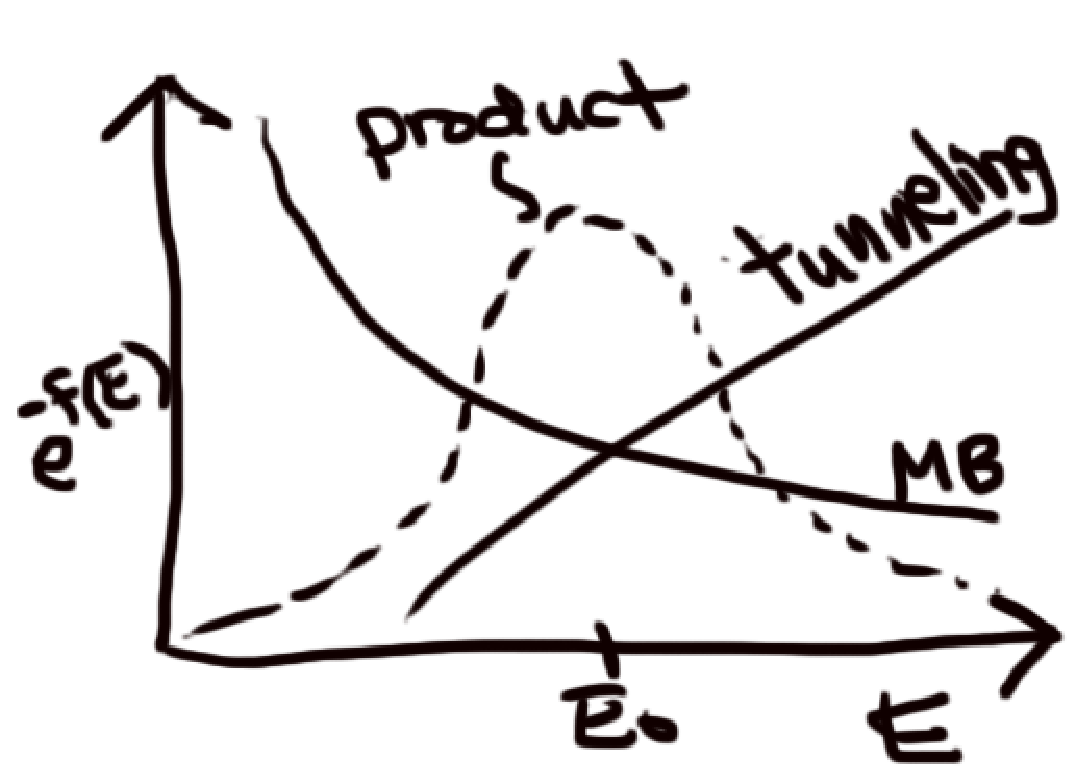
\includegraphics[width=\textwidth/2]{images/fig2.eps}
\label{fig:2}
\caption{}
\end{figure}

Assume $S(E)$ is slowly varying compared to the exponential so that:

\begin{align}
\langle \sigma v\rangle = \lp \frac{2}{kT} \rp^{3/2} \frac{1}{\sqrt{\pi m_{r}}} SI~,I = \int e^{-f(E)}dE~.
\end{align}

$E_{0}$ is the place where $\frac{\delta f}{\delta E} = 0$ i.e., the most probably reaction energy. 

\begin{align}
E_{0} &= \lp \half E_{G}^{1/2}kT\rp^{2/3}~,\textrm{ energy of particles that dominate reactions}\\
E_{0} &\approx (5.7 \textrm{ keV} )Z_{1}^{2/3}Z_{2}^{2/3}T_{7}^{2/3} \lp \frac{m_{r}}{m_{p}} \rp^{1/3}~,T_{7} = T/10^{7}\textrm{K}
\end{align}

At $10^{7}$ K, this roughly corresponds to an energy of 0.87 keV. For the pp chain,

\begin{align}
\underbrace{p + p \ra ...}_{\textrm{at $T \sim 10^{7}$ K}} ~E_{0} \sim 6 \textrm{ keV} \sim 6kT\\
E_{G} \sim 500 \textrm{ keV}~,kT < E_{0} \ll E_{G}\\
S \approx S(E_{0})
\end{align}

We do a Taylor expansion of $f(E)$ to get:

\begin{align}
f(E) &= f(E_{0}) + f' (E_{0})(E - E_{0}) + \half f'' (E_{0})(E-E_{0})^{2}+...\\
I &= e^{-f(E_{0})} \int_{0}^{\infty}e^{-\frac{1}{2} f''(E_{0})(E-E_{0})^{2}}dE\\
f''(E_{0}) &= \frac{3}{4}\frac{E_{G}^{1/2}}{E_{0}^{5/2}} \approx \frac{e^{-f(E_{0})} \sqrt{2\pi}	}{\sqrt{f''(E_{0}}}\\
\underbrace{\langle \sigma v\rangle}_{\textrm{function of $Z_{1},Z_{2},m_{r},T$}} &= \lp \frac{2}{kT}\rp^{3/2}\frac{1}{\sqrt{\pi m_{r}}} S(E_{0})I\\
\Aboxed{\langle \sigma \rangle > &= 2.6 S(E_{0}) \frac{E_{G}^{1/6}}{(kT)^{2/3}\sqrt{m_{r}}} e^{-3(E_{G}/4kT)^{1/3}}}
\end{align}

\section{Energy Generation}

Now, we go back and recall that $r_{12} = n_{1}n_{2}\langle \sigma v\rangle  = $ \# of reactions/vol/time. $Q$ = energy produced by a given reaction.

\begin{align}
\epsilon &= \textrm{erg/s/g generated by reaction } 1 + 2 \ra\\
&= \frac{r_{12}Q}{\rho} = \frac{n_{1}n_{2}\langle \sigma v\rangle Q}{\rho}~,n_{1}=X_{1} \frac{\rho}{m_{1}}
\end{align}

where $X_{1}$ is the fraction of mass in particles of type 1. Now we can write:

\begin{align}
\Aboxed{\epsilon_{12} &= \frac{2.6QS(E_{0})X_{1}X_{2}}{m_{1}m_{2}\sqrt{m_{r}} (kT)^{2/3}} \rho E_{0}^{1/6} e^{-3(E_{G}/4kT)^{1/3}}}
\end{align}

This is a good form because it is not reaction specific. 

\begin{align}
\epsilon &\pt \frac{\rho}{T^{2/3}}e^{-3(E_{G}/4kT)^{1/3}}\\
r &\pt n^{2}\\
\epsilon &\pt \frac{r}{\rho} \pt \rho\\
\Aboxed{\epsilon &\pt \rho^{\alpha}T^{\beta}}~,\alpha=1\textrm{ for a two-body reaction}\\
\ln \epsilon &= \beta \ln T + ...\\
\beta &= \frac{\delta \ln \epsilon}{\delta \ln T} \ra \boxed{ \beta = -\frac{2}{3} + \lp \frac{E_{G}}{4kT} \rp^{1/3}}
\end{align}

\begin{align}
p + p\ra ...~,\textrm{kT}\approx 1\textrm{ keV}\\
E_{G} = 500 \textrm{ keV}~,\beta \approx 4.3\\
\epsilon \pt \rho T^{4.3} \textrm{ near } kT \approx 1\textrm{ keV}
\end{align}

At the center of our sun, $T \sim 10^{7}$ K, $kT=1$ keV, and $\langle \rho\rangle \sim$1 g/cm$^{3}$.

\begin{align}
p + p \ra ... ~,\textrm{ first thing to fuse is the low charge stuff}
\end{align}

For strong interactions, $S \sim $ keV barn $\sim 10^{-33}$ cm$^{2}$ erg. The binding energy per particle released ($Q$) is about 10 MeV. 

\begin{align}
\epsilon \sim 10^{20}\textrm{ ergs/s/g}\\
L = \int \epsilon dM \sim \epsilon M \sim 10^{54}\textrm{ ergs/s } \sim 10^{20} L_{\odot}
\end{align}

We're 20 orders of magnitude off... let's use the weak interaction instead of the strong. 

\chapter{Finishing Fusion}

\begin{center}
\textbf{\begin{huge} October 6, 2011\end{huge}}
\end{center}

\section{FUSION}
\subsection{PP Chain}
We're going into more detail on how to go from $4p \rightarrow ^4He +$ energy, where energy is the KE of particles with a $l \ll R$. There are 2 key ways for the above reaction to occur... one is $p \rightarrow n$, such as beta decay ($n \rightarrow p + e^- + \overline{\nu_e}$). Anything that goes from $ p$ to $n$ has some relation to the weak interaction force. We want the opposite too... where $p + p \rightarrow ^2H + e^+ + \nu_e$. where $^2H$ is Deuterium. 
\begin{align}
S \approx 3.78 \times 10^{-23}~\text{keV barn}
\end{align}

From now on, the ``$\rightarrow$" will be the latter reaction. The pp chain consists of:

\begin{align}
p + p &\rightarrow ^\textrm{$^2$H} + e^+ + \nu_e\\
\textrm{$^2$H} + p &\rightarrow \textrm{$^3$He} + \gamma\\
\textrm{$^3$He} + \textrm{$^3$He} &\rightarrow \textrm{$^4$He} + 2p
\end{align}

Important to note here that the first two reactions must happen twice per 1 of the last one. Since there are no neutrinos, the last two reactions are based on the strong force. This entire cycle produces about 26.7 MeV, but a few \% comes out in the form of neutrinos. \\
Let's find the ergs/s/gram.

\begin{align}
\epsilon \propto \rho T^{-2/3}e^{-3(E_g/4kT)^{1/3}}
\end{align}

Let's recall the $l$ of a reaction, which is $l=\frac{1}{n\sigma}$. $T \approx \frac{l}{v} = \frac{1}{n \sigma v}$. Therefore, the pp step has a $\sigma$ which is must smaller than the other steps. It means almost all the time, most of the reactions in the sun are waiting around for the initial step to happen so that you get $^2H$. The latter steps happen almost instantaneously! The time for the entire cycle (pp chain) is set by the $p + p \rightarrow ^2H + e^+ + \nu_e$. This means we can write:

\begin{align}
\epsilon (\text{energy of entire chain}) = \frac{r_{12} Q}{ \rho} ~,\text{where}~ r_{12}= n_1n_2\langle \sigma v\rangle \\
\\
p + p \rightarrow ... E_g = 1/2 ~\text{MeV}\\
3 (E_g/4kT) = 15.7T_7^{-1/3}\\
\epsilon_{pp}  \propto \rho T^{-2/3} e^{-15.7 T_7^{-1/3}}\\
\epsilon_{pp}  \approx 5 \times 10^5 \frac{\rho X^2}{T_7^{2/3}}e^{-15.7 T_7^{-1/3}}~\text{ergs/s/g}\\
\epsilon \propto \rho T^\beta~,\beta = -2/3 + 5.2T_7^{-1/3}
\end{align}
and in stars like our sun where $T \sim 10^7$ K, $\beta = 4.5$ and $\epsilon \propto T^{4.5}$. Going to use this to estimate the central T of the sun. 

\begin{align}
L &= \int_0^M \epsilon dM_r \approx 0.1 \epsilon_c(r=0)M
\end{align}

use .1 because only 10\% of the mass of the sun contributes to L

\begin{align}
L &= 10^6 \frac{M}{T_7^{2/3}}e^{-15.7T_7^{-1/3}}
\end{align}

Solving for T, we get $T_c \approx 1.5 \times 10^7$K. Our $T_c$ is dependent only on the log of the uncertainty of how much of the sun is fusing. That's one way of going from 4 protons into a He...

\subsection{CNO Cycle}

\begin{align}
\textrm{$^{12}$C}+ p & \rightarrow \textrm{$^{13}$N} + \gamma \\
\textrm{$^{13}$N} & \rightarrow \textrm{$^{13}$C} + e^+ + \nu_e\\
\textrm{$^{13}$C} + p  & \rightarrow \textrm{$^{14}$N} + \gamma\\
\textrm{$^{14}$N} + p & \rightarrow \textrm{$^{15}$O} + \gamma\\
\textrm{$^{15}$O} & \rightarrow \textrm{$^{15}$N} + e^+ + \nu_e\\
\textrm{$^{15}$N}+ p & \rightarrow \textrm{$^{12}$C} + \textrm{$^{4}$He}
\end{align}

Once again, reactions with $\nu_e$ are weak interactions and everything else are strong reactions. In this cycle, line 18 is the slowest step. The first beta decay has a $\lambda$ of 870 sec and the last beta decay has a $\lambda$ of 180 secs. These steps are weak, but still faster than the strong interaction steps. Let's look at how line 18 determines the rate of the CNO cycle. Both the pp chain and the CNO cycle are relevant for generating $ 4p \rightarrow ^4He$. 

\begin{align}
\textrm{$^{14}$N} + p \rightarrow  \textrm{$^{15}$O} + \gamma \\
E_g = 45.7 ~\text{MeV}\\
3 \left( \frac{E_g}{4kT}\right)^{1/3} \approx \frac{70.7}{T_7^{-1/3}}\\
\epsilon_{CNO} & \propto \rho T_7^{-2/3} S_{CNO} e^{-70.6 T_7^{-1/3}}\\
\epsilon_{pp}& \propto \rho T_7^{-2/3} S_{pp}e^{-15.7 T_7^{-1/3}}
\end{align}

$S_{CNO} \sim 10^{24} S_{pp}$, so even if the slowest step in the CNO cycle is a strong process, not a weak process, the extremes cancel each other out. 

\begin{align}
\epsilon &= r_{\text{slowest chain}} \frac{Q}{/\rho}\\
\epsilon_{CNO} &= 4.4 \times 10^{27} \frac{\rho XZ}{T_7^{2/3}} e^{-70.7 T_7 ^{-1/3}}~,\text{where}~ Z = ~\text{mass fraction of heavy elements}
\end{align}

Right at the beginning, stars couldn't use the CNO cycle, but later they are. \\

\begin{align}
\text{For the sun, } &\epsilon_{pp} \propto T^{4.5}\\
\text{CNO:} &\beta = \frac{\delta \ln \epsilon}{\delta \ln T} = -2/3 + 23.6 T_7^{-1/3}~, \epsilon \propto T^\beta\\
& \approx 23~ @~ 10^7 K\\
& \approx 17~@~ 2.7 \times 10^7K\\
& \propto T^{20}
\end{align}

At high T, CNO dominates. At low T, pp dominates. Stars a little more massive that the sun are dominated by CNO, whereas stars a little less massive then than the sun are dominated by the pp chain. \\

In the case of the sun, we have direct evidence to see the effects of fusion. How? Detection of neutrinos! Fusion is dominated in our sun by the pp chain and not the CNO cycle. We also see from neutrinos the approximate central T of the sun. \\

The neutrino matter cross section is dependent on the energy. At the center of the sun, the neutrino $l$ is about $10^9~R_\odot$. They give us the best probe about the center of the sun. \\

Thanks to Ray Davis,
\begin{align}
\textrm{$^{37}$Cl}+ \nu_e \rightarrow \textrm{$^{37}$Ar} + e^-
\end{align}

\chapter{Main Sequence}

\begin{center}
\textbf{\begin{huge} October 11, 2011\end{huge}}
\end{center}

\section{Main Sequence}

Know how to calculate $\epsilon(\rho,T)$ in units of ergs/s/g. Quickly review the major points of the MS:

\begin{align}
\boxed{\frac{dP}{dr}=-\rho \frac{GM_r}{r^2}=-\rho g}\\
P &= P_{gas} + P_{rad} (+ P_{degen})\\
&= \frac{\rho kT}{\mu m_p} + \frac{1}{3}aT^4\\
\boxed{\frac{dM_r}{dr} = 4\pi r^2 \rho}\\
E_{tot} = U/2 = -K, \text{ for NR}\\
E_{tot} \approx 0 , K = -U\text{ for R}
\end{align}

\subsection{Energy Transport (Radiation)}

\begin{align}
F_r = \frac{L_r}{4 \pi r^2} = -\frac{4}{3} \frac{caT^3}{\kappa \rho} \frac{dT}{dR}~,\kappa = \text{ opacity}\\
l = \frac{1}{\kappa \rho} = \frac{1}{n \sigma},\kappa = \frac{\sigma}{m}~,m = \text{ average mass of a particle}\\
\kappa_T,\kappa_{ff},\kappa_{bound~free},\kappa_{H^-},...
\end{align}

\subsection{Energy Transport (Buoyancy)}

Convection sets in if $\frac{ds}{dr} < 0$. Exponentially driven instability is driven by buoyancy of matter. Whether or not its convecting is dependent on the entropy gradient. Another way to put it is:

\begin{align}
\frac{d \ln T}{d \ln P} > \frac{\gamma -1}{\gamma}
\end{align}

We can get away with rough estimates using mixing length to find the work done by the buoyancy force. \\
For convective flux:

\begin{align}
F &= \frac{1}{2}\rho v_c^3\\
&= \frac{1}{2} c_s^3 \Bigl\lvert \frac{H}{c_p} \frac{ds}{dr} \Bigl\lvert ^{3/2}~,
\end{align}

when convection is present, and

\begin{align}
\boxed{\frac{1}{T}\frac{dT}{dr} = \frac{\gamma -1}{\gamma} \frac{d\rho}{dr}}
\end{align}

This is useful for fully convective objects because then $P \pt \rho^\gamma \pt \rho^{5/3}$. This is an example of the $n=3$ polytrope. We can therefore computer $T(r)$ and $\rho(r)$ (relatively) easy.

\subsection{Energy Generation in Stars}


Gravity: KH contraction, at a minimum. 

\begin{align}
\boxed{L = -\frac{1}{2}\frac{dU}{dt}\approx -\frac{GM^2}{R^2} \Bigl\lvert \frac{dR}{dt} \Bigl\lvert}
\end{align}

For the sun, $t_{KH} \approx 30$ million years. This contraction drives $T_c$ up and eventually fusion sets in. $\epsilon(\rho,T,\text{composition})$ is the energy generation by fusion. Fusion is a collisional process and you need both high densities and temperatures for two particles to get close enough to tunnel through their Coulomb Barriers. 

\begin{align}
L \approx \epsilon dM_r = \int_0^R 4 \pi r^2 \rho \epsilon dr
\end{align}

H fusion in the sun lasts about 10$^{10}$ years, which is about 3 orders higher than KH contraction. i.e. fusion is much more important than KH for luminosity. The variables we care about are: $P, \rho, T , L_r , M_r$ and the equations are: HE, Equation of State, $dM_r = 4\pi r^2 \rho$, energy transport, and energy generation. While these equations are good, we need boundary conditions/initial conditions. If you specify the mass and initial composition of a star, that determines \textit{everything} $(T_c,T_{eff},\rho,R,L,T(r),P(r),...)$. For KH contraction, we could calculate $R(M, t)$ and $L(M, t)$.

\chapter{Understanding Stellar Evolution}

\begin{center}
\textbf{\begin{huge} October 13, 2011\end{huge}}
\end{center}

The balance we're interested in is:

\begin{align}
L_{fusion} &\approx L_{rad/conv}\\
	& + 	\text{HE}\rightarrow\text{main sequence}
\end{align}

For stars of $M \leq M_\odot$, supported by $P_{gas}$, pp chain fusion, and $\kappa \sim \kappa_{ff}$. And if $\gamma$ carry energy out, $L_{rad} \propto \frac{ M^{5.5} }{\sqrt{R}}$. Estimating $L_{fusion} = \epsilon_c M$. In the case of pp fusion, $\epsilon_{pp} \propto \rho T_c^{4/5}$ where $kT_c \sim \frac{GM \mu m_p}{R}$. \\

\begin{align}
L_{fusion} \pt \frac{M^{6/5}}{R^{7.5}}
\end{align}

If you change the $L$ of the star, $T$ and $\rho$ must change to accommodate. In steady state:

\begin{align}
L_{fusion} \pt \frac{M^{6/5}}{R^{7.5}} & \pt \frac{ M^{5.5} }{\sqrt{R}}\\
R & \pt M^{1/7}\\
T_c &\pt M^{6/7}\\
L & \pt M^{5.4}\\
L & \pt T_{eff}^4~ \pt 4\pi R^2\sigma T^4~, \text{but R dependence is so weak it's estimated to be constant}
\end{align}

\begin{align}
M \uparrow~,T_c \uparrow \sim M^{6/7}\\
\epsilon_{pp} \pt T^{4.5}~, \epsilon_{CNO} \pt T^{20}
\end{align}

Stars that are more massive than the sun are very $T$ dependent. \\

For $M \geq M_\odot$: $\kappa \sim \kappa_T \sim$ constant. $\gamma$ still dominate $E$ transport. CNO cycle is dominant mechanism and $P_{gas}$ dominates. $L_{rad} \pt M^3$.

\begin{align}
L_{fusion}&  = \int \epsilon_{CNO} dM_r\\
 & \sim \epsilon_{CNO}M~, \epsilon_{CNO} \pt \rho T_c^{20}\\
 \epsilon_{CNO} \pt \frac{M^{21}}{R^{23}}\\
 L_{fusion} \sim L_{rad}\\
  \frac{M^{22}}{R^{23}} \pt M^3\\
  R \pt M^{19/23} \pt M^{.8}\\
  T_c \pt M^{.2}
\end{align}

\begin{align}
L & = 4 \pi R^2 \sigma T_{eff}^4\\
L & \pt R^2 T_{eff}^4\\
R^2  & \pt M^{1.6} \pt L^{1/2}\\
L & \pt M^3\\
   & \pt L^{1/2}T_{eff}^4\\
L^{1/2} & \pt T_{eff}^4\\
L & \pt T_{eff}^8\\
T_{eff} & \pt M^{3/8}
\end{align}

A huge change in L corresponds to a small change in $T$. Only for stars with masses slightly more than the sun. \\

For $M \geq 1.2 M_\odot$, they have convective cores and $\gamma$ transport energy on outer part of star. Reverse of our sun. Convection sets in if $\frac{ds}{dr} < 0$. $\frac{ds}{dr}$ is implied by $\gamma$ transport of energy. You can then use radiative diffusion equation to see if $\frac{ds}{dr}<0$. i.e. Convection sets in if $\frac{d \ln T}{d \ln P} > \frac{\gamma -1}{\gamma}$. $\gamma$ is the one for photons, not of the particles convecting. 

\begin{align}
\frac{d \ln T}{d \ln P}  = \frac{1}{4} \frac{P}{P_{rad}}\frac{L}{L_{edd}}\frac{L_r/L}{M_r/M}~,L_{edd} = \frac{4 \pi G M_c}{\kappa}
\end{align}

$P$ is the total pressure. This tells us convection sets in if $\frac{1}{4} \frac{P}{P_{rad}}\frac{L}{L_{edd}}\frac{L_r/L}{M_r/M} > \frac{2}{5}$. Recall for CNO, $\epsilon \pt \rho T^\beta$. At almost all $r$, $L_r \approx L$. For CNO-dominated stars, only 1\% of star's mass fuses. TINY! It's this enormous flux that originates so close so the core that it drives convection. $\frac{M_r}{M} < \frac{5}{8} \frac{P}{P_{rad}}\frac{L}{L_{edd}}$, then convection sets in. We're interested where $P \approx P_{rad}$. We want to know $\frac{P}{P_{rad}}$ and $\frac{L}{L_{edd}}$. $L \pt M^3$ and $L_{EDD} \pt M$ so $\frac{L}{L_{edd}} = 4.5 \times 10^{-5} \left( \frac{M}{M_\odot} \right)^2$. \\

In the sun, $r \sim 0 \rightarrow .5 R_\odot$, $\frac{P_{gas}}{P_{rad}} \sim 3000$.

\begin{align}
P_{gas} &\pt \rho T \pt \frac{M^2}{R^4}\\
P_{rad}& = \frac{1}{3}a T^4 \pt \frac{M^4}{R^4}\\
\frac{P_{gas}}{P_{rad}} &\pt M^{-2}\\
\frac{P_{gas}}{P_{rad}} &\approx 3000 \left( \frac{M}{M_\odot} \right)^{-2}
\end{align}

Convection sets in if $\frac{M_r}{M} \leq 0.1$. \\

Lifetime of MS star $\approx \frac{E_{nuc}}{L}$. 

\begin{align}
L = L_\odot \left( \frac{M}{M_\odot} \right)^{3.5}\\
E_{nuc} &= N_p E\\
&  \approx  .1 \frac{M}{m_p}~\times 7 ~\text{MeV}\\
\frac{E_{nuc}}{L} \approx 10^{10} \left( \frac{M}{M_\odot} \right)^{-2.5}
\end{align}

ANY star with a mass less than .85$M_\odot$ is still fusing after 13.7 billion years. For $M \sim 30 M_\odot$, $t_{MS}$ is about $10^6$ years. Massive stars live and die where they are born. 
\chapter{QM Effects in Stars}

\begin{center}
\textbf{\begin{huge} October 18, 2011\end{huge}}
\end{center}

\section{Min and Max Masses of Stars}

A star is an object held together by it's own gravity; undergoes H fusion into He. Doesn't matter if it's fused in the past, it's still a star, just at a different phase in it's life. In the present day universe, stars have $M$ between $.08 M_\odot  \leq M \leq 100-200 M_\odot$. The fact that stars under $.08M_\odot$ don't undergo fusion is well understood, due to the QM nature of stars. The fact that stars above $100-200 M_\odot$ don't fuse, however, isn't well understood. Best guess it has something to with $P$ dominated by $P_{rad}$.

\subsection{Lower Limit}

Th lower limit is placed based on the QM properties of the gas in stars. We've treated the gas in stars as an ideal, classical gas. $P  = nkT + \frac{1}{3}aT^4$. What is required for the aforementioned equation to be valid? 1) QM degeneracy $P$ is small, 2) at typical distance, not interacting with itself. QM nature is important when:

\begin{align}
\lambda \gtrsim \text{ distance between particles} \sim n^{-3}\\
p_{th} = mv_{th} \approx \sqrt{mkT}\\
\lambda = \frac{h}{p} = \frac{h}{\sqrt{mkT}}\\
\end{align}

The QM nature is important if $\lambda \geq n^{-3} $. $n \geq \lp \frac{mkT}{h^2} \rp^{3/2}$. 

\begin{align}
n_Q &\equiv \text{ quantum density}\\
&= \lp \frac{2 \pi m k T}{h^2} \rp ^{3/2} = n_Q(T)\\
n &\geq n_Q~,\text{ then QM is important}
\end{align}

If $n_q \pt m^{3/2}$, then the first particles you have to worry about are the electrons, not the protons. Electrons have a lower mass, but what about photons? \\

At the center of the sun, density of electrons is actually close to the quantum density. So what we've been doing so far has been wrong? If we think about stars of different masses, we need to look at how the $T$ and $\rho$ change with $M$. 

\begin{align}
R \pt M^{3/4}\\
T_C \pt \frac{M}{R} \pt M^{1/4} \downarrow \text{ as } M \downarrow~, n_Q \downarrow \text{ too}\\
\rho \pt \frac{M}{R^3} \pt \frac{M}{M^{9/4}} \pt M^{-5/4}~, n \uparrow \text{ as } M \downarrow\\
\end{align}

QM becomes increasingly important for low mass stars. It's the electrons we worry about, specifically. Distribution function of particles isn't really MB, but something more general.\\

\begin{align}
n(p)= \frac{2/h^3}{e^{(E_p - \mu)/kT} \pm 1}~, E_p = p^2 c^2 + m^2 c^4,\mu = \text{ chemical potential} = \frac{\delta E}{ \delta N} \Bigl\lvert_{S,V}
\end{align}

$\pm$ relates to: "$+$" obeys Fermi-Dirac Statistics and "$-$" obeys Bose-Einstein Statistics. We want Fermi statistics because electrons lie there. $n(p)$ is the number density defined to be: 

\begin{align}
n= \int d^3 p \cdot n(p)~,
\end{align}

where $n(p)$ is the number of particles per unit volume in $d^3x \pt d^3p$. Real space and in momentum space. Now we're going to focus on Fermions...

\subsection{Fermions}

\begin{align}
n(p)= \frac{2/h^3}{e^{(E_p - \mu)/kT} + 1}
\end{align}

Let's consider a fully degenerate gas. i.e. QM nature is very very important. This is at the limit $n \gg n_Q$ where $T \rightarrow 0$. What is the limit of the distribution function as $T \rightarrow 0$? 

\begin{align}
e^{\pm \text{ big \#}}
\end{align}

$n(p) \simeq 0 $ if $E_p > \mu$ and $n(p) \simeq \frac{2}{h^3} $ if $E_p < \mu$. This is only in the QM limit though. But! Stars never reach $T = 0$, so what do we really mean? When we say the T is 0, we mean the thermal energy is small compared to something. More precisely, $\mu \gg kT$. \\

We can just calculate the number density $n$ of fermions, $n = \int n(p) \times d^3p$. This is either an integral of 0 or a constant. Define: $p_F$ as the Fermi Momentum

\begin{align}
p_F = p \text{ such that }E_p = \mu
\end{align}

Then, 

\begin{align}
n &= \int_{0}^{p_F} \frac{2}{h^3}d^3p\\
&= \frac{8 \pi}{h^3} \int_0^{p_F} p^2 dp\\
&= \frac{8 \pi}{3h^3} p_F^3\\
\Aboxed{p_F &= \lp \frac{3h^3}{8 \pi} \rp^{1/3} n^{1/3}}~,\text{ this is true in both NR and R limits}
\end{align}

Let's assume NR fermions:

\begin{align}
E_p &= \frac{1}{2}mv^2 = \frac{p^2}{2m}\\
E_F &= \frac{p_F^2}{2m}\\
\Aboxed{&= \lp \frac{3h^3}{8 \pi} \rp ^{2/3} \frac{n^{2/3}}{2m} }
\end{align}

This can also be described as $\mu$. $\boxed{\mu = E_F}$. No matter how close to $T=0$ you get, particles will still move!

\begin{list}{}{}
\item gas density $n$
\item typical dist between particles $\sim n^{-1/3}$
\end{list}

If $\lambda \geq n^{-1/3}$, particles seem to blur together. But the P.E.P says that particles needs to be in separate discrete states. This blurring isn't possible for fermions that obey the P.E.P. If you obey the P.E.P, you have to have a $\lambda \leq n^{-1/3}$, even if $T \rightarrow 0$. As you get closer to $T \rightarrow 0$, then $\lambda \geq n^{-1/3}$, but at some point, P.E.P. forces $\lambda \leq n^{-1/3}$. 

\begin{align}
\frac{h}{p}\sim n^{-1/3} \rightarrow p \sim hn^{-1/3} \sim p_F
\end{align}

The $p_F$ is largely determined by $\lambda$. Whether particles are R or NR is irrelevant, they can still be QM in both situations. If we assume things are NR, $E_F \sim \frac{p_F^2}{2m		} \sim \frac{h^2}{2m} n^{2/3} \equiv \mu$. The flux you radiate doesn't care about the Fermi nature of the electrons. When we say $F = aT^4$, we mean $T$ to be $T$, not kinetic energy, not thermal energy, just $T$. With QM, we're saying that even with a low $T$, we can still have a high $p$ and $E$. \\

What we really want to understand is the structure of low mass stars. What is the pressure produced by these particles? This is what's going to compete with gas or radiation pressure. Remember

\begin{align}
P &= \frac{2}{3} \epsilon\text{ for NR} \\
P &= \frac{1}{3} \epsilon \text{ for R}
\end{align}

Our guess would be for the NR case:

\begin{align}
P  &\sim n E_F~,\text{ number of particles per unit volume time energy per particle}\\
P &\sim \frac{h^2}{2m}n^{5/3}
\end{align}

\begin{align}
\epsilon &= \int \frac{p^2}{2m}n(p) d^3p\\
&= \int_0^{p_F} \frac{p^2}{mh^3}4 \pi p^2 dp \\
&= \frac{4 \pi}{mh^3} \int_0^{p_F} p^4 dp\\
\Aboxed{\epsilon &= \frac{4 \pi}{5} \lp \frac{3}{8 \pi} \rp^{5/3} \frac{h^2 n^{5/3}}{m}}
\end{align}

\begin{align}
\Aboxed{P &= \frac{h^2}{5m} \lp \frac{3}{8 \pi} \rp^{2/3} n^{5/3}}~\text{ NR QM degeneracy pressure of fermions}\\
&\pt \frac{n^{5/3}}{m}~,\text{ lowest mass particles dominates pressure (in our case, $e^-$)}\\
&\pt \frac{n^{5/3}}{m}~,\text{ $n=3/2$ polytrope!}
\end{align}

Since $P \pt n^{5/3}$ it doesn't mean the star is convective although the opposite is true. It's totally unrelated. Elliot thinks. We assumed a NR gas of fermions, now how about R? $p_F$ is so large that the velocity approaches the speed of light. Can't use $P = \frac{2}{3} \epsilon$, must use $P = \frac{1}{3} \epsilon$.

\begin{align}
\epsilon \sim n \times p_F c~,p_fc = E_F\\
p_F \sim hn^{1/3}\\
P _{\text{R Degenerate Gas}}&\sim hn^{4/3}c\\
&\sim \frac{hc}{4} \lp \frac{3}{8 \pi} \rp^{1/3} n^{4/3}~,\text{ only depends on $p$, not $p$ and $m$.}
\end{align}

This is an example of a $n=3$ polytrope. 

\chapter{Mass of Stars}

\begin{center}
\textbf{\begin{huge} October 25, 2011\end{huge}}
\end{center}

\section{Minimum Mass of Stars $M_\star \gtrsim .08 M_\odot$}

If you have gas with an inter-particle spacing $a$, and if it's a bunch of Fermions, then quantum mechanically, we require that the $\lambda$ be less than the inter-particle spacing. This can be violated when:

\begin{align}
\lambda &\leq a\\
\frac{h}{p_{th}} &\sim \frac{h}{\sqrt{kTm}}
\end{align}

There is a finite momentum such that at $T=0$, there is still energy.

\begin{align}
\frac{h}{p} \sim a \sim n^{-1/3}
\end{align}

This relates to the Fermi momentum $p_F \sim hn^{-1/3}$. This makes no assumption about the relativistic properties of the gas. Associated with the Fermi momentum and the case of a NR gas,

\begin{align}
E_F = \frac{p_F^2}{2m	} \sim \frac{h^2 n^{2/3}}{2m}
\end{align}

Lastly, because the particles have a certain momentum, they collide and exchange momentum, exerting a force and thus a pressure. 

\begin{align}
P &\sim \text{ energy volume}^{-1}\\
&\sim nE_F
\end{align}

For a NR quantum gas, we have a pressure: $\dfrac{h^2n^{5/3}}{2m}$. If you do it another way with integrals and stuff, you get: 

\begin{align}
P = \frac{h^2}{5m} \lp \frac{3}{8 \pi} \rp^{2/3} n^{5/3}~,P \pt \rho^{5/3}~,n=\sfrac{3}{2}\text{ polytrope}
\end{align}

We get this by integrating the momentum distribution which is a straight line until $p_F$ by where it drops to 0. Recall, $\mu = \lp \frac{\delta E}{\delta N} \rp_{S,V} = E_F$. For a classical gas, $\mu$ changes with $kT$. Quantum mechanically, you adds particles with $E_F$. For R QM gases:

\begin{align}
E = pc\\
E_F = p_F c\sim hn^{1/3}c\\
\Aboxed{P &\sim hn^{4/3}c}\\
\Aboxed{&\sim E_F n}~,P \pt \rho^{4/3}~,n=3\text{ polytrope}
\end{align}

\section{Types of Ideal Gases}

There exists two types of ideal gases, Classical and QM. One way to tell apart is whether or not $\lambda$ is comparable to inter-particle spacing. Another is whether the quantum density is comparable to the gas density. Put another way, $n > n_Q$ is QM, $n < n_Q$ is classical. You can also compare:

\begin{align}
nkT &\sim P_{degen}\\
E_F& \sim kT
\end{align}

Where does $T$ come in for the deBr\"oglie Wavelength? It comes in from $\lambda = \frac{h}{p_{th}}$, where $p_{th}$ is a function of $T$.\\

As a star of mass $M \downarrow, n\uparrow, T \downarrow, n_Q \downarrow$, which pushes you more towards the limit where QM is important. 

\section{Low Mass Object}

We know that these are fully convective, where for fully convective objects:

\begin{align}
P_c = .5 GM^{2/3}\rho_c^{4/3}
\end{align}

which comes from:

\begin{align}
\frac{dP}{dr} &= -\rho \frac{GM_r}{r^2}\\
P_c &\sim \rho \frac{GM}{R}~,\rho \sim \frac{M}{R^3}~,R \sim \lp \frac{M}{\rho} \rp^{1/3}\\
P_c &\sim GM^{2/3}\rho^{4/3}~,P_c \text{ is from a gas of radiation}
\end{align}

Now,

\begin{align}
P_c &= P_{gas} + P_{degen}\\
&= \underbrace{nkT}_{\text{from protons}} + \underbrace{\frac{h^2}{5m} \lp \frac{3}{8 \pi} \rp^{2/3} n^{5/3}}_{\text{from electrons}}\\
&= n_p kT + \frac{h^2}{5m} \lp \frac{3}{8 \pi} \rp^{2/3} n_e^{5/3}\\
&= \frac{\rho kT}{\mu m_p} + \frac{h^2}{5m} \lp \frac{3}{8 \pi} \rp^{2/3} \lp  \frac{\rho}{\mu_e m_p}\rp^{5/3}\\
&= \frac{\rho_c kT}{\mu m_p} + \frac{h^2}{5m} \lp \frac{3}{8 \pi} \rp^{2/3} \lp  \frac{\rho_c}{\mu_e m_p}\rp^{5/3}\\
&= 0.5 GM^{2/3} \rho_c^{4/3}
\end{align}

This tells us that $\rho_c T_c \pt \rho_c ^{4/3}M^{2/3}$ classically to get $T_c \pt \rho_c^{1/3}M^{2/3}$. Now, we want to include the $P_{degen}$ to find $T_c$ given $\rho_c$. 

\begin{align}
T_c = 6 \times 10^6 \text{ K} \mfrac^{2/3}\rho_c^{1/3} - 10^5 \text{ K} \rho_c^{2/3}
\end{align}

As you increase $\rho_c$, $T_c \ra 0$ at some $\rho_c$. Line 24 is the $T_c$ required for HE given $M$ and $\rho_c$. At some central density, it's large enough to provide all the pressure needed to support the star. The star is fully supported by degeneracy pressure and there is no gas pressure. For larger central densities, it's nonphysical. If $T_c = 0$, there is a unique $\rho_c$ so that $P_{degen} =$ gravity. 

\begin{align}
\rho_c^{5/3} &\pt M^{2/3} \rho_c^{4/3}\\
\rho_c^{1/3} &\pt M^{2/3}\\
\rho_c &\pt M^2~,\text{ unique $\rho_c$ given $M$}\\
&\pt \frac{M}{R^3}\\
R &\pt M^{-1/3}~,\text{ unique $R$ given $M$ for deg. pressure support}
\end{align}

For stars undergoing KH contraction,

\begin{align}
\rho_c \uparrow, T_c \uparrow\\
P_{gas} \uparrow\\
P_{degen} \uparrow
\end{align}

To stop this contraction, the $T_c$ gets high enough so that you get fusion. OR the star finds another way to support itself. The $P_{degen}$ can get large enough so that it becomes comparable to HE and you stop contracting without ever having to fuse. There's a battle within the star between $T$ and $\rho_c$. Either you get hot enough so that fusion sets in or your $\rho_c$ gets high enough so that $P_{degen}$ supports the star.

\section{That One Graph that Looks like an LN plot but that touches down at the X axis}

There is a $T_{MAX}$ an object can have supported by $P_{gas} + P_{degen}$.

\begin{align}
\frac{dT_c}{d\rho_c} = 0\\
8 \times 10^7 \text{ K} \mfrac^{4/3}
\end{align}

If $T_{MAX}$ is large enough, fusion sets in and you become a star. If $T_{MAX}$ is too small, there is no fusion and you are supported by degen. pressure, resulting in a brown dwarf or a giant planet. \\

For fusion to stop KH contraction, you need:

\begin{align}
\underbrace{L_{conv}}_{\text{energy leaving star}} = \underbrace{L_{fusion}}_{\text{energy generated by fusion}}\\
L_{fusion} \sim \epsilon_{pp}M\\
T = 10^7 \text{ K}~, L \sim .01 L_\odot \rho \mfrac\\
T = 10^6 \text{ K}~, L \sim 10^{-9} L_\odot \rho \mfrac\\
T = 2 \times 10^6 \text{ K}~, L \sim 10^{-6} L_\odot \rho \mfrac
\end{align}

Basically, you need $T_c \gtrsim 2 \times 10^6$ K for fusion of H to stop KH contraction. If you set $2 \times 10^6 K = T_{MAX} = 8 \times10^7 \text{ K} \mfrac^{4/3}$, you get $M \leq .06 M_\odot, T_c < 2 \times 10^6 $ K and it is supported by deg. pressure because it never got hot enough to fuse. On the other hand, $M \geq .06 M_\odot \ra T_c > 2 \times 10^6$ K, fusion sets in, stops KH contraction, and is now on the MS. \\

Detailed calculations give $M \gtrsim .08 M_\odot$ are stars, and $M \lesssim .08 M_\odot$ are not. 

%
%the circle is where degen presureis about the same as gravity. the plot is for jupiter
%

\begin{list}{$\circ$}{}
\item $D= \dfrac{n_D}{d_p} \sim 3 \times 10^{-5}$
\item $Li = \dfrac{n_{Li}}{n_p} \sim 3 \times 10^{-10}$
\end{list}

But they fuse before H. Why? Let's look at the reactions:

\begin{align}
p + D &\ra \textrm{$^{3}$He} + \gamma\\
E_G &= 655 \text{ KeV}\\
p + \textrm{$^{7}$Li} & \ra \textrm{$^{4}$He} + \textrm{$^{4}$He}\\
E_G &= 7.7 \text{ MeV}\\
p + p &\ra ...\\
E_G &= 508 \text{ KeV}
\end{align}

It's because their $S$ value is so large. Why? The reactions are strong reactions. There's a little tiny D and Li Main Sequence. 

\section{Max Mass of Stars (Quickly)}

Observationally, it looks like (at least in nearby galaxies) that there aren't stars with $M \geq 100 \ra 300M_\odot$. This is subtle though, since in a model you could come up with a star with $1000 M_\odot$, we just don't think they're stable. In particular these are $P_{Rad}$ supported, so they have a $\gamma = \sfrac{4}{3}$ and their $E_{tot} = 0$. It may be the case that these stars form, but they are SOOO unstable that any perturbation and they oscillate out of control. But hey, it's all speculation. 

\chapter{Stellar Atmospheres and Spectra}

\begin{center}
\textbf{\begin{huge} October 27, 2011\end{huge}}
\end{center}

\section{Stellar Classification}

Photosphere is where $l \simeq H$ which implies $l = \frac{1}{\kappa \rho} \approx \frac{kT}{mg}$. This then turns into $n \approx \frac{g}{kT\kappa}, P \approx\frac{g}{\kappa}$. For our sun, 
\begin{list}{$\circ$}{}
\item $T_{eff}= 5800$ K
\item  $n = 10^{17} $ cm$^{-3}\sim 10^{-3} n_\oplus$
\item $P \approx 10^5 $ dyne cm$^{-2} = 0.1$ atm
\end{list}  

For a MS Star,
\begin{list}{$\circ$}{}
\item $T_{eff} = 5800$ K $\mfrac^{3/8} \ra n(M), P(M)$
\item $M \approx 0.1 M_\odot, T_{eff} \sim 3000$ K
\item $M \approx 100M_\odot, T_{eff} \sim 30,000$ K
\end{list}  

\begin{list}{$\circ$}{}
\item O B A F G K M L T (L \& T have $T_{eff} \sim 1000 - 1500$ K and are dominated by molecular lines and bands)
\end{list}

In a nutshell, the $M$ gives us the $T_{eff}$ which will in turn give us the spectra. This is understood as a consequence of thermal equilibrium in the atmospheres of stars. Imagine an atom/molecule with energy levels $E_i$ and $E_j$:

\begin{align}
\frac{N_j}{N_i} = \frac{g_j}{g_i}e^{-(E_j - E_i)/kT}
\end{align}

Are the atoms in this atmosphere ionized or neutral and how does it depend on temperature? This we will understand through the Saha Equation which deals with ionization equilibrium. You have ionization (bound electron + photon = free electron) and recombination (electron + proton = bound neutral hydrogen atom) in a gas. What deals with changes in particles? $\mu$.... oh no.

\section{Chemical Potential and Thermal Equilibrium}

\begin{align}
dE = TdS + PdV - \mu dN\\
P,T,\mu: \text{macroscopic thermodynamic properties of a gas}\\
P = \lp \frac{\delta E}{\delta V} \rp_{S,N}\\
\mu = \lp \frac{\delta E}{\delta N} \rp_{S,V}\\
T = \lp \frac{\delta E}{\delta S} \rp_{V,N}
\end{align}

Approach thermal equilibrium via changes in:

\begin{list}{$\circ$}{}
\item heat/temp (changes in thermal energy)
\item pressure (changes in volume)
\item chemical potential (changes in \# or type of particle)
\end{list}

Say you have a box with $N_1,V_1,E_1$ and $N_2,V_2,E_2$ on another side with a separator in between. If you exchange energy between the particles (exchange of heat), then thermodynamic equilibrium is the temperatures equal each other. If the boundary is permeable, then the pressures become equal to each other. If you can exchange the number of types of particles, such as the ionization and recombination process, then in thermal equilibrium, the chemical potentials become equal. \\

For our purposes, what this means is that if you have reactions that convert:

\begin{align}
A + B \ra C + D\\
\underbrace{C + D \ra A + B}_{\text{ approach thermal equilibrium}}\\
\mu(A) + \mu(B) = \mu(C) + \mu(D)
\end{align}

\section{H Fusion}

\begin{align}
4 H \ra ^4He~,\text{ no opposite reaction and thus no thermal equilibrium describable with $\mu$}
\end{align}

But we can work with:
\begin{align}
e^- + p \ra H + \gamma~.
\end{align}

\begin{align}
\underbrace{\text{\# of recombinations per vol per unit time} = \text{\# of ionizations per vol per unit time}}_{\text{after long enough time so that both directions have happened}}
\end{align}

This can be described as:
\begin{align}
\mu(e^-) + \mu(p) = \mu(H) + \mu(\gamma)
\end{align}

\section{How to Calculate $\mu$}

$e^-,p,H,...$ in the atmospheres of stars can be described as a classical, ideal gas. What is the $\mu$ of a classical, ideal gas? We know how to calculate it for a degenerate gas ($\mu = E_F$), but not for classical yet. We have to go back to the distribution function that describes particles as a function of momentum. 

\begin{align}
n(p) &= \frac{g}{h^3} \frac{1}{e^{(E_p - \mu)/kT} \pm 1}~,\text{ $g$ is a constant related to spin states}\\
n(p) &= \text{ density in $p-$space}\\
``+" &= \text{ Fermions}\\
``-" &= \text{ Bosons}
\end{align}

If it's classical, should mean that we don't care either fermions or bosons. we would \textit{GUESS} that the exponential is $\gg 1$. Then,

\begin{align}
n(p) &= \frac{g}{h^3}e ^{-(E_p - \mu)/kT}\\
E_p^2 &= p^2c^2 +  m^2c^4~.
\end{align}

However, line 18 isn't completely classical because there's still an $h$ in the equation. Recall the classical limit is when $\lambda \ll n^{-1/3}$ or $n \ll n_Q = \lp \frac{2 \pi m kT}{h^2} \rp^{3/2}$.

\subsection{NR Gas}

\begin{align}
E_p^2 &= mc^2\lp 1 + \frac{p^2c^2}{mc^4} \rp^{1/2}\\
E_p &= mc^2 \lp 1 + \frac{p^2}{2m} \frac{1}{mc^2} \rp\\
E_p &= \underbrace{mc^2}_{\text{ rest mass}} + \underbrace{\frac{p^2}{2m}}_{\text{ kinetic}}
\end{align}

\begin{align}
\mu + E_F \pt n^{2/3}\\
n &= \int n(p) d^3p\\
&= 4 \pi \int p^2 dp n(p)\\
&= \frac{4 \pi g}{h^3}  \in p^2 e^{-(mc^2 + \frac{p^2}{2m} - \mu)/kT} dp\\
&= \frac{4 \pi g}{h^3} e^{(\mu -mc^2)/kT} \underbrace{\int  p^2 e^{-\frac{p^2}{2mkT}} dp}_{(2mkT)^{3/2} \frac{\sqrt{\pi}}{4}}\\
\Aboxed{n &= g e^{(\mu - mc^2)/kT} \lp \frac{2 \pi mkT}{h^2} \rp^{3/2}}\\
\Aboxed{n &= n_Q g e^{(\mu - mc^2)/kT}}\\
e^{(mc^2 - \mu)/kT} = g\frac{n_Q}{n} \gg 1 ~, \text{ for classical}\\
n \ll n_Q \ra e^{(E_p - \mu)/kT} \gg 1
\end{align}

Now we'll solve for $\mu$

\begin{align}
\boxed{\mu = mc^2 - kT \ln \lp \frac{gn_Q}{n} \rp} ~,\text{ $\mu$ for a classical, NR ideal gas, }kT \gg E_F
\end{align}

For a degenerate gas, $p_F \sim hn^{1/3}$, $E_F \sim \frac{h^2 n^{2/3}}{m} \equiv \mu$ of a degenerate NR gas. For this, $kT \ll E_F$. \\

We wanted to understand ionization balance in stars (focusing on $H$) which is described by:

\begin{align}
\mu(p) + \mu(e^-) = \mu(H) + \underbrace{\mu(\gamma)}_{\mu = 0}
\end{align}

To actually implement this:

\begin{align}
\mu(p) &= m_pc^2 - kT\ln \lp \frac{gn_{Q,p}}{n_p} \rp\\
\mu(e^-) &= m_ec^2 - kT\ln \lp \frac{gn_{Q,e}}{n_e} \rp\\
\mu(H) &= m_Hc^2 - kT\ln \lp \frac{gn_{Q,H}}{n_h} \rp~,\text{ where $n_H$ is the density of neutral hydrogen}\\
m_Hc^2 &= m_pc^2 + m_ec^2 - \chi~,\chi = \text{ binding energy of $e^-$ and $p$ in atom}
\end{align}

\begin{align}
\mu(H) &= \mu(p) + \mu(e^-)\\
m_pc^2 + m_ec^2 - \chi - kT \ln \lp \frac{gn_{Q,H}}{n_H} \rp &= m_pc^2+m_ec^2 - kT\ln \lp \frac{g_e n_{Q,e}}{n_e} \rp -  kT\ln \lp \frac{g_p n_{Q,p}}{n_p} \rp\\
\frac{n_e  n_p}{n_H} &= \frac{g_eg_p}{g_H}n_{Q,e} e^{-\chi/kT}~,\text{ Saha Equation for ionization balance}
\end{align}


\chapter{Stellar Spectra Continued}

\begin{center}
\textbf{\begin{huge} November 1, 2011\end{huge}}
\end{center}

\section{Saha Equation}

Recall, 

\begin{align}
\text{\# of ionizations} = \text{\# of atoms neutral vs \# ionized}
\end{align}

How do we describe $\mu(H) = \mu(p) + \mu(e^-)$ mathematically? For a classical, NR gas, 

\begin{align}
\boxed{\mu = mc^2 -kT \ln \lp \frac{gn_Q}{n} \rp}~.
\end{align}

Since the temperatures we care about sets the thermal energy to be around the binding energy of $H$, we can't ignore it and must include it in 

\begin{align}
m_Hc^2 &= m_pc^2 + m_ec^2 - \chi~.
\end{align}

\begin{align}
-\frac{\chi}{kT} &= \ln \lp \frac{g_H n_{Q,H}n_en_p}{n_Hn_{Q,e}n_{Q,p}g_eg_p}\rp\\
n_Q &= \lp \frac{2 \pi mkT}{h^2} \rp^{3/2}\\
n_{Q,H} &= n_{Q,p}\\
\Aboxed{\frac{n_en_p}{n_H} &= \frac{g_eg_p}{g_H}n_{Q,e}e^{-\chi / kT}}~,\text{ Saha Equation of $H$}\\
n_H: \text{ $H$ in the ground state, $\chi = 13.6$ eV}
\end{align}

At what $T$ is $H$ half-ionized?

\begin{align}
n_e &= n_p= n_H\\
\frac{n_en_p}{n_H} &= n_H~\text{ for the ground state of $H$, $g_H = 2$}\\
n_H &= \lp \frac{2 \pi m_e kT}{h^2} \rp^{3/2} e^{-\chi /kT}\\
T_4 = T / 10^4 \text{ K}\\
\chi /kT = \frac{15.77}{T_4}\\
13.6 \text{ eV} \ra T = 1.577 \times 10^5 \text{ K}\\
n_H &= \lp \frac{2 \pi m_e kT}{h^2} \rp^{3/2}  e^{-15.77/T_4}~,~T \text{ at which $H$ is half-ionized given $n$}
\end{align}

For the sun,

\begin{align}
\frac{1}{\kappa \rho} = \frac{kT}{mg} \ra n\approx 10^{12} \text{ cm}^{-3}\\
1 \approx \frac{3 \times 10^4}{n_{17}}T_4^{3/2} e^{-15.77 /kT}~,n_{17} = n/10^{17}\\
T \approx 1.5 \times 10^4 \text{ K for $H$ to be half-ionized at $n = 10^{17}$ cm$^{-3}$}
\end{align}

$H$ is half-ionized at $kT \sim 0.1 \chi$! Even though the $T$ is well below the ionization $T$ of $H$, it's because there are many more free electron states. There are many QM states of a free electron at $10^4$ K, creating a bias even though there's an energy wall you have to go through. This  $kT \sim 0.1 \chi$ proves to e a very good rule of thumb for stars. \\

He is ionized a about 24.6 eV and is half-ionized at around $kT \sim 0.1 \chi, T \approx 1 \times 10^4$ K. Na has an ionization energy of 5.14 eV, needing $T > 6000$ K for it to be ionized. \\

The Saha Equation however doesn't work very well (quantitatively not applicable) in the interior of stars... and there's two reasons for that. In low mass stars, degeneracy pressure dominates core pressure and $n \sim n_Q$ and thus you can't treat it as a classical gas. Also, the spacing between particles is now less than the B\"ohr radius for densities above 1 gm cm$^{-3}$. There's a version of the Saha Equation for degenerate gases, but not for overlapping energy levels, it's too complicated.

\section{Masses and What's What }

3 types of elements:
\begin{list}{$\circ$}{}
\item Noble gases: He and Ne, $\chi \sim 25$ eV, ionized at around $T \sim 30,000$ K
\item H, C, N, O $\chi \sim 10$ eV, ionized around $T \sim 10^4$ K
\item Metals: Na, K, ... $\chi \sim 6$ eV, ionized around $T \sim 5000$ K
\end{list} 
These energies are just to strip off the first electron, btw. 

\begin{center}
\begin{tabular}{lccc}
\hline
Mass ($M_\odot$)&Class&$T_{eff}$ (K)&What's ionized\\ \hline
100&O& $ \sim 30,000$&He II, all else ionized\\ \hline
10&B& $\sim 20,000$&He neutral\\ \hline
2.5&A&$ \sim 9,000$&H neutral\\ \hline
1&G& $\sim 6,000$&neutral metals\\ \hline
0.1&M&$\sim 3,000$&all neutral (almost)\\ \hline
\end{tabular}
\end{center}

\section{Balmer Lines of $H$}

The Balmer lines correspond to $n=2 \ra n=3,4,5,...$ and are important because they correspond to the optical lines of $H$. To go from $n=1$ to $n=2$ takes 10.2 eV, just to know. What determines whether or not you'll see a Balmer line is dependent on how many electrons there are in the $n=2$ state. i.e., the $\frac{n_{n=2}}{n_H}$ which determines the strength of the line. 

\begin{align}
\frac{n_{n=2}}{n_{n=1}} = 4e^{-\Delta E /kT}
\end{align}

How is it that even though in the best case scenario, where 1 out of 100,000 electrons have the energy needed to emit a Balmer Line, that line is sufficiently strong in stars? To have an observable line, the $l$ due to the atomic transition is $\ll$ the $l$ of other photons in the spectrum. This is basically the condition for stars to have a ``strong" line. 

\begin{align}
l &= \frac{1}{n \sigma}\\
l &= \frac{1}{n_{n=2} \sigma_{\text{line}}}~,\text{ for a Balmer line}\\
l_{\text{other photons}} &= \frac{1}{n_{tot} \sigma_{cont}}~,\sigma_{cont} \sim \sigma_T
\end{align}

Strong Balmer line requires:

\begin{align}
n_{n=2}\sigma_{\text{line}} &> n_{tot}\sigma_T\\
\frac{n_{n=2}}{n_{tot}} &> \frac{\sigma_T}{\sigma_{\text{line}}}
\end{align}

For Balmer lines, $\sigma_{\text{line}} \sim a_0^2 \sim 10^{-16}$ cm$^2$ and $\sigma_T \sim 6.65 \times 10^{-25}$ cm$^2$. Strong line requires:

\begin{align}
\frac{n_{n=2}}{n_{tot}} \geq 10^{-8}
\end{align}

Even though the number of electrons in the $n=2$ state is so small, the $\sigma_{\text{line}} $ is so large. So far, we've understood that the spectrum of a star depends primarily on its $T_{eff}$ and also it's composition. There is one other thing it depends on, and that's the $R$ of a star. On the MS, $M \ra T \ra L \ra T_{eff}$, but off the MS, two stars can have the same $T_{eff}$ and have different $R$ (giants). Where does this come into the problem?

\begin{align}
T_{eff} \\
n_{ph} &: \frac{1}{\kappa \rho} = \frac{kT_{eff}}{mg}\\
n &\approx \frac{g}{\kappa kT_{eff}}\\
&\approx \frac{GM}{R^2 \kappa kT_{eff}}
\end{align}

For $M = M_\odot$, $T_{eff} = 5800$ K and $R = 100R_\odot$ (giant). This then corresponds to $n_{ph} \sim 10^{13}$ cm$^{-3}$ which changes the spectrum (subtly). T at which $H$ is half-ionized: $1.5 \times 10^4$ K at $n=10^{17}$ cm$^{-3}$ and $8000$ K at $n = 10^{13}$ cm$^{-3}$. 
\chapter{Stellar Evolution}

\begin{center}
\textbf{\begin{huge} November 03, 2011\end{huge}}
\end{center}

\section{Stellar Evolution}

\begin{align}
t_{MS} = \frac{E_{NUC}}{L} \approx 10^{10} \mfrac^{-2.5} \textrm{ years}
\end{align}

On the Main Sequence, the star undergoes fusion from H into He in the core where then the properties of the star change in time. Radiative transport of energy dominates where $\sigma = \sigma_T$. $L \pt M^3 \mu^4 \mu_e$. The important thing to note is that on the MS, the luminosity of the star increases as it ages. \\

At time = 0, $X = .75, Y = .25, \mu = 0.6, \mu_e=1$ which then turns into pure He, $\mu_e=2, \mu = \sfrac{4}{3} \ra \frac{L(t_{MS})}{L(t=0)} \approx 40$, which arises just from the change in composition of the star. But we know the entire star doesn't convert into He, except for fully convective star where there's a lot of mixing. To do this correctly...\\
$0.1 M:$ H $\ra$ He (core) with properties: $X = 0.65, Y = 0.35, \mu = 0.64, \frac{L(t_{MS})}{L(t=0)} = 1.4$, which means at the end of its life cycle, it'll be 40\% brighter. For us, this corresponds to a change in $T$ of about 60$^{\circ}$F. This gives rise to the issue that earlier in the sun's lifetime it was significantly cooler and thus the earth might have had problems evolving life. Buuuut this is stellar physics not astrobiology or whatever. Why Fahrenheit all of a sudden? Don't worry about it.\\

Let's start with a nice picture of a star with a He core and a H shell where the mass in the He core is about 0.1$M_{tot}$. Since this core isn't fusing, it's undergoing KH contraction. Core contraction causes $T$ to go up, causing fusion of heavier elements which then runs out, contracts, ad infinitum (At least until Fe or something). This cycle involves simultaneously the $T_c$ and $\rho_c$ both going up. What stops this cycle? It depends on two pieces of key physics:\\

\begin{list}{$\circ$}{}
\item An object supported by electron degeneracy pressure has a maximum mass (Chandrasekhar mass, about 1.4 $\ms$). We'll prove this later. 
\end{list}

\noindent If the mass of the star's core is greater than $M_{ch}$, then the degeneracy pressure can't stop contraction. 

\begin{list}{$\circ$}{}
\item $T_{max} \approx 8 \times 10^7$ K $\mfrac^{4/3}$ of a star with gas pressure and NR degeneracy pressure.
\end{list}

\noindent i.e. if a star is supported by NR degeneracy pressure, you can't be hotter than the $T$ above. Imposing the two conditions, then you get:

\begin{align}
M < M_{ch} \ra T_{max} < 2 \times 10^8\textrm{ K}~.
\end{align}

\noindent This means you can't fuse to arbitrarily high Z. In particular, things that have $M<M_{ch}$ can only fuse He $\ra$ C,O but no higher. To fuse Mg, you need $T \approx 10^9$ K or so. 

\section{What is the End Fate of a Star?}

... and it's dependency on it's initial mass?\\

We have to take into account the difference of mass between final mass and initial mass. Towards the end of a star's life (esp. massive stars), a lot of mass is lost. Roughly, stars with $M_i \lesssim 8 \ms$, they end up with a core with a mass less than $M_{ch}$, becoming supported by electron degeneracy, which stops the cycle of KH contraction. These are usually C/O composition. This is a white dwarf, in particular, a C/O white dwarf. This is exactly the same argument as to why brown dwarves exist. The change of mass, $\sim 6\ms$, is blown away by powerful stellar winds. Some dwarves continue to fuse, but most stop at C/O. Stars with $M < 0.5 \ms$, you never fuse He. The MS lifetime of a $0.5 \ms$ is longer than the age of the universe... but we still see them anyways. 

\subsection{$M_i > 8\ms$}

These end with a core heavier than $M_{ch}$ so they can't be supported by electron degeneracy. This also means there is no maximum temperature. Using V.T and some other stuff, $T \pt \rho^{1/3}$  and if one increases, so does the other. Eventually you fuse all the heavier elements up to iron. Iron is important because they're the tightest bound atomic nuclei. Once you hit Iron, fusion is no longer a source of energy. Now, there's nothing to maintain the $T$. It's too massive to be supported by electron degeneracy... leaving $P_{gas}$ and $P_{rad}$, but they both depend on $T$. You run into the case where you have no pressure support and the star collapses. The collapse produces either a neutron star or a black hole and an explosion. The core may be a NS or BH, but the explosion blows away the outer part of the star. This is a supernova. FYI, the in falling material is moving $\sim c$. Stellar evolution is a little complicated in that you have to keep separate what the core is doing and what the outer part of the star is doing. 

\section{End of the MS}

He core, surrounded mostly by H and other stuff. Imagine H fusion shuts off (in the center) which make the star contracts. This makes the $\rho_c,T_c \uparrow$ as well as the H envelope $\rho,T \uparrow$. You end up with a He core and a H fusing shell surrounded by the rest of the envelope. The core has to get pretty hot for it to fuse the next step but the shell only has to get a little hotter to fuse. The core is still contracting, resulting in the $L_{shell} \uparrow$. Out in the envelope, photons are carrying the energy, carrying out the $L_{rad} = L_\odot \mfrac^3$. At some point, this $L_{shell}$ is greater than the energy photons can carry out in the envelope. Now, you're going to start pushing stuff out, driving convection. Once the entire envelope becomes convective, it can carry energy out pretty effectively.\\

Now the star is a giant with the outer parts of the star convecting. The image here is a He core, H shell fusion, and big puffy convective envelope. On the MS, what happens if there was a little extra fusion in the center of the sun? It would expand and $T \downarrow$, but that doesn't happen here. In that scenario, the core and envelope are doing the same thing, which isn't happening here. Basically, the core is forcing the physics of the entire star. There's nothing stopping the core contracting (runaway) and there's no ``safety valve" of the MS. This contraction for the sun is extremely fast (on stellar scales) on about a $t_{KH}$ time scale $\sim 10^7$ years. If you look on the HR diagram, you'll see a lot of stars at the giant stage, then it's pretty empty until you hit the white dwarf area. An interesting note is that during the giant stage the $T_{eff}$ gets to about 3000-4000 K and scrapes the Hayashi Line.\\

Eventually, the core stops contracting and you can either have He Fusion or be supported by degeneracy pressure. Let's continue imagining a core undergoing He fusion and H fusion in shell where the $L_{shell}$ continues to increase in time. As H in the shell goes to He, the mass of the He core increases, causing the $T_{shell}$ to go up, causing $L_{shell}$ to increase. At this stage, the star is moving up the Hayashi Line (i.e. ``up the giant branch"). The reason the $L \uparrow$ is thanks to convection. As $L = 4 \pi R^2T_{eff}^2$ increases with $T_{eff}$ staying roughly constant, the radius goes up. Eventually, a bunch of H is fused and then He fusions begins. A star steadily fusing He has a relatively long lifetime; it's like a He MS. Lower mass stars have degenerate cores and undergoes degenerate He fusion. In this scenario, there is no ``safety valve" and with deg. He fusion, $P \pt \rho^{5/3}$, leading to runaway He fusion (He flash) puffing up the star quickly. \\

Any stars $0.5 \ms$ and higher go through the He fusion stage pretty predictably. Going into this later. 

\chapter{He Fusion}

\begin{center}
\textbf{\begin{huge} November 08, 2011\end{huge}}
\end{center}

\section{He Fusion}

After stars fuse on the MS, stars finish fusing H and He fusion begins, shell fusion starts, outer parts are expanded and become fully convective. Once the star hits the Hayashi Line, it goes up the giant branch because the energy can be carried out by convection. Eventually the contraction of the core stops, either through deg pressure dominating or fusion of higher mass elements.\\
He fusion is special because the natural fusion processes you might think of are:

\begin{align}
\textrm{$^{4}$He}+\textrm{$^{4}$He} &\ra \textrm{$^{8}$Be}~,\lambda = 3 \times 10^{-16} \textrm{ s}~,\textrm{ unstable!}\\
\textrm{$^{4}$He} + \textrm{p} &\ra \textrm{stuff}\\
\textrm{$^{8}$Be} &\ra \textrm{$^{4}$He} + \textrm{$^{4}$He}
\end{align}

This should look like the balance between ionization and recombination.\\

Let's look closely at the first step, $\textrm{$^{4}$He}+\textrm{$^{4}$He} \ra \textrm{$^{8}$Be}$. This is an endothermic reaction because it requires energy, about 92 keV. It's a little strange because it doesn't directly release energy. It just means that Be is a little less bound than 2 He nuclei. What does it take to get this reaction going? First guess might be that $E_{thm} \geq$ 92 keV. Another guess involves:

\begin{align}
E_0 &= \lp \frac{E_G (kT)^2}{4} \rp^{1/3}~,
\end{align}

where $E_0$ is the energy of particles on the MB tail that produce the most fusion reactions.

\begin{align}
E_G &\simeq 1 \frac{m_r}{m_p}Z_1^2Z_2^2\textrm{ MeV}\\
E_0& \geq 92 \textrm{ keV}\\
E_0 &= 84 T_8^{2/3}\textrm{ keV}
\end{align}

For $T \gtrsim 10^8$ K, $\textrm{$^{4}$He}+\textrm{$^{4}$He} \ra \textrm{$^{8}$Be}$ can happen, but it immediately decays. This is an example where we can calculate the properties of fusion in a star with thermodynamic equilibrium. We can approach TE when:

\begin{align}
\textrm{\# decays of Be}& \ra \textrm{\# of fusion}\\
2\mu(^4\textrm{He}) &= \mu(^8\textrm{Be})~.
\end{align}

There is a net amount of Be in the star even though it's very unstable. Now that there's a finite amount of Be...

\begin{align}
\textrm{$^{8}$Be} + \textrm{$^{4}$He} &\ra \textrm{$^{12}$C}\\
\textrm{$^{12}$C}+ \textrm{$^{4}$He}&\ra \textrm{$^{16}$O}
\end{align}

Recall, He fusion involves fusion to C/O so it makes sense. Line 10 gives off an energy of about 7.367 MeV. Imagine a C nucleus has a bunch of energy levels. Line 10 was guessed to be a resonant reaction (thanks, Hoyle), which means that the energy of $\textrm{$^{8}$Be} + \textrm{$^{4}$He}$ combine to be almost exactly the energy of one of the nuclear excited states of C (7.65 MeV). Thus, this reaction is \textit{preferential}. You actually need:

\begin{align}
E_0 &\gtrsim 7.65 - 7.37\textrm{ MeV in order for this reaction to actually go}\\
&\gtrsim 290 \textrm{ keV}\\
&\gtrsim 150 T_8^{2/3} \textrm{ keV}~, T \gtrsim \textrm{ few $10^8$ K}
\end{align}

This reaction actually wins out over fusion to the ground state. We just used the (or rather, Hoyle did) anthropic principle in that since we see so much C and O, it must be happening more in stars than we can explain. So what it's telling us is that over a few $10^8$ K, we can get Be fusion and a little more T, we can get to an excited state of C. Unfortunately, that excited state is unstable. Most of the time,

\begin{align}
\textrm{$^{12}$C$^*$} \ra \textrm{$^{4}$He}+ \textrm{$^{8}$Be}
\end{align}

But every once in a while, C doesn't decay by spitting a He nucleus out, it decays by nuclei rearranging itself and spitting out a photon,

\begin{align}
^{12}\textrm{C}^* \ra \textrm{$^{12}$C}+ \gamma~, \gamma = 7.65 \textrm{ MeV.}
\end{align}

The half life for the above reaction is about $1.8 \times 10^{-13}$ sec and this is where we get most of our C that we know and love. Now, how do I describe this step quantitatively? 

\begin{align}
\mu(\textrm{$^{4}$He}) + \mu(\textrm{$^{8}$Be})=\mu(\textrm{$^{12}$C$^*$} )
\end{align}

You have to take into account $\mu$ instead of $r=n_1n_2\langle \sigma v\rangle $ because the latter doesn't take into account most of the C$^*$ decaying back into He and Be. Now, we have:

\begin{align}
\textrm{$^{4}$He} + \textrm{$^{4}$He} &\leftrightarrow \textrm{$^{8}$Be} \\
\textrm{$^{8}$Be}  + \textrm{$^{4}$He} &\leftrightarrow \textrm{$^{12}$C$^*$}\\
2 \mu(^4\textrm{He}) &= \mu(^8\textrm{Be})\\
\mu(^8\textrm{He}) + \mu(^4\textrm{He}) &= \mu(^{12}\textrm{C}^*)\\
\Aboxed{3\mu(^4\textrm{He}) &= \mu(^{12}\textrm{C}^*)}\\
^4\textrm{He} + \textrm{$^{4}$He} + \textrm{$^{4}$He} &\leftrightarrow \textrm{$^{12}$C$^*$}~,\textrm{ this is called the ``triple $\alpha$" process.}
\end{align}

\begin{align}
m_{\textrm{excited C}}c^2 &= 3m_{\textrm{He}}c^2 + \Delta E~, \Delta E = 379 \textrm{ keV}
\end{align}

$\Delta E$ is the combined energy needed to push each individual reaction, basically. The energy of the photon is what supports the star during He fusion.\\

\begin{align}
3\mu(^4\textrm{He}) &= \mu(^{12}\textrm{C}^*)\\
-kT\ln \lp \frac{g_4 n_{Q,4}}{n_4} \rp^3 &= \Delta E - kT \ln \lp \frac{g_{12}n_{Q,12}}{n_{12^*}} \rp~,\textrm{ 4 corresponds to He, 12 corresponds to C}\\
\frac{g_4^3 n_{Q,4}^3 n_{12^*}}{n_4^3 g_{12} n_{Q,12}} &= e^{-\Delta E /kT}~,g_4 = g_{12} = 1\\
n_Q &= \lp \frac{2 \pi mkT}{h^2} \rp^{3/2}\\
n_{Q,12} &= 3^{3/2}n_{Q,4}\\
\Aboxed{\frac{n_{12^*}}{n_4^3} &= 3^{3/2} \lp \frac{h^2}{8 \pi m_p kT} \rp^3 e^{-\Delta E/kT}}~, m_{He} = 4m_p
\end{align}

But why are the degeneracies 1? Eliot doesn't know :( When we had H recombination, at high T, ionization won and things were broken apart. Conversely, at low T, things were neutral. Here, at high T, the reactions favor $^{12}$C$^*$ and at low T, $^4$He is favored. The big difference is that it requires energy to fuse the latter. To make excited C \textit{requires} energy. In H fusion, it was $-\chi$; here it's $+\Delta E$. 

\begin{align}
n_4 &= \frac{\rho}{4m_p}~,Y = \textrm{ overall He mass fraction}\\
n_{12^*} &=\frac{Y^3 \rho^3}{(4m_p)^3}3^{3/2} \lp \frac{h^2}{8 \pi m_p kT} \rp^3 e^{-44/T_8}~,\frac{\Delta E}{kT} = \frac{44}{T_8}
\end{align}

Recall $\lambda$ of $n_{12^*}$ is $1.8 \times 10^{-13}$ sec. How do we represent this quantitatively? 

\begin{align}
\frac{dn_{12}}{dt} &= \frac{n_{12^*}}{\lambda}
\end{align}

This is the \# of $^{12}$C in the ground state created per unit time per unit volume. The energy generated by unit fusion is:

\begin{align}
\underbrace{\epsilon}_{\textrm{ergs/s/g}} &= \frac{\frac{dn_{12}}{dt} \cdot \underbrace{E}_{7.65\textrm{ MeV}}}{\rho}\\
\Aboxed{\epsilon &= 5.4 \times 10^{11} \frac{\rho^2 Y^3}{T_8^3} e^{-44/T_8}\textrm{ ergs/s/g}}
\end{align}

This looks a lot more like TE because it is such an argument that gives us the rate at which C is created. 

\begin{align}
\epsilon \pt \rho^\alpha T^\beta~,\alpha =2
\end{align}

$\alpha=2$ because we have 3 things turning into 1 thing, whereas before we had 2 things turn into 1 thing. This is effectively a 3-body process and thus the rate of reactions goes something like $\frac{\rho^3}{\rho} = \rho^2$.

\begin{align}
\epsilon \pt \rho^\alpha T^\beta~,\beta = -3 +\frac{44}{T_8}
\end{align}

The T sensitivity isn't sensitive to tunneling anymore, it's sensitive to TE.

\begin{align}
\textrm{$^{4}$He} + \textrm{$^{4}$He} + \textrm{$^{4}$He} &\ra \textrm{$^{12}$C}\\
\textrm{$^{12}$C}+ \textrm{$^{4}$He}& \ra \textrm{$^{16}$O}\\
T\sim 10^8\textrm{ K}
\end{align}

Bottom line is you get C and O in vaguely similar amounts.

\section{Back to the Bigger Picture}
Let's put this in the context of stellar evolution. Now we're at the He core fusing with a H shell fusing. This is a long-lived phase in the life of a star. This is analogous to the H-MS, now called the Horizontal Branch (HB). What happens now? This is finished when He has been converted into C/O or for higher M stars, Mg, Ne, etc. Imagine a C/O core, a He shell, and an even bigger H shell. The core contracts and you get He fusion in the shell, generating more and more E, going into expanding layers of the star, resulting in a giant. Once it's expanded to reach the Hayashi Line, the outer part becomes fully convective again and it goes up the HL again. This is the Asymptotic Giant Branch (ASB), similar in observational appearance to the RGB. In detail, there are small differences due to composition changes, but for the most part they behave the same.\\

There's 2 possibilities now...
\begin{list}{$^\circ$}{}
\item Star supported by $e^-$ degeneracy pressure
\item C/O fusion starts
\end{list}

What's special for lower mass stars ($M_i \lesssim 8\ms$) is that the core has a mass less than the Chandrasekhar mass so it automatically becomes supported by degeneracy pressure. It's important to note that most of the mass lost is on the RGB and AGB in very short-lived phases ($10^4 \sim 10^5$ years). There are 2 bits of physics to note:
\begin{list}{$^\circ$}{}
\item He shell fusion is unstable 
\item Dust forms in the atmosphere of the star. The $L_* > L_{EDD,dust} = L_{dust}$.
\end{list}
Blowing mass out reveals a hot white dwarf and it \textit{looks} like it's getting hotter, but it's really not. These WDs that ionize shells of gas are named planetary nebula even though they have nothing to do with planets. Thank pre-HST astrophysicists. 

\chapter{White Dwarfs}

\begin{center}
\textbf{\begin{huge} November 10, 2011\end{huge}}
\end{center}

\section{Non-Relativistic White Dwarfs}

Supported by NR electron degeneracy pressure.

\begin{align}
P &=  \frac{h^2}{5m_e}\lp \frac{3}{8 \pi} \rp^{2/3} n_e^{5/3}\\
P &\sim E_F n~,E_F = \frac{p_F^2}{2m}~,p_F \sim hn^{1/3}
\end{align}

\begin{align}
n_e &= \frac{\rho}{\mu_e m_p}\\
P &= K\rho^{5/3}~,K = \frac{h^2}{5m_e} \lp \frac{3}{8\pi} \rp^{2/3} \lp \frac{1}{\mu_e m_p}\rp^{5/3}
\end{align}

For a $n=\sfrac{3}{2}\textrm{ polytrope}$,

\begin{align}
P_c &= 0.77 \frac{GM^2}{R^4}\\
\rho_c &= 6\langle \rho\rangle = \frac{GM}{\frac{4}{3} \pi R^3} = \frac{9}{2\pi} \frac{M}{R^3}\\
P_c &= K\rho_c^{5/3}\\
0.77 \frac{GM^2}{R^4} &= K \lp \frac{9}{2\pi}\rp^{5/3} \frac{M^{5/3}}{R^5}\\
\Aboxed{R &\pt M^{-1/3}}
\end{align}

For degenerate objects, more massive objects are physically smaller.

\begin{align}
R &= 2.34 \frac{K}{G} M^{-1/3}\\
\Aboxed{&= 0.04R_\odot \mfrac^{-1/3}\mu_e^{-5/3}}
\end{align}

So for C/O, 

\begin{align}
\mu_e &= 2\\
\Aboxed{R &\simeq 0.013 R_\odot \mfrac^{-1/3} \lp \frac{\mu_e}{2} \rp^{-5/3}}
\end{align}
For $M\sim M_\odot$, $R \sim 10^9$ cm $\sim R_\oplus$.

We assume the electrons were NR in the above equations. We know that the $p_F\sim n^{1/3}h$.
\begin{align}
\langle \rho \rangle = \frac{M}{\frac{4}{3} \pi R^3}\approx 6 \times 10^5 \mfrac^2\textrm{ gm cm}^{-3}\\
\rho_c = 6\langle \rho \rangle \approx 4 \times 10^6 \mfrac^2 \textrm{ gm cm}^{-3}
\end{align}
\begin{align}
p_F \sim 3 \times 10^{-17} \mfrac^{2/3} \textrm{ gm cm s}^{-1}
\end{align}
We can use the simple relation $p_F = v_em_e$ to get $v_e \approx 4 \times 10^{10} \mfrac^{2/3}$ cm/s. WHAAAT. As $M$ increases, $v_e$ increases and $e^-$ become increasingly relativistic. 

\section{Relativistic White Dwarf Stars}

\begin{align}
P &\sim E_F n\\
E_F &= \underbrace{\frac{p_F^2}{2m}}_{\textrm{non-relativistic}} \textrm{ or } \underbrace{p_Fc}_{\textrm{relativistic}}
\end{align}

If $e^-$ are completely relativistic, $E_F \gg m_ec^2$ and so we can ignore rest mass energy. 

\begin{align}
E_F &= p_Fc\\
p &\sim hcn_e^{4/3}\\
\Aboxed{P &= \frac{hc}{4} \lp \frac{3}{8\pi}\rp^{1/3}n_e^{4/3}}
\end{align}

Now let's do it again!

\begin{align}
n_e& = \frac{\rho}{\mu_e m_p}\\
P &= K\rho^{4/3}~,K = \frac{hc}{4} \lp \frac{3}{8\pi} \rp^{1/3} \lp \frac{1}{\mu_e m_p}\rp^{4/3}
\end{align}
This is a $n=3$ polytrope.
\begin{align}
P_c &= 11 \frac{GM^2}{R^4}\\
\rho_c &= 54.2 \langle \rho \rangle \\
&= 12.9 \frac{M}{R^3}\\
P_c &= K\rho_c^{4/3}\\
11 \frac{GM^2}{R^4} &= K30\frac{M^{4/3}}{R^4}\\
\Aboxed{M &\approx 4.6 \lp \frac{K}{G} \rp^{3/2}}\\
M &\approx 0.2 \frac{(hc)^{3/2}}{(\mu_e m_p)^2G^{3/2}}\\
\Aboxed{M &\approx 1.45 \lp \frac{\mu_e}{2} \rp^{-2} \ms = M_{ch}}
\end{align}

But what does this mean? Let's look at Hydrostatic Equilibrium:

\begin{align}
\frac{dP}{dr} &= -\rho \frac{GM_r}{r^2}~,\rho \sim \frac{M}{R^3}\\
P &\sim \frac{GM^2}{R^4}\\
P &\pt \rho^{4/3} \pt \frac{M^{4/3}}{R^4}
\end{align}

For a NR electron gas:
\begin{align}
P &\pt \rho^{5/3} \pt \frac{M^{5/3}}{R^5}\\
\frac{M^{5/3}}{R^5}&\pt \frac{M^2}{R^4}\\
R &\pt M^{-1/3}
\end{align}
\begin{align}
\frac{M^{4/3}}{R^4} &\pt \frac{M^2}{R^4}~M\uparrow\textrm{ gravity $>$ pressure}
\end{align}

So as $M \uparrow$, $R\downarrow$ in Hydrostatic Equilibrium. As M gets larger and larger, there will be some maximum mass above which we can't have pressure balance gravity. Hydrostatic Equilibrium will fail. $M_{ch}$ is the maximum mass for objects supported by electron degeneracy pressure. 

\section{The Life of a White Dwarf}

White Dwarf stars are born hot and luminous but fade away in time. There's a reservoir of thermal energy that it's born with that it radiates slowly over time. Energy transport  in a white dwarf is dominated by thermal conduction (also true in neutron stars). This is different from stars like the sun where energy transport by photons is much much more effective than conduction.

\begin{align}
F &= -\kappa \nabla T~,\kappa = \frac{1}{3}vl\frac{dU}{dT}~, \frac{dU}{dT}= \textrm{specific heat of particles}
\end{align}

For a normal star, $v = v_{th} = \sqrt{\frac{kT}{m_e}}$
\begin{align}
\frac{dU}{dT} \sim nk~,U = \frac{3}{2}nkT~,l=l_c\textrm{ coulomb scattering}
\end{align}
but in a WD,
\begin{align}
v &\sim \frac{p_F}{m_e} \sim c\\
U &= nE_f~,\textrm{ but if it was the case, then } \frac{dU}{dT} = 0
\end{align}
Instead, we have to add a term to $nE_F$ to correct:
\begin{align}
U &\sim nE_F + \theta (kT)^2\\
\frac{dU}{dT} &\approx nk \underbrace{\frac{kT}{E_F}}_{\ll1}
\end{align}

Scattering in a white dwarf is still dominated by $l_c$, but the energy of an electron is no longer dependent on temperature. We used to have $\frac{e^2}{b} \sim E_i$, where in the classical case, $E_i = kT$ and in the white dwarf case, $E_i = E_F$. 

\begin{align}
\Aboxed{\sigma_c &\sim \pi b^2 \sim \frac{ \pi e^4}{E_F^2}}
\end{align}

In a white dwarf where the $E_F \gg kT$, $\sigma_c \ll $ normal star and therefore $l_c = \frac{1}{n\sigma_c} \gg $ normal star. Putting this all together,

\begin{align}
\kappa_{\textrm{degen}} = 10^3 \cdot T_8^{-3/2}\kappa_{\textrm{classical}}(T)
\end{align}

This is why electron conduction is much more important than photon energy transport. 

\begin{align}
\kappa_{\textrm{degen}} \approx \frac{k^2h^3Tn_i}{Z_i^232e^4m_e^2}~,n_i = \textrm{ ion-$e^-$ scattering}
\end{align}

Let's imagine a $T$ profile just after fusion: 

%Insert plot here 

It'll try to make temperature uniform and after a little while, the $T_c$ is pretty much constant. The time to become isothermal is roughly $10^6 \sim 10^7$ years. Over time, the white dwarf cools by radiating initial thermal energy away. We just said that the energy of an electron is proportional to $E_F\lp 1 + \lp \frac{kT}{E_F}\rp^2 \rp$. C/O isn't degenerate, so there, $E = kT$. The important note is that it's mostly the thermal energy of the ions that's being radiated. 

\begin{align}
L_{\textrm{WD}} \approx 5L_\odot \mfrac \lp \frac{T_c}{10^8 \textrm{ K}} \rp^{7/2}~
\end{align}

Remember we use $T_8$ because it's about what the C/O core is born at.
\begin{align}
\frac{T_c}{10^8\textrm{ K}} &\approx \lp \frac{t}{10^6\textrm{ yr}} \rp\\
L &\approx 5 L_\odot \mfrac \lp \frac{t}{10^6 \textrm{ yr}} \rp^{-7/5}
\end{align}
\begin{align}
L &= 4\pi R^2 \sigma T_{eff}^4\\
T_{eff} &\approx 58,000 \lp \frac{L}{L_\odot} \rp^{1/4} \textrm{ K}\\
\Aboxed{T_{eff} &\pt t^{-0.35}}
\end{align}

A 1 Gyr white dwarf would have:
\begin{align}
L &\sim 3 \times 10^{-4} L_\odot\\
T_{eff} &= 9000\textrm{ K}
\end{align}

A 10 Gyr white dwarf would have:
\begin{align}
L &\sim 10^{-5} L_\odot\\
T_{eff} &= 3000\textrm{ K}
\end{align}


\chapter{Evolution of Massive Stars}

\begin{center}
\textbf{\begin{huge} November 15, 2011\end{huge}}
\end{center}

\section{Intro to Massive Stars}

White dwarf stars are usually comprised mostly of C/O. He fusion has occurred, leading to an abundance of C/O. Not $^{12}$C +  $^{12}$C $\ra$ $^{20}$Ne + $\alpha$ which requires temps of about $10^9$ K. Recall, if a star has a $M < M_{ch}$, the core contracts and is supported by electron degeneracy. This is the central reason why most white dwarf stars are C/O. They just don't get hot enough to fuse C into heavier elements. 

\subsection{Massive Stars}

\begin{align}
M_{\textrm{core}} &> M_{ch}\\
P_c &= P_{gas} + P_{degen}~,P_c \sim GM^{2/3}\rho^{4/3}\textrm{ (HE)}
\end{align}

for stars supported by electron degeneracy pressure, then the electron degeneracy pressure is $\pt \rho^{5/3}$. For stars above $M_{ch}$, $P_{deg} \pt \rho_c^{4/3}$. i.e., 
\begin{align}
M > M_{ch} \ra P_{degen} < P_c \forall \rho_c~.
\end{align}

In the case of massive stars,
\begin{align}
\underbrace{P_c}_{\pt \rho_c^{4/3}} &= \underbrace{P_{gas}}_{\pt \rho_cT_c\ra T_c \pt \rho_c^{1/3}} + \underbrace{P_{degen}}_{\pt T_c^4}
\end{align}

As the star contracts, $T_c \uparrow$, leading into fusion of heavier elements, cycling back to $T_c \uparrow$. Once you get to $^{56}$Fe, there is no way for fusion of heavier elements to provide energy. Fusion dies, electron degeneracy pressure fades out and the star collapses in on itself. This is the fate of stars with $M > M_{ch}$. Basically, once you're above $M_{ch}$, the only support is high $T$ which when you run out of fusion, will collapse. It's good to note that the time to go from Si to Fe is about a day while going from H to He takes a much longer time. The reason for this is as you get hotter, the dominant way the star loses energy is no longer through radiating photons, but now through radiating neutrinos. This happens at around C fusion. Since neutrinos leave the star really easily, energy is carried out much more effectively, accelerating the fusion process. 
\section{Importance of $\nu$'s}
These neutrinos are not neutrinos from nuclear reactions. These are thermal neutrinos, simply produced from high $T$. 
\begin{align}
L_{\textrm{fusion}} &= L_{\textrm{rad}}
\end{align}
But for C fusion and later, 
\begin{align}
L_{\textrm{fusion}} = L_{\nu}~.
\end{align}

They're very good at moving energy away since $\sigma_{\nu} \sim 10^{-44} \lp \frac{E_{\nu}}{m_ec^2} \rp^2$. $m_ec^2 = kT \ra T \sim 10^9$ K. %
%
%\begin{align}
%\frac{l}{R}~,\frac{M}{m_p R^3}
%\end{align}
As long as the radius is less than 30 km or so, the $l_\nu$ is longer than the radius and can leave very quickly. But where do they come form? Also, why are they different from fusion neutrinos? 

\subsection{Positron Number Density}%Thermal $\nu$ Production}
\begin{align}
e^- + e^+ \ra \nu_e + \overline{\nu_e} \textrm{ (rare), most of the time it's photons}
\end{align}

But where do the positrons come from? The answer is $\gamma + \gamma \ra e^- + e^+$. For this to have \textbf{ANY} chance, $m_ec^2 \sim 511$ keV $\sim 6 \times 10^9$ K. If I want to calculate how many positrons there are in a star, then I have use use $\mu$. 
\begin{align}
\gamma + \gamma &\ra e^- + e^+\\
e^- + e^+ &\ra \gamma + \gamma\\
\mu(e^+) + \mu(e^-) &= 2\mu(\gamma) = 0\\
\Aboxed{\mu(e^+) &= -\mu(e^-)}
\end{align}

We can use this to calculate $n_{e^+}$. We're going to assume non-relativistic and non-degenerate. 
\begin{align}
m_ec^2 - kT\ln \lp \frac{gn_Q}{n_{e^+}} \rp &= -m_ec^2 + kT\ln \lp \frac{gn_Q}{n_{e^-}} \rp\\
2m_ec^2 &= kT \ln \lp \frac{g^2n_Q^2}{n_{e^-} n_{e^+}} \rp\\
n_{e^-}  n_{e^+} &= g^2n_Q^2e^{-2m_ec^2/kT}
\end{align}

Plugging in numbers, 
\begin{align}
n_{e^-}  n_{e^+} &= 2 \times 10^{58} T_9^3 e^{-11.9/T_9}\textrm{ cm}^{-6}
\end{align}

But to find the $n_{e^+}$, we need to know $n_{e^-}$. At $10^9$ K though, 
\begin{align}
n_{e^-} &= \frac{\rho}{\mu_e m_p} (\sim n_{\textrm{ions}})= 3 \times 10^{29} \lp \frac{\rho}{10^6 \textrm{ g/cm}^3}\rp \textrm{ cm}^{-3}
\end{align}

\begin{center}
\begin{tabular}{c|c}
\hline
$\frac{n_{e^+}}{n_{e^-}}$ & $T$ ($10^9$ K)\\ \hline
$10^{-6}$& $1$\\ \hline
$0.01$ & $2$\\ \hline
$1$ & $4$\\
\hline
\end{tabular}
\end{center}
For $T \gtrsim 3 \times 10^9$ K, charge neutrality dictates that $n_{e^+} \sim n_{e^-}$. Using this, 
\begin{align}
\boxed{n_{e^+}\approx 10^{29}T_9^{3/2} e^{-5.95/T_9}\textrm{ cm}^{-3}}~.
\end{align}

This isn't enough though, I want to get the rate at which I'm producing neutrinos. 

\subsection{Rate of $\nu$ Production}

Rare (per volume) of $\nu$ given by $e^- + e^+ \ra \nu_e + \overline{\nu_e} $.
\begin{align}
r &\sim \frac{n_{e^+}}{\tau}~,\tau \sim \frac{l}{v} = \frac{1}{n_{e^-}\langle \sigma v\rangle }\\
r &\sim n_{e^-}n_{e^+}\underbrace{\langle \sigma v\rangle }_{\sim 10^{-20} \sigma_T c}
\end{align}

\begin{align}
\epsilon_\nu &= \textrm{ergs/s/g lost to thermal $\nu$}\\
\Aboxed{\epsilon_{\nu} &= \frac{r2m_ec^2}{\rho}}
\end{align}

\subsection{$\nu$ Luminosity}

The $\nu$ cooling of a star due to $e^- + e^+ \ra \nu_e + \overline{\nu_e}$ is set by:
\begin{align}
\boxed{\epsilon_\nu = 4 \times 10^8 \frac{T_9^3}{\rho} e^{-11.9/T_9}\textrm{ ergs/s/g}}
\end{align}

\noindent Let's use this result to actually calculate $L_\nu$. 
\begin{align}
L_\nu &= \int \epsilon_\nu dM = \frac{4}{3}\pi R_c^3 \rho \epsilon_\nu
\end{align}
We only use core since it's the only place hot enough. The core radius is also approximately the radius of a white dwarf. 
\begin{align}
\boxed{L_\nu = 10^{12} T_9^3 e^{-11.9/T_9} \lp \frac{R_c}{R_{\textrm{WD}}} \rp^3 L_\odot}
\end{align}

At:
\begin{center}
\begin{tabular}{c|c}
\hline
 $T$ ($10^8$ K) &$L_\nu$ ($L_\odot$)\\ \hline
5   & 10\\ \hline
10 & $10^7  \gg L_{\textrm{photon}}$\\ \hline
20 & $10^{10}  \gg L_{\textrm{photon}}$\\
\hline
\end{tabular}
\end{center}

It's losing energy so rapidly that fusion must keep up. If it weren't for $L_\nu$, you could have your steady state at much lower $T$, meaning much slower fusion rates and longer lifetimes.

\section{On Our Way to Iron}

Recall, C to Ne fusion is where $L_\nu$ becomes significant.
\begin{center}
\begin{tabular}{l|c|c}
\hline
Element Fusing & Time to Run Out& $\frac{L_\nu}{L_{\textrm{photon}}}$ \\ \hline
C  	&$10^3$ yrs	&10\\ \hline
Ne	&1 yr 		&$ 6 \times 10^3$\\ \hline
O  	&1 yr		&$2 \times 10^4$\\ \hline
Si 	&1 day		&$3 \times 10^6~, L_\nu \sim 10^{12} L_\odot$\\ \hline
collapse& 0.1 sec 	& N/A \\ \hline
\end{tabular}
\end{center}

\begin{list}{$^\circ$}{}
\item C fusion
\item Ne fusion $T \sim 10^9$ K, $\langle h \nu\rangle \sim 2.8 kT \sim 240 \textrm{ keV} \sim \textrm{nuclear binding energy}$
\end{list}

Photodisentigration of nuclei is a fancy word for ionization we're familiar with. For example, for Ne:
\begin{align}
\gamma + \textrm{$^{20}$Ne} &\ra \textrm{$^{16}$O}+ \textrm{$^{4}$He}\\
\textrm{$^{4}$He} + \textrm{$^{20}$Ne} &\ra \textrm{$^{24}$Mg}\\
\textrm{$^{4}$He} + \textrm{$^{24}$Mg} &\ra \textrm{$^{28}$Si}
\end{align}

The above steps occur before O fusion though! Imagine taking a solar mass core taking 10 or 100 Myrs to go from H to He. It then takes 1 yr to turn that same amount of mass into Mg and Si. For a star with a core of O, Mg, and Si:
\begin{align}
\textrm{$^{16}$O} + \textrm{$^{16}$O} &\ra \textrm{$^{28}$Si} + \textrm{$^{4}$He}\\
 &\ra \textrm{$^{31}$P} + p\\
 &\ra \textrm{$^{31}$S} + n~, T_c \sim 2 \times 10^9 \textrm{ K}
\end{align}

Note that the $^4$He don't just sit around, at these $T$ which can overcome the nuclear forces of O, its instantly absorbed into something else.  Lastly, star contracts to $T_c \sim 3 -4 \times 10^9$ K ($\langle h\nu\rangle \sim $ MeV). Instead of Si fusion, might as well think of it as Si melting. 
\begin{align}
\gamma + \textrm{$^{28}$Si} &\ra \textrm{$^{24}$Mg}+ \textrm{$^{4}$He}\\
\textrm{$^{4}$He} + \textrm{$^{28}$Si} &\ra \textrm{$^{32}$S}\\
\textrm{$^{4}$He} + \textrm{$^{32}$S} &\ra \textrm{$^{36}$Ar}\\
\textrm{$^{4}$He} + \textrm{$^{36}$Ar} &\ra \textrm{$^{40}$Ca}\\
.\\
.\\
.\\
\textrm{$^{4}$He} +\textrm{$^{52}$Fe} &\ra \textrm{$^{56}$Fe} + ...
\end{align}

The above reactions are actually ``easier" than $\textrm{$^{28}$Si} +\textrm{$^{28}$Si} \ra \textrm{$^{56}$Fe} $. At these high T, you can also ionize ALL of the nuclei, including iron. What does this sound like? Yes, that's right. What you reach is something called nuclear statistical equilibrium.

\section{Nuclear Statistical Equilibrium (NSE)}

These reactions go all ways, sometimes more than a back and forth. These reactions (at ``low" $T$, $kT$ is just barely comparable to binding $E$.) favor the most bound particle ($^{56}$Fe). \\
\indent Imagine I took a bunch of protons and formed them into a ball, restricting the time scale to prevent weak interaction physics. What is the most bound thing I could make? Would it be heavy elements? Since there is no time for weak interactions, there are no neutrons so then you just have a ball of protons. Basically, if there's not enough time, protons will stay protons. \\
\indent NSE favors the most bound nucleus given the $\frac{n}{p}$ ratio which is given by weak interaction physics. For tens of millions year old stars, there is plenty of time for these reactions to occur. Inverse beta decay (electron capture, $e^- + p \ra n$) happens at high enough $T$ or $\rho$.
\begin{align}
e^- + \textrm{heavy elements} \ra \textrm{heavy element with more n}
\end{align}
The centers of massive stars have slightly more neutrons than they have protons. This slight imbalance is created by the above reactions. This is important because the most bound nucleus with slight excess of neutrons is different than one with $n_p = n_n$. \\
\indent If N = Z, the most bound is $^{56}$Ni. If N $>$ Z, most bound is $^{56}$Fe. If $M_{\textrm{core}}> M_{\textrm{ch}}$, you have no degeneracy support, no fusion, and thus the star collapses on a timescale of about 0.1 secs. If $M_{\textrm{core}} < M_{\textrm{ch}}$, it can still be supported by degeneracy support... until the core loses enough mass so that $M_{\textrm{core}}> M_{\textrm{ch}}$.
\chapter{Neutron Stars}

\begin{center}
\textbf{\begin{huge} November 17, 2011\end{huge}}
\end{center}

\section{Collapse}
Imagine (once again), a star that's fused it's core into Fe, leaving it without an energy source and with $M> M_{ch}$. Now, without pressure support, the core contracts on a timescale determined by $t_{KH}$. %To go from gradual contraction to a catastrophic collapse, there are 2 key processes.\\
As you start to contract, $T \uparrow$, $\langle h\nu \rangle \uparrow$ and thus:
\begin{align}
\gamma + \textrm{$^{56}$Fe} \leftrightarrow \textrm{$^{4}$He} 
\end{align}
At low temperatures ($1 \times 10^9$ K), this favors the bound object, $^{56}$Fe. As you contract to higher $T$, it favors everything being ionized and thus favors either He or n \& p. Starting out with a Fe core, photons break it down into smaller things which requires energy, robbing core of heat. There's a catastrophic runaway that as the core contracts, $T$ increases which then increases the amount of Fe that breaks down into He, robbing the core of heat and thus outwards pressure, making the core contract even more.\\
As the core contracts, $\rho \uparrow$ and thus $E_F$ of an electron increases too.
\begin{align}
E_F \sim 5 \textrm{ MeV} \lp \frac{\rho}{10^9 \textrm{ g cm}^{-3}} \rp^{1/3}
\end{align}
\begin{align}
E_F &> (m_n - m_p)c^2 = 13\textrm{ MeV}\\
n &\ra p + e^- + \overline{\nu_e}\textrm{ (free n)}\\
e^- + p &\ra n + \nu_e\textrm{ electron capture}
\end{align}
This process means 3 things:
\begin{list}{$^\circ$}{}
\item Lots of neutrons (preparing for a neutron star)
\item Neutrinos carry away energy
\item and...
\end{list}
If photons have energy greater than the rest mass energy of the difference in mass of p and n, electron capture can occur. Now, you can go from:
\begin{align}
e^- + \textrm{heavy nuclei}\ra\textrm{n-rich nucleus}.
\end{align}

Since there are a bunch of $\nu$'s now, they carry a bunch of energy away which cools the core and thus accelerates the contraction, just like the breaking up of Fe. If you get rid of electrons, the $M_{\textrm{ch}}$ goes down since there are physically less electrons for electron degeneracy pressure. \\

Now the core of the star enters free-fall collapses where the timescale is $t_{ff} \sim \frac{1}{\sqrt{G\rho}}\sim 0.1$ secs. Note that it's only the core; the outer parts of the star hasn't realized anything about the inner workings of the core yet. Why does this collapse stop though (even if temporarily)?\\

As the collapse proceeds and the core gets denser, smaller and hotter, does the pressure ever counteract gravity?
\begin{align}
\frac{dP}{dr} &= -\rho g\\
\textrm{HE requires }P &\sim \frac{ GM^2}{R^4} \sim GM^{2/3}\rho^{4/3}
\end{align}

The electron degeneracy pressure doesn't help (we're above $M_{\textrm{ch}}$), gas pressure doesn't help ($P\pt \rho T$) since $T$ isn't going up very rapidly (a lot of energy is being carried out), so what we end up with is neutron degeneracy pressure. Remember the magic thing picked out by QM is $p_F \sim hn^{1/3}$. If we wanted to find out the $v$ of particles at a given density, we can use $v \sim \frac{ hn^{1/3}}{m}$. Given an $n$, neutrons are non-relativistic while the electrons are relativistic. Thus, the neutron degeneracy pressure is the non-relativistic degeneracy pressure. The relativistic  electrons provide a degenerate pressure $\pt \rho^{4/3}$.\\

Initially, at the beginning of collapse, the neutron degeneracy pressure in the core is small. As the star collapses, the neutron degeneracy pressure which is $\pt n^{5/3} \pt \rho^{5/3}$ goes up faster than the pressure than $P_{HE} \pt \rho^{4/3}$. There will be a point where neutron degeneracy pressure will be large enough to support the star under its own gravity. The radius of an object supported by degeneracy pressure is:
\begin{align}
R \pt \frac{M^{1/3}}{\underbrace{m}_{\textrm{mass of fermion}}}
\end{align}
What this means is that at a given mass, neutron stars are 1000 times smaller than white dwarf stars. (ratio of masses is about 1000) 

\subsection{Neutron Degeneracy Pressure}
$P_n$ kicks in when the radius of the star approaches 15 km. 
\begin{align}
\rho &\sim \frac{3M}{4 \pi R^3} \sim 2 \times 10^{14} \textrm{ g cm}^{-3}\\
n_n &\sim \frac{\rho}{m_n} \sim 10^{38}\textrm{ particles cm}^{-3}\\
\textrm{distance between neutrons}&\sim n^{-1/3} \sim 2 \times 10^{-13}~,\sim \textrm{size of neutron}
\end{align}
All the neutrons are packed so tightly together they're nearly overlapping. We've gone from an Fe core with $R \approx 1000$ km and $M \approx \ms$ and in about 0.1 secs convert it into a newly formed NS with $R \approx 10-15$ km and $M \approx \ms$. Initially, there's a certain gravitational binding energy associated with the star.
\begin{align}
E_i &\sim \frac{GM_{core}^2}{R_{core}}\\
E_f &\sim \frac{GM_{core}^2}{R_{NS}}\\
\Delta E &= |E_f| - |E_i| \\
&= |E_f| =\frac{GM_{core}^2}{R_{NS}} \sim 10^{53}\textrm{ ergs} \\
&= 0.1 M_{NS} c^2
\end{align}

Fusion releases 0.7\% of the rest mass energy, meaning this $\Delta E$ is an extraordinarily effective release of energy. The binding energy of stuff outside the core (which is closest to core) is $\sim \frac{GM_{core}^2}{R_{core}}$. This is about $10^{51}$ ergs. Why is this important? As you go from Fe to a NS, that energy release ($\Delta E$) is much larger than the binding energy of the rest of the star. This is how we explain the outer parts of the star explodes while the core collapses. This gives us a core-collapse SN!

\subsection{Dimensional Calculations}
We have a hot NS surrounded by the rest of the star falling in (1D: spherically symmetric). The material kind of slams to a halt, called a shock. The NS is radiating $\nu$ and is so dense that they cannot freely escape and must random walk. Recall particles (photons, neutrinos, etc) that undergo RW produce a BB spectrum. Eventually, the neutrinos get out and the surface of the NS is radiating $\nu$ as a BB. Is there a way to tap into the $10^{53}$ ergs of energy that will interact will the in-falling material and blow it out? A guess is some fraction of neutrinos interact with the closest in-falling material, heating it up.  Yes, most of the neutrinos don't interact, but as long as we tap into 1\% (and overcome the binding energy of star), we can blow up the outer part of the star.
\begin{align}
\nu_e + n &\ra e^- + p\\
\overline{\nu_e} + p &\ra e^+ + n
\end{align}
Through these reactions, the neutrinos heat up surrounding gas and maybe, hopefully, we can initiate explosion. Remember that the stuff right outside the neutrinosphere is also extremely dense so neutrinos can still interact with it. \\

Imagine a newly formed NS with appropriate shells, with a $10^{51}$ ergs KE shockwave ripping though and blowing away the outer layers. The time it takes for neutrinos to exit the NS is:
\begin{align}
t_{\textrm{diffusion}} &\sim \frac{R}{l} \frac{R}{c} \sim 1-10 \textrm{sec}\\
L_\nu &\sim \frac{\Delta E}{t_{\textrm{diff}}} \sim 10^{52} -10^{53}\textrm{ ergs/s}\\
&\sim 10^{20} L_\odot
\end{align}
We can use this immense $L_\nu$ to calculate the $T$ and thus the energy per neutrino.
\begin{align}
L_\nu &= \underbrace{6}_{\textrm{6 flavors of neutrinos}} 4 \pi R^2 \underbrace{\frac{7}{16}}_{\textrm{FD-statistics}} \sigma T_{eff}^4\\
T_{eff} &\sim 8 \textrm{ MeV}\\
\langle E_\nu \rangle &\sim 3kT_{\textrm{eff}}\\
\sim &\textrm{20 MeV}
\end{align}

19 neutrinos with energies approximately 20-30 MeV were detected during the 1987A SN, giving us an observational estimate on the energy of the explosion to be 2-3 $\times 10^{53}$ ergs.
\chapter{Supernovae}

\begin{center}
\textbf{\begin{huge} November 22, 2011\end{huge}}
\end{center}

\section{Finishing up NSs}

What determines the fate of the central object? There are 2 basic routes that you can get BHs instead of a NS.

\begin{list}{$^\circ$}{}
\item No explosion - envelope falls onto the NS, $M > 2.5 M_\odot$ and it collapses into a BH. (Never been observed)
\item Partial explosion - some of envelope is blown away but enough material rains back down onto the NS and thus would exceed the $M_{ch}$ for a NS. (Fallback) See Fig \ref{fig:raining}.
\end{list}

\begin{figure}[!ht]
\centering
\includegraphics[width=\textwidth /2]{images/raining.ps}
\label{fig:raining}
\end{figure}

\section{Rotation}

\begin{align}
KE \sim 10^{51} \textrm{ ergs}\\
E_\nu \sim 10^{53} \textrm{ ergs}
\end{align}

For a NS, if the period of it's rotation is $\sim 100$ ms, 
\begin{align}
E_{rot} &= I\Omega^2\\
&= MR^2\Omega^2\\
&\sim 10^{48} \textrm{ ergs}
\end{align}
 but this amount of energy is tiny compared to the energy in the explosion. But every once in a while, the rotation of a star is extraordinarily important. Roughly speaking, 1 out of every 1000 stellar collapses involve very rapid rotation. This rapid rotation completely changes the explosion. This gives gives rise to a new type of explosion called a Gamma Ray Burst (GRB). 
 
 \subsection{GRBs}

They are two types of GRBs, short ($\sim$ 0.3 secs), and long ($\sim 30$ secs). They are observed to be isotropic in the sky and thus are sourced not from our local galaxy, but from the entire universe. GRBs are produced from material that collapses that fly out from the core at speeds $\sim$ .999 $c$. By nature, GRBs are hard to detect but recent developments have made it so we can observe a fading of optical photons at the exact same position, enabling us to find distances and positioning much better. \\

If a neutron star is rotating $\sim$ 1000 times a second, the energy in rotation is getting close the the KE in the SN explosion. If the star spins fast enough, the infalling matter doesn't fall directly on the core; it collects in an accretion disk. The result is that the explosion happens on the poles at nearly the speed of light. The rotation energy doesn't quite go spherically out, but prefers the rotational axis. 

\section{As Our Explosion Gets Going}

We have a NS with material moving outwards with KE $\sim 10^{51}$ ergs into shells of Si, O, Ne, C, etc. If you take, say, C, and heat it up to $\sim 5 \times 10^9$ K, you can change the properties of the matter (explosive nucleosynthesis). The star spends tens of millions of years to convert between elements, but it takes bout 10 seconds to reprocess and refuse it to make new elements through this process. In particular, Si and O shells (and depending on physics, some of Ne and C shells) get recycled by fusion into heavier elements.\\

For this to happen, the $t_{\textrm{fuse}} < t_{\textrm{expansion}} = \frac{R}{v}$. As material moves out and expands, it's $T$ decreases thanks to adiabatic cooling. Thus, $T \geq \textrm{few } 10^9$ K and fusion goes to Nuclear Statistical Equilibrium (Saha). NSE favors the most bound elements. In the case of the core of the most massive star, the most bound element isn't Fe since you're fusing Si, O, NE, and C on a timescale less than the weak interaction time. This is important since the ratio of $N:Z$ is constant. You can only change n into p through beta decay and inverse beta decay, but that takes time which we don't have. Therefore, $\frac{n_n}{n_p}$ = constant. Therefore, you favor the most bound element with $Z = N$. This isn't $^{56}$Fe, but $^{56}$Ni. Why do we care?\\

This is because Ni is radioactive and decays into Cobalt:
\begin{align}
\boxed{ \textrm{$^{56}$Ni} \ra \textrm{$^{56}$Co} + e^+ + \nu_e\textrm{ on a $\lambda$ of about 6 days}}
\end{align}

\section{SNe as Sources of Optical Light}

$\sim$ week to month sources of optical to infrared emissions. The total energy radiated by photons is $\sim 10^{49} $ ergs $\ll KE \ll E_\nu$ which corresponds to $L_{photons} \sim 10^9 L_\odot$. There are two kinds of SNe:

\begin{list}{$^\circ$}{}
\item Type Ia - Thermonuclear SNe - no H, He
\item Type II, Ibc - Core-Collapse SNe - sometimes H, He
\end{list}

If you have a C/O WD with a $M \sim M_{ch} = 1.4 M_\odot$ with a $R \sim 10^{8-9}$ cm with $E_{BE} \sim 3 \times 10^{50}$ ergs, fusion of C/O into $^{56}$Ni releases about 2 MeV per nucleon. If you took 1 $M_\odot$ of C/O and converted it into Ni, you'd get about $2 \times 10^{51}$ ergs which is $> E_{BE}$ and it blows the star apart. The explosion has a $KE \sim 10^{51}$ ergs with $M \sim \ms$. If you have an explosion of a C/O WD, you should see no H or He. Why do we know the week-month timescale of the SNe if the actual explosion takes a few seconds? 

\section{SNe}

Right after explosion, the photons can't initially escape the inner shells of the star and that's why you don't see BB emission. Instead, you see hot shock material that adiabatically expands. The initial thermal energy of the outward material:
\begin{align}
E_{th} \sim E_{KE},R \uparrow, E_{th} \downarrow
\end{align}
and in particular, photons dominate energy.
\begin{align}
\gamma = \frac{4}{3}~, E_{th} &\sim \frac{4}{3}\pi R^3 \underbrace{P}_{\pt \rho^{4/3} \pt \frac{M^{4/3}}{R^4}}\\
E_{th} &\pt \frac{1}{R}
\end{align}

Initially, the diffusion timescale for photons to escape is much much bigger than the timescale for the material to expand, leading to adiabatic cooling. 
\begin{align}
t_{\textrm{diff}} &\sim \frac{R^2}{lc} \gg t_{\textrm{exp}} \sim \frac{R}{v}\\
& \sim \frac{R^2 \kappa \rho}{c} \sim \frac{\kappa M}{Rc}~,\rho \sim \frac{M}{R^3}
\end{align}
so as $t_{\textrm{diff}} \downarrow$, $t_{\textrm{exp}} \uparrow$. Eventually, you reach the time where $t_{\textrm{diff}} \sim t_{\textrm{exp}}$. Now, the photons can escape. This is typically the peak of the optical emission from the SNe. This happens when:
\begin{align}
\frac{\kappa M}{Rc} &\sim \frac{R}{v} \ra R_{\textrm{peak}} \sim \lp \frac{\kappa M v}{c}\rp^{1/2}~,\textrm{ radius of ejecta at peak emission}\\
R_{\textrm{peak}} &= vt_{\textrm{peak}}\\
t_{\textrm{peak}} &= \textrm{ time of peak optical emission}\\
\Aboxed{t_{peak} &\sim \lp \frac{\kappa M}{vc} \rp^{1/2}}
\end{align}
\begin{align}
t_{\textrm{peak}} &\sim 2 \textrm{ weeks } \frac{\mfrac^{1/2}}{(v/10000\textrm{ km/s})^{1/2}}\\
R_{\textrm{peak}} &= vt_{\textrm{peak}}\\
&= 10^{15} \textrm{ cm } \mfrac^{1/2} \lp \frac{v}{10000\textrm{ km/s}} \rp^{1/2}\\
&\sim 100 \textrm{ AU}\\
&\sim 10^4 R_\odot~,\textrm{ as far out as Pluto}
\end{align}
What's the $L$ of this?
\begin{align}
L_{\textrm{peak}} &= \frac{E_{th}(t_{\textrm{peak}})}{t_{\textrm{peak}}}
\end{align}
when $R = R_\star, E_{th} = E_{KE} \sim 10^{51}$ ergs.
\begin{align}
E_{th}(t_{\textrm{peak}}) = E_{KE} \frac{R_\star}{R_{\textrm{peak}}}
\end{align}
combining these:
\begin{align}
L_{\textrm{peak}} &= \frac{E_{th}(t_{\textrm{peak}})}{t_{\textrm{peak}}}\\
\Aboxed{&\approx \frac{E_{KE}cR_\star}{M\kappa}}\\
\Aboxed{&\sim 10^{42} \textrm{ ergs/s } \frac{\frac{E_{KE}}{10^{51}\textrm{ ergs}}}{\mfrac} \lp \frac{R_\star}{100R_\odot} \rp \sim 10^9L_\odot}
\end{align}

This requires that when the star explodes, it be $\sim100 R_\odot$. If $R \ll 100R_\odot$, $L_{peak} \ll$. In the cases of small stars, the $L$ is dominated by radioactive heating. It's a ``wonderful" coincidence that the $\lambda$ of Ni is on the timescale that the photons come out, which is a few weeks. Ni produces about 2 MeV per decay which all gets radiated away. For the case of small stars:
\begin{align}
L_{peak} &= m_{Ni} \epsilon_{Ni}~,\epsilon = 2\textrm{ MeV/nucleon}= 4.8 \times 10^{10}\textrm{ ergs/s/g}\\
\Aboxed{L_{peak} &\approx 10^{43} \textrm{ ergs/s}\lp \frac{M_{Ni}}{0.1M_\odot} \rp}
\end{align}

\chapter{Physics of Neutron Stars}

\begin{center}
\textbf{\begin{huge} November 29, 2011\end{huge}}
\end{center}

\section{NS Structure}
To a 0th order, we can model them like WDs. We have neutron-degeneracy pressure $P_n \pt \rho^{5/3}$ described by a $n=\sfrac{3}{2}$ polytrope. 
\begin{align}
R &\pt M^{1/3}\\
R &\approx 15\textrm{ km} \mfrac^{-1/3} \sim \frac{m_e}{m_n} R_{WD}\\
\rho_c &\approx 8 \times 10^{14} \mfrac^2 \textrm{ g cm}^{-3}
\end{align}
As $M \uparrow, \rho_c \uparrow, p_F \pt hn^{1/3} \uparrow$, so as you go to higher masses, NS are more relativistic. Particularly as $p_F \uparrow$, velocity approaches $c$. For relativistic degeneracy pressure, $P \pt \rho^{4/3}$ (independent of mass). This leads to a maximum mass of a neutron star: $M_{ch} \approx 5.8 \mu^{-2} M_\odot$. Which $\mu$ is this?
\begin{align}
n &= \frac{\rho}{\mu m_p}~,
\end{align}
where $n$ corresponds to the fermions providing pressure. In the WD case, $\mu =2$ --- in the NS case, $\mu = 1$. From this, we conclude that $M_{ch} \approx 5.8 M_\odot$. So far, we've treated the NS like a WD but instead of electrons we use neutrons. This reasoning is quite accurate for WDs but it's not so for NSs. This is due to 2 factors:
\begin{list}{$\circ$}{}
\item General Relativity
\item Neutrons are not an ideal gas
\end{list}

The way to measure the importance of G.R is to relate the escape velocity to $c$. 
\begin{align}
\frac{GM}{Rc^2}\textrm{ is the dimensionless number that compares G.R. to $c$.}
\end{align}
In the case of a NS.
\begin{align}
\frac{GM}{Rc^2} \approx 0.1 \mfrac^{4/3}
\end{align}

The problem with \#2 is that the density of a proton is equal to $\frac{3 m_p}{4 \pi r_p^3}$ where $r_p=1.5 \times 10^{-13}$ cm $\ra\rho_{nuc} \approx 2 \times 10^{14} \textrm{ g cm}^{-3}$. According to this, the central density is bigger than the nuclear density for masses above $0.5 M_\odot$ i.e. neutrons are slammed together and you can't treat it as an ideal gas. 

\subsection{HE in General Relativity}
\begin{align}
\frac{dP}{dr} &=-\rho \frac{GM_r}{r^2} \underbrace{ \frac{1}{1-\frac{2GM_r}{c^2r}}}_{\textrm{time dilation}} \underbrace{\lp 1 + \frac{P}{\rho c^2} \rp \lp 1 + \frac{4 \pi Pr^3}{c^2M_r}  \rp}_{\textrm{every mass produces $g$}}
\end{align}

We can treat this as an ideal gas (neglecting problem \#2 but correcting for \#1). Now, $M_{max} \approx 0.7 M_\odot$. But... the maximum mass of a WD is less than the maximum mass of a NS? At this mass, $\rho_c \approx 5 \times 10^{15}$ g cm$^{-3} \sim 25 \rho_{nuc}$. 

\section{Nuclear Physics of NSs}
For:
\begin{align}
\rho \leq 4 \times 10^{11}\textrm{ g cm}^{-3} \ll \rho_{nuc}
\end{align}
Quick aside, what's $\rho_{surf}$? Turns out at the surface, it's not even degenerate. $\rho_{surf} \sim 1 \textrm{ g cm}^{-3}$. $H = \frac{KT}{mg} \sim 1$ cm. \\

Starting from the surface and working your way in, there are no free $n$ and thus there are only nuclei and free $e^-$. You eventually reach a shell in a NS where
\begin{align}
\rho \geq 4 \times 10^{11} \textrm{ g cm}^{-3} \equiv \rho_{drip}
\end{align}
This corresponds to ``neutron drip" where you now have free neutrons and electrons. As you go in, you're creating more and more neutron rich nuclei. At some point, you're creating nuclei where neutrons can't be bound. The neutrons get ``spit" back out; the stable state of matter isn't stacking neutrons on nuclei, it's free neutrons floating around. 
\begin{align}
E_{F,electron}& \approx 5 \textrm{ MeV} \lp \frac{\rho}{10^9 \textrm{ g cm}^{-3}} \rp^{1/3}\\
e^- + p &\ra n + ...\\
e^- + \textrm{ nucleus} &\ra \textrm{ n-rich nucleus}
\end{align}
Up until this point, $e^-$ degeneracy pressure still dominates. As $\rho \uparrow$, neutron degeneracy pressure goes up like $\rho^{5/3}$ and electron degeneracy pressure goes up like $\rho^{4/3}$. Eventually we reach a point where $\rho \geq 4 \times 10^{12} \textrm{ g cm}^{-3}$; this is where neutron degeneracy dominates. In terms of mass, it's a tiny fraction of the mass of the NS in. In terms of height... Eliot doesn't know now but he'll figure it out later. \\

As you proceed with the neutron drip, you approach the limit where the neutrons become relativistic. You reach an equilibrium where:
\begin{align}
n \ra  p + e^- + \bar{\nu}\\
e^- + p \ra n + \nu
\end{align}
Equilibrium results in $n_n = 8 n_p= 8n_{e^-}$. The NS turns out to be $\sim 10\% ~e^- \textrm{ and } p$. The physics are well understood until $\rho \sim \rho_{nuc} \approx 2 \times 10^{14} \textrm{ g cm}^{-3}$. (Un)Fortunately, this is more than 99\% of the NS mass. At this point, the neutrons are bumping against each other and thus must take into account the strong interaction by many neutrons. We know the equations to solve but not even supercomputers can solve them at this point. Maybe NSs behave like quarks, we just don't know. Basically, above $\rho_{nuc}$, we don't know what happens. This means the radii of NSs are uncertain and the maximum mass is ``uncertain". By uncertain, we don't have large uncertainties, they've been narrowed down to about 50\%. We think that the $M_{max} \approx 2 -3M_\odot$. 

\section{How We Observe NSs}
If you just have an isolated NS and ignored it's magnetic field, what would it look like? 
\subsection{Isolated NSs}
We ignore pulsars and NSs with accretion disks. NSs are born \textbf{extremely} hot; they become fainter and fainter as they age. They are born with $T_c \sim 10^{11}$ K and cool to $T_c \sim 10^9$ K in a day by neutrinos. Neutrino cooling dominates photon cooling for $\sim 10^5-10^6$ years. %

\begin{figure}[!ht]
\centering
\includegraphics[width=\textwidth /2]{images/cooling.ps}
\label{fig:cooling}
\end{figure}

Young NSs have a $T_{eff} \sim 10^6$ K with $\langle h\nu\rangle \sim 0.1$ keV. We can observe NS in nature but we can't directly measure their radius. Why not? It's isolated! Haha... We also can't measure it's distance even though we can measure flux. They're also not BB and must create detailed models of the atmosphere... it just gets more and more complicated. If we look at binary systems the neutron stars are usually older and thus we have to trade off $T_{eff}$ for radius. 
\section{NS Properties}
\begin{list}{$\circ$}{}
\item Masses: $M_{NS} \sim 1.2 - 2M_\odot$ ( a lot with $\approx 1.4M_\odot$). The maximum measured mass $\approx 2 M_\odot$. 
\item Radii: $\sim 10$ km~, $L = 4 \pi R^2 \sigma T_{eff}^4 ~(\sim 5 - 20$ km)
\item Rotation: Starting with $M_\odot$, $P_{NS} = P_\odot \lp \frac{R_{NS}}{R_\odot} \rp^2 \ra P_{NS} \sim 1$ ms (observed to have $P_{NS} \sim 1-10$ ms)
\item B-Fields: $B_\odot \sim 1$ G, $B_{NS} \sim 10^7-10^{15}$ G (Also, not sure why NSs have such a large magnetic flux. Perhaps $\Phi = \int \bar{B} \cdot d\bar{A}$ = constant~, $BR^2 \sim$ constant)
\end{list}
\chapter{End With a ``Bang"}

\begin{center}
\textbf{\begin{huge} December 1, 2011\end{huge}}
\end{center}

\section{Rotation and Accretion}
So far we've focused on fusion and gravity (KH contraction) as energy sources. However, most of the way we detect neutron stars and black holes (and a little bit, white dwarf stars) is through rotation or accretion. 

For isolated NSs, the primary detection method is through rotation. If we have a NS in a binary, we can get mass transfer and accretion. 

\subsection{Pulsars}
\begin{align}
E_{rot} &= \frac{1}{2} I\Omega^2~,\Omega = \frac{2 \pi}{P}\\
E_{rot} &\sim 10^{48} \lp \frac{P}{100\textrm{ ms}} \rp^{-2} \textrm{ ergs}
\end{align}
But it's important to note that the dipole moment of the neutron star is usually not in the same direction as the axis of rotation. In addition, the scale height is approximately 1 cm and the space above it \textit{mostly} can be assumed to be a vacuum but for special reasons, isn't physically so in nature. 
\begin{align}
\frac{dE_{rot}}{dt} \sim \frac{B^2 R^6 \Omega^4}{6c^3} 
\end{align}
The neutron spins down via the outflow of EM energy.
\begin{align}
\frac{dE_{rot}}{dt} &\approx 10^{35} \textrm{ ergs} \lp \frac{B}{10^{12} \textrm{ G}} \rp^2 \lp \frac{P}{100\textrm{ ms}} \rp^{-4}\\
 &= I\Omega \dot{\Omega}
\end{align}
The pulses come so regularly that we can detect changes in the period to 1 in a billion. With this, we can calculate the spin down time
\begin{align}
t_{\textrm{spindown}} &= \frac{E_{rot}}{\dot{E}_{rot}} \sim 3 \times 10^5 \textrm{ years} \lp \frac{B}{10^{12} \textrm{ G}} \rp^{-2} \lp \frac{P}{100\textrm{ ms}} \rp^{2}
\end{align}
Really old NS stars have stopped spinning! Also, it's important to note that $L_{radio} \lll \frac{dE_{rot}}{dt}$. Most of the energy is coming out in poynting flux, which we see when the outflow of a pulsar interacts with the surrounding material. (Crab Nebula) The relativistic bubble surrounding a pulsar contains all of the rotational energy lost thus far and interacts with the surrounding SNe remnant through synchrotron radiation. 

\section{Detecting NSs \& BHs in Binary Systems}
\subsection{7-series Intro to BHs}
Setting $v_{esc} = c$, then the object has a radius $R_S = \frac{2GM}{c^2} = 3 \textrm{ km} \mfrac$. But what is the $R_S$, the radius of a black hole? It's less to do with opacity and scale height and more with causality and loss of information. Basically, anything inside the event horizon is detached from the rest of the universe. We predict GR failing inside the event horizon but for Astrophysicists, we don't really care about that since all of the information we see is outside the event horizon and we \textit{THINK} that material outside is not affected by the material inside. 

\subsection{Finding BHs}
\begin{list}{$\circ$}{}
\item Dynamical - Detect mass unseen via its gravitational influence
\item Radiation - Infer presence of a deep gravitational potential well via radiation emitted by gas falling into BH (accretion)
\end{list}

\subsection{Why is Accretion Such an Efficient Process?}
Let's say we have a star with mass $M$ and radius $R$ orbited by a particle at radius $R_{out}$.
\begin{align}
l = Rv \pt \sqrt{R}~, v = \sqrt{\frac{GM}{R}}\\
E_i = -\frac{GM\Delta m}{2R_{out}}
\end{align}
Near the surface of the orbited object, $E_f = -\frac{GM\Delta m}{2R}$ and $| \Delta E | = |E_f - E_i | = \frac{GM \Delta m}{2R}$. What happens to all this energy though? It's converted into heat and is radiated away. The luminosity is $\frac{\Delta E}{\Delta t} =  \frac{GM \Delta m / \Delta t}{2R}$. 
\begin{align}
\dot{M} &= \frac{\Delta m }{\Delta t}\\
&= \textrm{ inflow/accretion rate}\\
\Aboxed{L_{acc} &= \frac{GM \dot{M}}{2R}}
\end{align}
But why is it so efficient?
\begin{align}
L_{acc} &= \frac{G M \dot{M}}{2R} \frac{c^2}{c^2}\\
\Aboxed{&= \eta \dot{M} c^2~, \eta = \textrm{ efficiency} = \frac{GM}{2Rc^2}}
\end{align}
\subsection{Fusion Efficiency} 
\begin{align}
4p ~, m_pc^2 &= 1\textrm{ GeV}\\
4p \ra \textrm{$^4$He}~, \Delta E  &\approx 27\textrm{ MeV}\\
\eta &\approx \frac{27 \textrm{ MeV}}{4m_pc^2}\\
&\approx 0.007\\
&\approx 0.7\%
\end{align}
\subsection{Accretion Efficiency}
For a NS,
\begin{align}
M_{NS} &\approx 1.4M_\odot\\
R &\simeq 10\textrm{ km}\\
\eta &\approx 0.1 \approx 10\%\\
L_{acc} &= 0.1\dot{M}c^2
\end{align}
For a BH,
\begin{align}
R &= R_S = \frac{2GM}{c^2}\\
\eta &\approx \frac{1}{4} = 25\%\\
L_{acc} &\approx 0.25 \dot{M}c^2
\end{align}
Bottom-line, mass accreting towards a BH is the most efficient method of converting to energy in the universe (apart from matter-antimatter annihilation, of course!) 

\end{document}